\documentclass[twoside]{book}

% Packages required by doxygen
\usepackage{calc}
\usepackage{doxygen}
\usepackage{graphicx}
\usepackage[utf8]{inputenc}
\usepackage{makeidx}
\usepackage{multicol}
\usepackage{multirow}
\usepackage{textcomp}
\usepackage[table]{xcolor}

% Font selection
\usepackage[T1]{fontenc}
\usepackage{mathptmx}
\usepackage[scaled=.90]{helvet}
\usepackage{courier}
\usepackage{amssymb}
\usepackage{sectsty}
\renewcommand{\familydefault}{\sfdefault}
\allsectionsfont{%
  \fontseries{bc}\selectfont%
  \color{darkgray}%
}
\renewcommand{\DoxyLabelFont}{%
  \fontseries{bc}\selectfont%
  \color{darkgray}%
}

% Page & text layout
\usepackage{geometry}
\geometry{%
  a4paper,%
  top=2.5cm,%
  bottom=2.5cm,%
  left=2.5cm,%
  right=2.5cm%
}
\tolerance=750
\hfuzz=15pt
\hbadness=750
\setlength{\emergencystretch}{15pt}
\setlength{\parindent}{0cm}
\setlength{\parskip}{0.2cm}
\makeatletter
\renewcommand{\paragraph}{%
  \@startsection{paragraph}{4}{0ex}{-1.0ex}{1.0ex}{%
    \normalfont\normalsize\bfseries\SS@parafont%
  }%
}
\renewcommand{\subparagraph}{%
  \@startsection{subparagraph}{5}{0ex}{-1.0ex}{1.0ex}{%
    \normalfont\normalsize\bfseries\SS@subparafont%
  }%
}
\makeatother

% Headers & footers
\usepackage{fancyhdr}
\pagestyle{fancyplain}
\fancyhead[LE]{\fancyplain{}{\bfseries\thepage}}
\fancyhead[CE]{\fancyplain{}{}}
\fancyhead[RE]{\fancyplain{}{\bfseries\leftmark}}
\fancyhead[LO]{\fancyplain{}{\bfseries\rightmark}}
\fancyhead[CO]{\fancyplain{}{}}
\fancyhead[RO]{\fancyplain{}{\bfseries\thepage}}
\fancyfoot[LE]{\fancyplain{}{}}
\fancyfoot[CE]{\fancyplain{}{}}
\fancyfoot[RE]{\fancyplain{}{\bfseries\scriptsize Generated on Wed Nov 13 2013 10:07:11 for MPT Project by Doxygen }}
\fancyfoot[LO]{\fancyplain{}{\bfseries\scriptsize Generated on Wed Nov 13 2013 10:07:11 for MPT Project by Doxygen }}
\fancyfoot[CO]{\fancyplain{}{}}
\fancyfoot[RO]{\fancyplain{}{}}
\renewcommand{\footrulewidth}{0.4pt}
\renewcommand{\chaptermark}[1]{%
  \markboth{#1}{}%
}
\renewcommand{\sectionmark}[1]{%
  \markright{\thesection\ #1}%
}

% Indices & bibliography
\usepackage{natbib}
\usepackage[titles]{tocloft}
\setcounter{tocdepth}{3}
\setcounter{secnumdepth}{5}
\makeindex

% Hyperlinks (required, but should be loaded last)
\usepackage{ifpdf}
\ifpdf
  \usepackage[pdftex,pagebackref=true]{hyperref}
\else
  \usepackage[ps2pdf,pagebackref=true]{hyperref}
\fi
\hypersetup{%
  colorlinks=true,%
  linkcolor=blue,%
  citecolor=blue,%
  unicode%
}

% Custom commands
\newcommand{\clearemptydoublepage}{%
  \newpage{\pagestyle{empty}\cleardoublepage}%
}


%===== C O N T E N T S =====

\begin{document}

% Titlepage & ToC
\hypersetup{pageanchor=false}
\pagenumbering{roman}
\begin{titlepage}
\vspace*{7cm}
\begin{center}%
{\Large M\-P\-T Project }\\
\vspace*{1cm}
{\large Generated by Doxygen 1.8.4}\\
\vspace*{0.5cm}
{\small Wed Nov 13 2013 10:07:11}\\
\end{center}
\end{titlepage}
\clearemptydoublepage
\tableofcontents
\clearemptydoublepage
\pagenumbering{arabic}
\hypersetup{pageanchor=true}

%--- Begin generated contents ---
\chapter{Todo List}
\label{todo}
\hypertarget{todo}{}

\begin{DoxyRefList}
\item[\label{todo__todo000003}%
\hypertarget{todo__todo000003}{}%
Global \hyperlink{auth_8c_ace9ba5254e71e8213c296146d3362567}{auth\-Set} (connection\-\_\-type $\ast$conn, char $\ast$buff, int size)]We could search for the connection if conn is N\-U\-L\-L  
\item[\label{todo__todo000002}%
\hypertarget{todo__todo000002}{}%
Global \hyperlink{auth_8c_af4509f52b636ad431f6430d6485a16c8}{auth\-Test} (connection\-\_\-type $\ast$conn, char $\ast$buff, int size)]We could search for the connection if conn is N\-U\-L\-L  
\item[\label{todo__todo000008}%
\hypertarget{todo__todo000008}{}%
Global \hyperlink{inout_8c_a6f875afcff66d59c2f2cf2c4587164d8}{calculate\-\_\-weights} (connection\-\_\-type $\ast$conn)]Not implemented  
\item[\label{todo__todo000007}%
\hypertarget{todo__todo000007}{}%
Global \hyperlink{inout_8c_a1b2a26c6ac333259fc57aa47c3e7c299}{conn\-\_\-mirror} (connection\-\_\-type $\ast$dst, connection\-\_\-type $\ast$src)]search new unused port and send it back to the client  
\item[\label{todo__todo000004}%
\hypertarget{todo__todo000004}{}%
Global \hyperlink{cli_8c_ad277b46a2c0363cc077beb9f9d41e6d2}{exec\-\_\-cmd} (char $\ast$cmd, int sock, struct sockaddr $\ast$client, unsigned int csize)]Check result of commands and if something went wrong return an error code and put some explanation in cmd parameter. 
\item[\label{todo__todo000005}%
\hypertarget{todo__todo000005}{}%
Global \hyperlink{command_8c_ab2b8fd2c85bbe180c1b53a5c2318b89b}{replicate\-\_\-connection} (connection\-\_\-type $\ast$conn)]create compact/packed data, don't send the full connection\-\_\-type struct with empty spaces 

use port number received from remote  
\item[\label{todo__todo000005}%
\hypertarget{todo__todo000005}{}%
Global \hyperlink{command_8c_ab2b8fd2c85bbe180c1b53a5c2318b89b}{replicate\-\_\-connection} (connection\-\_\-type $\ast$conn)]create compact/packed data, don't send the full connection\-\_\-type struct with empty spaces 

use port number received from remote  
\item[\label{todo__todo000001}%
\hypertarget{todo__todo000001}{}%
Global \hyperlink{auth_8c_a10171dc5f22d94862ab487f234cd79ea}{sha256} (char $\ast$buff, int size, char $\ast$key, int keysize, char $\ast$out, int $\ast$outsize)]Do some error checking 
\end{DoxyRefList}
\chapter{Module Index}
\section{Modules}
Here is a list of all modules\-:\begin{DoxyCompactList}
\item \contentsline{section}{Parser Errors}{\pageref{group___return_parser}}{}
\item \contentsline{section}{Predefined help outputs}{\pageref{group___mpt_help}}{}
\item \contentsline{section}{Status values}{\pageref{group___status_values}}{}
\item \contentsline{section}{C\-M\-D values}{\pageref{group___c_m_d_values}}{}
\item \contentsline{section}{Permission Values}{\pageref{group___perm_values}}{}
\item \contentsline{section}{Authentication types}{\pageref{group___auth_types}}{}
\end{DoxyCompactList}

\chapter{Data Structure Index}
\section{Data Structures}
Here are the data structures with brief descriptions\-:\begin{DoxyCompactList}
\item\contentsline{section}{\hyperlink{structconnection__struct}{connection\-\_\-struct} \\*Data structure of a connection }{\pageref{structconnection__struct}}{}
\item\contentsline{section}{\hyperlink{structinterface__struct}{interface\-\_\-struct} \\*Data structure of physical interface }{\pageref{structinterface__struct}}{}
\item\contentsline{section}{\hyperlink{structmpt__addr}{mpt\-\_\-addr} \\*Structure to save arguments of command mpt address add$|$del }{\pageref{structmpt__addr}}{}
\item\contentsline{section}{\hyperlink{structmpt__change__path}{mpt\-\_\-change\-\_\-path} \\*Structure to save arguments of command mpt path up$|$down }{\pageref{structmpt__change__path}}{}
\item\contentsline{section}{\hyperlink{structmpt__int}{mpt\-\_\-int} \\*Structure to save arguments of command mpt interface up$|$down }{\pageref{structmpt__int}}{}
\item\contentsline{section}{\hyperlink{structpath__struct}{path\-\_\-struct} \\*Data structure of a single path in a connection }{\pageref{structpath__struct}}{}
\item\contentsline{section}{\hyperlink{structtunnel__struct}{tunnel\-\_\-struct} \\*Data structure of tunnel interface }{\pageref{structtunnel__struct}}{}
\end{DoxyCompactList}

\chapter{File Index}
\section{File List}
Here is a list of all documented files with brief descriptions\-:\begin{DoxyCompactList}
\item\contentsline{section}{/\-Users/kiskele/\-Dropbox/suli/mptcp/source/src/include/\hyperlink{auth_8h}{auth.\-h} \\*Macro and function definitons for \hyperlink{auth_8c}{auth.\-c} }{\pageref{auth_8h}}{}
\item\contentsline{section}{/\-Users/kiskele/\-Dropbox/suli/mptcp/source/src/include/\hyperlink{cli_8h}{cli.\-h} \\*Macro definitions used in \hyperlink{cli_8c}{cli.\-c} }{\pageref{cli_8h}}{}
\item\contentsline{section}{/\-Users/kiskele/\-Dropbox/suli/mptcp/source/src/include/\hyperlink{mp__local_8h}{mp\-\_\-local.\-h} \\*M\-P\-T Server global variables, macros and function definitions }{\pageref{mp__local_8h}}{}
\item\contentsline{section}{/\-Users/kiskele/\-Dropbox/suli/mptcp/source/src/include/\hyperlink{multipath_8h}{multipath.\-h} \\*M\-P\-T Data structures }{\pageref{multipath_8h}}{}
\item\contentsline{section}{/\-Users/kiskele/\-Dropbox/suli/mptcp/source/src/mpt/\hyperlink{mpt_8c}{mpt.\-c} \\*Main code of the client application }{\pageref{mpt_8c}}{}
\item\contentsline{section}{/\-Users/kiskele/\-Dropbox/suli/mptcp/source/src/mptlib/\hyperlink{auth_8c}{auth.\-c} \\*Authentication and encryption functions }{\pageref{auth_8c}}{}
\item\contentsline{section}{/\-Users/kiskele/\-Dropbox/suli/mptcp/source/src/mptlib/\hyperlink{cli_8c}{cli.\-c} \\*This file is used to check C\-L\-I commands and their parameters }{\pageref{cli_8c}}{}
\item\contentsline{section}{/\-Users/kiskele/\-Dropbox/suli/mptcp/source/src/mptlib/\hyperlink{command_8c}{command.\-c} \\*Handling of network commands }{\pageref{command_8c}}{}
\item\contentsline{section}{/\-Users/kiskele/\-Dropbox/suli/mptcp/source/src/mptlib/\hyperlink{connection_8c}{connection.\-c} \\*Basic operations on a connection }{\pageref{connection_8c}}{}
\item\contentsline{section}{/\-Users/kiskele/\-Dropbox/suli/mptcp/source/src/mptlib/\hyperlink{inout_8c}{inout.\-c} \\*Screen and file input/output routines }{\pageref{inout_8c}}{}
\item\contentsline{section}{/\-Users/kiskele/\-Dropbox/suli/mptcp/source/src/mptlib/\hyperlink{interface_8c}{interface.\-c} \\*Basic operations on an interface }{\pageref{interface_8c}}{}
\item\contentsline{section}{/\-Users/kiskele/\-Dropbox/suli/mptcp/source/src/mptlib/\hyperlink{thread_8c}{thread.\-c} \\*Thread handle functions }{\pageref{thread_8c}}{}
\item\contentsline{section}{/\-Users/kiskele/\-Dropbox/suli/mptcp/source/src/mptlib/\hyperlink{trim_8c}{trim.\-c} \\*Public domain implementations of in-\/place string trim functions }{\pageref{trim_8c}}{}
\item\contentsline{section}{/\-Users/kiskele/\-Dropbox/suli/mptcp/source/src/mptlib/\hyperlink{tunnel_8c}{tunnel.\-c} \\*Tunnel handling functions }{\pageref{tunnel_8c}}{}
\item\contentsline{section}{/\-Users/kiskele/\-Dropbox/suli/mptcp/source/src/mptsrv/\hyperlink{main_8c}{main.\-c} \\*Main code of the server application }{\pageref{main_8c}}{}
\end{DoxyCompactList}

\chapter{Module Documentation}
\hypertarget{group___return_parser}{\section{Parser Errors}
\label{group___return_parser}\index{Parser Errors@{Parser Errors}}
}


Return values of \hyperlink{cli_8c_acc286b66b5b52e4d8d11e5f6990ce425}{parser()}  


\subsection*{Macros}
\begin{DoxyCompactItemize}
\item 
\hypertarget{group___return_parser_ga9108cd1d4c34413cc6e69b4585b5f9e2}{\#define \hyperlink{group___return_parser_ga9108cd1d4c34413cc6e69b4585b5f9e2}{P\-A\-R\-S\-E\-\_\-\-O\-K}~0}\label{group___return_parser_ga9108cd1d4c34413cc6e69b4585b5f9e2}

\begin{DoxyCompactList}\small\item\em Successfully parsed and parameters seems good. \end{DoxyCompactList}\item 
\hypertarget{group___return_parser_ga8d7ab4bd3273f624edb37dc307a64d2b}{\#define \hyperlink{group___return_parser_ga8d7ab4bd3273f624edb37dc307a64d2b}{P\-A\-R\-S\-E\-\_\-\-E\-R\-R\-\_\-\-N\-O\-C\-M\-D}~1}\label{group___return_parser_ga8d7ab4bd3273f624edb37dc307a64d2b}

\begin{DoxyCompactList}\small\item\em No such command. \end{DoxyCompactList}\item 
\hypertarget{group___return_parser_ga96135b0d207927966bc64801c7cdc7d4}{\#define \hyperlink{group___return_parser_ga96135b0d207927966bc64801c7cdc7d4}{P\-A\-R\-S\-E\-\_\-\-E\-R\-R\-\_\-\-R\-E\-G\-E\-X}~2}\label{group___return_parser_ga96135b0d207927966bc64801c7cdc7d4}

\begin{DoxyCompactList}\small\item\em Invalid regexp format specified in c source. \end{DoxyCompactList}\item 
\hypertarget{group___return_parser_ga83ab6a4a01e7eb75bfef0d1e3a737827}{\#define \hyperlink{group___return_parser_ga83ab6a4a01e7eb75bfef0d1e3a737827}{P\-A\-R\-S\-E\-\_\-\-E\-R\-R\-\_\-\-I\-P}~3}\label{group___return_parser_ga83ab6a4a01e7eb75bfef0d1e3a737827}

\begin{DoxyCompactList}\small\item\em Wrong I\-P address entered. \end{DoxyCompactList}\item 
\hypertarget{group___return_parser_ga06ce470ce75d11df137db28e4ab58066}{\#define \hyperlink{group___return_parser_ga06ce470ce75d11df137db28e4ab58066}{P\-A\-R\-S\-E\-\_\-\-E\-R\-R\-\_\-\-M\-A\-S\-K}~4}\label{group___return_parser_ga06ce470ce75d11df137db28e4ab58066}

\begin{DoxyCompactList}\small\item\em Wrong network mask entered. \end{DoxyCompactList}\item 
\hypertarget{group___return_parser_ga1b8c6e128cf996fcb737414b0d6d512a}{\#define \hyperlink{group___return_parser_ga1b8c6e128cf996fcb737414b0d6d512a}{P\-A\-R\-S\-E\-\_\-\-E\-R\-R\-\_\-\-P\-A\-R\-A\-M\-S}~5}\label{group___return_parser_ga1b8c6e128cf996fcb737414b0d6d512a}

\begin{DoxyCompactList}\small\item\em Wrong parameter list. \end{DoxyCompactList}\end{DoxyCompactItemize}


\subsection{Detailed Description}
Return values of \hyperlink{cli_8c_acc286b66b5b52e4d8d11e5f6990ce425}{parser()} 
\hypertarget{group___mpt_help}{\section{Predefined help outputs}
\label{group___mpt_help}\index{Predefined help outputs@{Predefined help outputs}}
}
\subsection*{Macros}
\begin{DoxyCompactItemize}
\item 
\#define \hyperlink{group___mpt_help_ga50c0df023791ae0a02efd91863d86efb}{H\-E\-L\-P\-\_\-\-A\-D\-D\-R}~\char`\"{}mpt addr\mbox{[}ess\mbox{]} \{add $|$ del\} I\-P\-\_\-\-A\-D\-D\-R\-E\-S\-S\mbox{[}/P\-R\-E\-F\-\_\-\-L\-E\-N\mbox{]} dev I\-N\-T\-E\-R\-F\-A\-C\-E\textbackslash{}n\textbackslash{}\textbackslash{}n\textbackslash{}\-I\-P\-\_\-\-A\-D\-D\-R\-E\-S\-S\-: The I\-P address (can be v4 or v6) to manipulate\textbackslash{}n\textbackslash{}\-P\-R\-E\-F\-\_\-\-L\-E\-N\-:   The prefix length of the manipulated address\textbackslash{}n\textbackslash{}                Default prefix length\-: 24 for I\-Pv4, 64 for I\-Pv6.\textbackslash{}n\textbackslash{}\-I\-N\-T\-E\-R\-F\-A\-C\-E\-:  The name of the interface related to the manipulated address\textbackslash{}n\textbackslash{}n\char`\"{}
\item 
\#define \hyperlink{group___mpt_help_gaf505be684fba1e60298c721f30b9a0d3}{H\-E\-L\-P\-\_\-\-I\-N\-T}~\char`\"{}mpt int\mbox{[}erface\mbox{]} I\-N\-T\-E\-F\-A\-C\-E \{up $|$ down\}\textbackslash{}n\textbackslash{}\textbackslash{}n\textbackslash{}\-I\-N\-T\-E\-F\-A\-C\-E\-: The name of the interface e.\-g. eth0\textbackslash{}n\textbackslash{}n\char`\"{}
\item 
\#define \hyperlink{group___mpt_help_ga17ba7938d1129e4cc183c9eb077a6bee}{H\-E\-L\-P\-\_\-\-R\-E\-L\-O\-A\-D}~\char`\"{}mpt reload \mbox{[}F\-I\-L\-E\-N\-A\-M\-E\mbox{]}\textbackslash{}n\textbackslash{}\textbackslash{}n\textbackslash{}\-F\-I\-L\-E\-N\-A\-M\-E\-:   The file you have recently edited and needed to reload (Optional)\textbackslash{}n\textbackslash{}n\char`\"{}
\item 
\#define \hyperlink{group___mpt_help_ga6973c6a7b80a84245dfe8292715f303f}{H\-E\-L\-P\-\_\-\-D\-E\-L\-E\-T\-E}~\char`\"{}mpt delete F\-I\-L\-E\-N\-A\-M\-E\textbackslash{}n\textbackslash{}\textbackslash{}n\textbackslash{}\-F\-I\-L\-E\-N\-A\-M\-E\-:   The file that contains connections no longer needed\textbackslash{}n\textbackslash{}n\char`\"{}
\item 
\#define \hyperlink{group___mpt_help_ga4e200188b29b26838c155fb16c4975f6}{H\-E\-L\-P\-\_\-\-S\-A\-V\-E}~\char`\"{}mpt save \mbox{[}F\-I\-L\-E\-N\-A\-M\-E\mbox{]}\textbackslash{}n\textbackslash{}\textbackslash{}n\textbackslash{}\-F\-I\-L\-E\-N\-A\-M\-E\-:   Save changed connection informations to config file (Optional)\textbackslash{}n\textbackslash{}n\char`\"{}
\item 
\#define \hyperlink{group___mpt_help_gaef9b02af5c6695a80383b0fe32a99e7f}{H\-E\-L\-P\-\_\-\-P\-A\-T\-H}~\char`\"{}mpt path \{up $|$ down\} S\-R\-C\-\_\-\-I\-P D\-S\-T\-\_\-\-I\-P\textbackslash{}n\textbackslash{}\textbackslash{}n\textbackslash{}up$|$down\-:    Change path status to up or down\textbackslash{}n\textbackslash{}\-S\-R\-C\-\_\-\-I\-P\-:     I\-P address of local endpoint\textbackslash{}n\textbackslash{}\-D\-S\-T\-\_\-\-I\-P\-:     I\-P address of remote peer\textbackslash{}n\textbackslash{}n\char`\"{}
\item 
\#define \hyperlink{group___mpt_help_ga69eff6cb726be089c9475ae7428e47a0}{H\-E\-L\-P\-\_\-\-S\-T\-A\-T\-U\-S}~\char`\"{}mpt show status\textbackslash{}n\textbackslash{}n\char`\"{}
\item 
\#define \hyperlink{group___mpt_help_gae8a798ec5e0449028e485688e8241b5e}{H\-E\-L\-P}~\hyperlink{group___mpt_help_ga50c0df023791ae0a02efd91863d86efb}{H\-E\-L\-P\-\_\-\-A\-D\-D\-R} \hyperlink{group___mpt_help_gaf505be684fba1e60298c721f30b9a0d3}{H\-E\-L\-P\-\_\-\-I\-N\-T} \hyperlink{group___mpt_help_ga17ba7938d1129e4cc183c9eb077a6bee}{H\-E\-L\-P\-\_\-\-R\-E\-L\-O\-A\-D} \hyperlink{group___mpt_help_ga6973c6a7b80a84245dfe8292715f303f}{H\-E\-L\-P\-\_\-\-D\-E\-L\-E\-T\-E} \hyperlink{group___mpt_help_ga4e200188b29b26838c155fb16c4975f6}{H\-E\-L\-P\-\_\-\-S\-A\-V\-E} \hyperlink{group___mpt_help_gaef9b02af5c6695a80383b0fe32a99e7f}{H\-E\-L\-P\-\_\-\-P\-A\-T\-H} \hyperlink{group___mpt_help_ga69eff6cb726be089c9475ae7428e47a0}{H\-E\-L\-P\-\_\-\-S\-T\-A\-T\-U\-S}
\end{DoxyCompactItemize}


\subsection{Detailed Description}


\subsection{Macro Definition Documentation}
\hypertarget{group___mpt_help_gae8a798ec5e0449028e485688e8241b5e}{\index{Predefined help outputs@{Predefined help outputs}!H\-E\-L\-P@{H\-E\-L\-P}}
\index{H\-E\-L\-P@{H\-E\-L\-P}!Predefined help outputs@{Predefined help outputs}}
\subsubsection[{H\-E\-L\-P}]{\setlength{\rightskip}{0pt plus 5cm}\#define H\-E\-L\-P~{\bf H\-E\-L\-P\-\_\-\-A\-D\-D\-R} {\bf H\-E\-L\-P\-\_\-\-I\-N\-T} {\bf H\-E\-L\-P\-\_\-\-R\-E\-L\-O\-A\-D} {\bf H\-E\-L\-P\-\_\-\-D\-E\-L\-E\-T\-E} {\bf H\-E\-L\-P\-\_\-\-S\-A\-V\-E} {\bf H\-E\-L\-P\-\_\-\-P\-A\-T\-H} {\bf H\-E\-L\-P\-\_\-\-S\-T\-A\-T\-U\-S}}}\label{group___mpt_help_gae8a798ec5e0449028e485688e8241b5e}
Detailed help of all usable mpt commands 

Definition at line 107 of file cli.\-h.

\hypertarget{group___mpt_help_ga50c0df023791ae0a02efd91863d86efb}{\index{Predefined help outputs@{Predefined help outputs}!H\-E\-L\-P\-\_\-\-A\-D\-D\-R@{H\-E\-L\-P\-\_\-\-A\-D\-D\-R}}
\index{H\-E\-L\-P\-\_\-\-A\-D\-D\-R@{H\-E\-L\-P\-\_\-\-A\-D\-D\-R}!Predefined help outputs@{Predefined help outputs}}
\subsubsection[{H\-E\-L\-P\-\_\-\-A\-D\-D\-R}]{\setlength{\rightskip}{0pt plus 5cm}\#define H\-E\-L\-P\-\_\-\-A\-D\-D\-R~\char`\"{}mpt addr\mbox{[}ess\mbox{]} \{add $|$ del\} I\-P\-\_\-\-A\-D\-D\-R\-E\-S\-S\mbox{[}/P\-R\-E\-F\-\_\-\-L\-E\-N\mbox{]} dev I\-N\-T\-E\-R\-F\-A\-C\-E\textbackslash{}n\textbackslash{}\textbackslash{}n\textbackslash{}\-I\-P\-\_\-\-A\-D\-D\-R\-E\-S\-S\-: The I\-P address (can be v4 or v6) to manipulate\textbackslash{}n\textbackslash{}\-P\-R\-E\-F\-\_\-\-L\-E\-N\-:   The prefix length of the manipulated address\textbackslash{}n\textbackslash{}                Default prefix length\-: 24 for I\-Pv4, 64 for I\-Pv6.\textbackslash{}n\textbackslash{}\-I\-N\-T\-E\-R\-F\-A\-C\-E\-:  The name of the interface related to the manipulated address\textbackslash{}n\textbackslash{}n\char`\"{}}}\label{group___mpt_help_ga50c0df023791ae0a02efd91863d86efb}
Help page of command mpt address 

Definition at line 55 of file cli.\-h.

\hypertarget{group___mpt_help_ga6973c6a7b80a84245dfe8292715f303f}{\index{Predefined help outputs@{Predefined help outputs}!H\-E\-L\-P\-\_\-\-D\-E\-L\-E\-T\-E@{H\-E\-L\-P\-\_\-\-D\-E\-L\-E\-T\-E}}
\index{H\-E\-L\-P\-\_\-\-D\-E\-L\-E\-T\-E@{H\-E\-L\-P\-\_\-\-D\-E\-L\-E\-T\-E}!Predefined help outputs@{Predefined help outputs}}
\subsubsection[{H\-E\-L\-P\-\_\-\-D\-E\-L\-E\-T\-E}]{\setlength{\rightskip}{0pt plus 5cm}\#define H\-E\-L\-P\-\_\-\-D\-E\-L\-E\-T\-E~\char`\"{}mpt delete F\-I\-L\-E\-N\-A\-M\-E\textbackslash{}n\textbackslash{}\textbackslash{}n\textbackslash{}\-F\-I\-L\-E\-N\-A\-M\-E\-:   The file that contains connections no longer needed\textbackslash{}n\textbackslash{}n\char`\"{}}}\label{group___mpt_help_ga6973c6a7b80a84245dfe8292715f303f}
Help page of command mpt delete 

Definition at line 79 of file cli.\-h.

\hypertarget{group___mpt_help_gaf505be684fba1e60298c721f30b9a0d3}{\index{Predefined help outputs@{Predefined help outputs}!H\-E\-L\-P\-\_\-\-I\-N\-T@{H\-E\-L\-P\-\_\-\-I\-N\-T}}
\index{H\-E\-L\-P\-\_\-\-I\-N\-T@{H\-E\-L\-P\-\_\-\-I\-N\-T}!Predefined help outputs@{Predefined help outputs}}
\subsubsection[{H\-E\-L\-P\-\_\-\-I\-N\-T}]{\setlength{\rightskip}{0pt plus 5cm}\#define H\-E\-L\-P\-\_\-\-I\-N\-T~\char`\"{}mpt int\mbox{[}erface\mbox{]} I\-N\-T\-E\-F\-A\-C\-E \{up $|$ down\}\textbackslash{}n\textbackslash{}\textbackslash{}n\textbackslash{}\-I\-N\-T\-E\-F\-A\-C\-E\-: The name of the interface e.\-g. eth0\textbackslash{}n\textbackslash{}n\char`\"{}}}\label{group___mpt_help_gaf505be684fba1e60298c721f30b9a0d3}
Help page of command mpt interface 

Definition at line 65 of file cli.\-h.

\hypertarget{group___mpt_help_gaef9b02af5c6695a80383b0fe32a99e7f}{\index{Predefined help outputs@{Predefined help outputs}!H\-E\-L\-P\-\_\-\-P\-A\-T\-H@{H\-E\-L\-P\-\_\-\-P\-A\-T\-H}}
\index{H\-E\-L\-P\-\_\-\-P\-A\-T\-H@{H\-E\-L\-P\-\_\-\-P\-A\-T\-H}!Predefined help outputs@{Predefined help outputs}}
\subsubsection[{H\-E\-L\-P\-\_\-\-P\-A\-T\-H}]{\setlength{\rightskip}{0pt plus 5cm}\#define H\-E\-L\-P\-\_\-\-P\-A\-T\-H~\char`\"{}mpt path \{up $|$ down\} S\-R\-C\-\_\-\-I\-P D\-S\-T\-\_\-\-I\-P\textbackslash{}n\textbackslash{}\textbackslash{}n\textbackslash{}up$|$down\-:    Change path status to up or down\textbackslash{}n\textbackslash{}\-S\-R\-C\-\_\-\-I\-P\-:     I\-P address of local endpoint\textbackslash{}n\textbackslash{}\-D\-S\-T\-\_\-\-I\-P\-:     I\-P address of remote peer\textbackslash{}n\textbackslash{}n\char`\"{}}}\label{group___mpt_help_gaef9b02af5c6695a80383b0fe32a99e7f}
Help page of command mpt path 

Definition at line 93 of file cli.\-h.

\hypertarget{group___mpt_help_ga17ba7938d1129e4cc183c9eb077a6bee}{\index{Predefined help outputs@{Predefined help outputs}!H\-E\-L\-P\-\_\-\-R\-E\-L\-O\-A\-D@{H\-E\-L\-P\-\_\-\-R\-E\-L\-O\-A\-D}}
\index{H\-E\-L\-P\-\_\-\-R\-E\-L\-O\-A\-D@{H\-E\-L\-P\-\_\-\-R\-E\-L\-O\-A\-D}!Predefined help outputs@{Predefined help outputs}}
\subsubsection[{H\-E\-L\-P\-\_\-\-R\-E\-L\-O\-A\-D}]{\setlength{\rightskip}{0pt plus 5cm}\#define H\-E\-L\-P\-\_\-\-R\-E\-L\-O\-A\-D~\char`\"{}mpt reload \mbox{[}F\-I\-L\-E\-N\-A\-M\-E\mbox{]}\textbackslash{}n\textbackslash{}\textbackslash{}n\textbackslash{}\-F\-I\-L\-E\-N\-A\-M\-E\-:   The file you have recently edited and needed to reload (Optional)\textbackslash{}n\textbackslash{}n\char`\"{}}}\label{group___mpt_help_ga17ba7938d1129e4cc183c9eb077a6bee}
Help page of command mpt reload 

Definition at line 72 of file cli.\-h.

\hypertarget{group___mpt_help_ga4e200188b29b26838c155fb16c4975f6}{\index{Predefined help outputs@{Predefined help outputs}!H\-E\-L\-P\-\_\-\-S\-A\-V\-E@{H\-E\-L\-P\-\_\-\-S\-A\-V\-E}}
\index{H\-E\-L\-P\-\_\-\-S\-A\-V\-E@{H\-E\-L\-P\-\_\-\-S\-A\-V\-E}!Predefined help outputs@{Predefined help outputs}}
\subsubsection[{H\-E\-L\-P\-\_\-\-S\-A\-V\-E}]{\setlength{\rightskip}{0pt plus 5cm}\#define H\-E\-L\-P\-\_\-\-S\-A\-V\-E~\char`\"{}mpt save \mbox{[}F\-I\-L\-E\-N\-A\-M\-E\mbox{]}\textbackslash{}n\textbackslash{}\textbackslash{}n\textbackslash{}\-F\-I\-L\-E\-N\-A\-M\-E\-:   Save changed connection informations to config file (Optional)\textbackslash{}n\textbackslash{}n\char`\"{}}}\label{group___mpt_help_ga4e200188b29b26838c155fb16c4975f6}
Help page of command mpt save 

Definition at line 86 of file cli.\-h.

\hypertarget{group___mpt_help_ga69eff6cb726be089c9475ae7428e47a0}{\index{Predefined help outputs@{Predefined help outputs}!H\-E\-L\-P\-\_\-\-S\-T\-A\-T\-U\-S@{H\-E\-L\-P\-\_\-\-S\-T\-A\-T\-U\-S}}
\index{H\-E\-L\-P\-\_\-\-S\-T\-A\-T\-U\-S@{H\-E\-L\-P\-\_\-\-S\-T\-A\-T\-U\-S}!Predefined help outputs@{Predefined help outputs}}
\subsubsection[{H\-E\-L\-P\-\_\-\-S\-T\-A\-T\-U\-S}]{\setlength{\rightskip}{0pt plus 5cm}\#define H\-E\-L\-P\-\_\-\-S\-T\-A\-T\-U\-S~\char`\"{}mpt show status\textbackslash{}n\textbackslash{}n\char`\"{}}}\label{group___mpt_help_ga69eff6cb726be089c9475ae7428e47a0}
Help page of command mpt path 

Definition at line 102 of file cli.\-h.


\hypertarget{group___status_values}{\section{Status values}
\label{group___status_values}\index{Status values@{Status values}}
}


Status values of connections and pathes.  


\subsection*{Macros}
\begin{DoxyCompactItemize}
\item 
\hypertarget{group___status_values_gaccd03d70d08e4382b9605079d6831f18}{\#define \hyperlink{group___status_values_gaccd03d70d08e4382b9605079d6831f18}{S\-T\-A\-T\-\_\-\-O\-K}~0x00}\label{group___status_values_gaccd03d70d08e4382b9605079d6831f18}

\begin{DoxyCompactList}\small\item\em Status O\-K. \end{DoxyCompactList}\item 
\hypertarget{group___status_values_ga955c58d0d8baed9e9fe6e56557db7ed3}{\#define \hyperlink{group___status_values_ga955c58d0d8baed9e9fe6e56557db7ed3}{S\-T\-A\-T\-\_\-\-P\-A\-T\-H\-\_\-\-D\-O\-W\-N}~0x80}\label{group___status_values_ga955c58d0d8baed9e9fe6e56557db7ed3}

\begin{DoxyCompactList}\small\item\em Path is down. \end{DoxyCompactList}\item 
\hypertarget{group___status_values_ga58d9616523b566f2d2f391a8ed762ba1}{\#define \hyperlink{group___status_values_ga58d9616523b566f2d2f391a8ed762ba1}{S\-T\-A\-T\-\_\-\-I\-F\-\_\-\-D\-O\-W\-N}~0x81}\label{group___status_values_ga58d9616523b566f2d2f391a8ed762ba1}

\begin{DoxyCompactList}\small\item\em Interface is down. \end{DoxyCompactList}\item 
\hypertarget{group___status_values_ga79a728901bc3b3e72599aa5578cd064b}{\#define \hyperlink{group___status_values_ga79a728901bc3b3e72599aa5578cd064b}{S\-T\-A\-T\-\_\-\-A\-D\-D\-R\-E\-S\-S\-\_\-\-D\-O\-W\-N}~0x82}\label{group___status_values_ga79a728901bc3b3e72599aa5578cd064b}

\begin{DoxyCompactList}\small\item\em Address is down. \end{DoxyCompactList}\item 
\hypertarget{group___status_values_ga15002df128c27d24f9f25b41d78fa2ae}{\#define \hyperlink{group___status_values_ga15002df128c27d24f9f25b41d78fa2ae}{S\-T\-A\-T\-\_\-\-D\-I\-S\-A\-B\-L\-E\-D}~0x\-F\-F}\label{group___status_values_ga15002df128c27d24f9f25b41d78fa2ae}

\begin{DoxyCompactList}\small\item\em Disabled. \end{DoxyCompactList}\end{DoxyCompactItemize}


\subsection{Detailed Description}
Status values of connections and pathes. 
\hypertarget{group___c_m_d_values}{\section{C\-M\-D values}
\label{group___c_m_d_values}\index{C\-M\-D values@{C\-M\-D values}}
}


C\-M\-D values starts from 0x\-A0.  


\subsection*{Macros}
\begin{DoxyCompactItemize}
\item 
\hypertarget{group___c_m_d_values_gaae6fd10fec2345b5792331f9975357f9}{\#define \hyperlink{group___c_m_d_values_gaae6fd10fec2345b5792331f9975357f9}{C\-M\-D\-\_\-\-K\-E\-E\-P\-A\-L\-I\-V\-E}~0x\-A1}\label{group___c_m_d_values_gaae6fd10fec2345b5792331f9975357f9}

\begin{DoxyCompactList}\small\item\em Keepalive packet. \end{DoxyCompactList}\item 
\hypertarget{group___c_m_d_values_gaab2defcae52a43223ec9391230fad10a}{\#define \hyperlink{group___c_m_d_values_gaab2defcae52a43223ec9391230fad10a}{C\-M\-D\-\_\-\-E\-C\-H\-O}~0x\-A2}\label{group___c_m_d_values_gaab2defcae52a43223ec9391230fad10a}

\begin{DoxyCompactList}\small\item\em E\-C\-H\-O. \end{DoxyCompactList}\item 
\hypertarget{group___c_m_d_values_ga11a3f40a3057a43b43832604f97b6bd6}{\#define \hyperlink{group___c_m_d_values_ga11a3f40a3057a43b43832604f97b6bd6}{C\-M\-D\-\_\-\-P\-\_\-\-S\-T\-A\-T\-U\-S\-\_\-\-C\-H\-A\-N\-G\-E}~0x\-A3}\label{group___c_m_d_values_ga11a3f40a3057a43b43832604f97b6bd6}

\begin{DoxyCompactList}\small\item\em Path status change request. \end{DoxyCompactList}\item 
\hypertarget{group___c_m_d_values_ga3cbfb52f44420bcf27ce2505bf44819a}{\#define \hyperlink{group___c_m_d_values_ga3cbfb52f44420bcf27ce2505bf44819a}{C\-M\-D\-\_\-\-C\-O\-N\-N\-E\-C\-T\-I\-O\-N\-\_\-\-S\-E\-N\-D}~0x\-A4}\label{group___c_m_d_values_ga3cbfb52f44420bcf27ce2505bf44819a}

\begin{DoxyCompactList}\small\item\em Connection update request. \end{DoxyCompactList}\end{DoxyCompactItemize}


\subsection{Detailed Description}
C\-M\-D values starts from 0x\-A0. 
\hypertarget{group___perm_values}{\section{Permission Values}
\label{group___perm_values}\index{Permission Values@{Permission Values}}
}


Permissions used to control of sending connection updates.  


\subsection*{Macros}
\begin{DoxyCompactItemize}
\item 
\hypertarget{group___perm_values_gaca8351770ad21d2a65db52aff429f09d}{\#define \hyperlink{group___perm_values_gaca8351770ad21d2a65db52aff429f09d}{P\-E\-R\-M\-\_\-\-N\-O\-N\-E}~0}\label{group___perm_values_gaca8351770ad21d2a65db52aff429f09d}

\begin{DoxyCompactList}\small\item\em Deny sending and receiving connection updates. \end{DoxyCompactList}\item 
\hypertarget{group___perm_values_ga7d9032728496cbc1411aeddd30397245}{\#define \hyperlink{group___perm_values_ga7d9032728496cbc1411aeddd30397245}{P\-E\-R\-M\-\_\-\-S\-E\-N\-D}~1}\label{group___perm_values_ga7d9032728496cbc1411aeddd30397245}

\begin{DoxyCompactList}\small\item\em Send connection update but don't receive from the remote peer. \end{DoxyCompactList}\item 
\hypertarget{group___perm_values_ga562d3864d6a5360b3668a050717057ab}{\#define \hyperlink{group___perm_values_ga562d3864d6a5360b3668a050717057ab}{P\-E\-R\-M\-\_\-\-R\-E\-C\-V}~2}\label{group___perm_values_ga562d3864d6a5360b3668a050717057ab}

\begin{DoxyCompactList}\small\item\em Allow to receive connection updates but don't send any. \end{DoxyCompactList}\item 
\hypertarget{group___perm_values_ga28ba68d6c39f8158eb9ebbd279593487}{\#define \hyperlink{group___perm_values_ga28ba68d6c39f8158eb9ebbd279593487}{P\-E\-R\-M\-\_\-\-B\-O\-T\-H}~3}\label{group___perm_values_ga28ba68d6c39f8158eb9ebbd279593487}

\begin{DoxyCompactList}\small\item\em Allow to send and receive connection updates. \end{DoxyCompactList}\end{DoxyCompactItemize}


\subsection{Detailed Description}
Permissions used to control of sending connection updates. 
\hypertarget{group___auth_types}{\section{Authentication types}
\label{group___auth_types}\index{Authentication types@{Authentication types}}
}


These types can be used to detect the packets of attackers on the C\-M\-D communication.  


\subsection*{Macros}
\begin{DoxyCompactItemize}
\item 
\hypertarget{group___auth_types_gaf8aa0f05591b255db0066ae484330323}{\#define \hyperlink{group___auth_types_gaf8aa0f05591b255db0066ae484330323}{A\-U\-T\-H\-\_\-\-N\-O\-N\-E}~0}\label{group___auth_types_gaf8aa0f05591b255db0066ae484330323}

\begin{DoxyCompactList}\small\item\em Don't use any authentication. \end{DoxyCompactList}\item 
\hypertarget{group___auth_types_gaed9ef794acb1d981707b5a938e829748}{\#define \hyperlink{group___auth_types_gaed9ef794acb1d981707b5a938e829748}{A\-U\-T\-H\-\_\-\-R\-A\-N\-D}~1}\label{group___auth_types_gaed9ef794acb1d981707b5a938e829748}

\begin{DoxyCompactList}\small\item\em Use random number to detect malicious packets. \end{DoxyCompactList}\item 
\hypertarget{group___auth_types_ga9ebc47924081bb6b96183ff86abcb4be}{\#define \hyperlink{group___auth_types_ga9ebc47924081bb6b96183ff86abcb4be}{A\-U\-T\-H\-\_\-\-S\-H\-A256}~2}\label{group___auth_types_ga9ebc47924081bb6b96183ff86abcb4be}

\begin{DoxyCompactList}\small\item\em Use random number and crypt the content of the whole packet with the secret key to an S\-H\-A hash. \end{DoxyCompactList}\end{DoxyCompactItemize}


\subsection{Detailed Description}
These types can be used to detect the packets of attackers on the C\-M\-D communication. 
\chapter{Data Structure Documentation}
\hypertarget{structconnection__struct}{\section{connection\-\_\-struct Struct Reference}
\label{structconnection__struct}\index{connection\-\_\-struct@{connection\-\_\-struct}}
}


Data structure of a connection.  




{\ttfamily \#include $<$multipath.\-h$>$}



Collaboration diagram for connection\-\_\-struct\-:\nopagebreak
\begin{figure}[H]
\begin{center}
\leavevmode
\includegraphics[width=220pt]{structconnection__struct__coll__graph}
\end{center}
\end{figure}
\subsection*{Data Fields}
\begin{DoxyCompactItemize}
\item 
\hypertarget{structconnection__struct_a93a4209b66c75fd711969ba8dcd926f5}{char \hyperlink{structconnection__struct_a93a4209b66c75fd711969ba8dcd926f5}{name} \mbox{[}128\mbox{]}}\label{structconnection__struct_a93a4209b66c75fd711969ba8dcd926f5}

\begin{DoxyCompactList}\small\item\em The name of the connection. \end{DoxyCompactList}\item 
\hypertarget{structconnection__struct_ad9769d3d3ba7e8920ae13e0f71e0ca6e}{char \hyperlink{structconnection__struct_ad9769d3d3ba7e8920ae13e0f71e0ca6e}{filename} \mbox{[}128\mbox{]}}\label{structconnection__struct_ad9769d3d3ba7e8920ae13e0f71e0ca6e}

\begin{DoxyCompactList}\small\item\em The configuraton file of the connection. \end{DoxyCompactList}\item 
\hypertarget{structconnection__struct_ad51f6dc7a8badde7dea8df80f546c879}{uint32\-\_\-t \hyperlink{structconnection__struct_ad51f6dc7a8badde7dea8df80f546c879}{ip\-\_\-local} \mbox{[}4\mbox{]}}\label{structconnection__struct_ad51f6dc7a8badde7dea8df80f546c879}

\begin{DoxyCompactList}\small\item\em The local I\-P address of the tunnel can be v4 or v6. \end{DoxyCompactList}\item 
\hypertarget{structconnection__struct_a54a3f7add1f1d4f2d3f00c09df51eee2}{uint32\-\_\-t \hyperlink{structconnection__struct_a54a3f7add1f1d4f2d3f00c09df51eee2}{ip\-\_\-remote} \mbox{[}4\mbox{]}}\label{structconnection__struct_a54a3f7add1f1d4f2d3f00c09df51eee2}

\begin{DoxyCompactList}\small\item\em The remote I\-P address of the tunnel can be v4 or v6. \end{DoxyCompactList}\item 
\hypertarget{structconnection__struct_ac8082e5e25681c11e6e2a89a4c0f6fb4}{uint16\-\_\-t \hyperlink{structconnection__struct_ac8082e5e25681c11e6e2a89a4c0f6fb4}{port\-\_\-local}}\label{structconnection__struct_ac8082e5e25681c11e6e2a89a4c0f6fb4}

\begin{DoxyCompactList}\small\item\em The U\-D\-P local endpoint id (port number) \end{DoxyCompactList}\item 
\hypertarget{structconnection__struct_a0678a89d719718e4ea8a8bca49f39d29}{uint16\-\_\-t \hyperlink{structconnection__struct_a0678a89d719718e4ea8a8bca49f39d29}{port\-\_\-remote}}\label{structconnection__struct_a0678a89d719718e4ea8a8bca49f39d29}

\begin{DoxyCompactList}\small\item\em The U\-D\-P remote endpoint id (port number) \end{DoxyCompactList}\item 
\hypertarget{structconnection__struct_ab632d550b334e890f766cf3be14dd1a6}{uint16\-\_\-t \hyperlink{structconnection__struct_ab632d550b334e890f766cf3be14dd1a6}{cmd\-\_\-port\-\_\-remote}}\label{structconnection__struct_ab632d550b334e890f766cf3be14dd1a6}

\begin{DoxyCompactList}\small\item\em The cmd remote U\-D\-P port number. \end{DoxyCompactList}\item 
\hypertarget{structconnection__struct_a3666576f6b88007cc7b8f26c7da596c8}{int \hyperlink{structconnection__struct_a3666576f6b88007cc7b8f26c7da596c8}{socket}}\label{structconnection__struct_a3666576f6b88007cc7b8f26c7da596c8}

\begin{DoxyCompactList}\small\item\em The local U\-D\-P socket I\-D of the conn. (I\-Pv6 and I\-Pv4 too) \end{DoxyCompactList}\item 
\hypertarget{structconnection__struct_a9c9aae34155201bf6d418b00ac2f399f}{int \hyperlink{structconnection__struct_a9c9aae34155201bf6d418b00ac2f399f}{socket\-\_\-raw}}\label{structconnection__struct_a9c9aae34155201bf6d418b00ac2f399f}

\begin{DoxyCompactList}\small\item\em The local raw socket I\-D (if raw socket can be used) \end{DoxyCompactList}\item 
\hypertarget{structconnection__struct_a4dc7ecdd9e0da2e27681fc093db30084}{uint32\-\_\-t \hyperlink{structconnection__struct_a4dc7ecdd9e0da2e27681fc093db30084}{path\-\_\-packet}}\label{structconnection__struct_a4dc7ecdd9e0da2e27681fc093db30084}

\begin{DoxyCompactList}\small\item\em The number of packets, sent on the actual path of the connection. \end{DoxyCompactList}\item 
\hypertarget{structconnection__struct_afe28509736814c741e545391a9aa9c79}{uint64\-\_\-t \hyperlink{structconnection__struct_afe28509736814c741e545391a9aa9c79}{conn\-\_\-packet}}\label{structconnection__struct_afe28509736814c741e545391a9aa9c79}

\begin{DoxyCompactList}\small\item\em The number of packets sent on the connection. \end{DoxyCompactList}\item 
\hypertarget{structconnection__struct_afce7cfe89e54ae2d8ed39aaf52114e90}{uint16\-\_\-t \hyperlink{structconnection__struct_afce7cfe89e54ae2d8ed39aaf52114e90}{path\-\_\-count}}\label{structconnection__struct_afce7cfe89e54ae2d8ed39aaf52114e90}

\begin{DoxyCompactList}\small\item\em The number of the existing paths. \end{DoxyCompactList}\item 
\hypertarget{structconnection__struct_a15346e71aa7e721fa1f7ba17621ae332}{uint16\-\_\-t \hyperlink{structconnection__struct_a15346e71aa7e721fa1f7ba17621ae332}{path\-\_\-index}}\label{structconnection__struct_a15346e71aa7e721fa1f7ba17621ae332}

\begin{DoxyCompactList}\small\item\em The index of the actual path in the mpath array. \end{DoxyCompactList}\item 
\hypertarget{structconnection__struct_ade818037fd6c985038ff29656089758d}{uint8\-\_\-t \hyperlink{structconnection__struct_ade818037fd6c985038ff29656089758d}{status}}\label{structconnection__struct_ade818037fd6c985038ff29656089758d}

\begin{DoxyCompactList}\small\item\em The status of the connection. \end{DoxyCompactList}\item 
\hypertarget{structconnection__struct_acefb597af4a0f6be05b7c992c8740d53}{uint8\-\_\-t \hyperlink{structconnection__struct_acefb597af4a0f6be05b7c992c8740d53}{permission}}\label{structconnection__struct_acefb597af4a0f6be05b7c992c8740d53}

\begin{DoxyCompactList}\small\item\em Allow connection updates (1\-: send bit, 2\-: receive bit) \end{DoxyCompactList}\item 
\hypertarget{structconnection__struct_a8d5dab544aa6ca6d812e1676857b7545}{uint8\-\_\-t \hyperlink{structconnection__struct_a8d5dab544aa6ca6d812e1676857b7545}{ip\-\_\-version}}\label{structconnection__struct_a8d5dab544aa6ca6d812e1676857b7545}

\begin{DoxyCompactList}\small\item\em The I\-P version of the connection (4 or 6) \end{DoxyCompactList}\item 
\hypertarget{structconnection__struct_aba0b971f0932db8772a9091c0da49728}{uint8\-\_\-t \hyperlink{structconnection__struct_aba0b971f0932db8772a9091c0da49728}{keepalive}}\label{structconnection__struct_aba0b971f0932db8772a9091c0da49728}

\begin{DoxyCompactList}\small\item\em Keepalive message interval in secs. \end{DoxyCompactList}\item 
\hypertarget{structconnection__struct_a4eabad362f93734f4f6e13b9bb274da7}{uint16\-\_\-t \hyperlink{structconnection__struct_a4eabad362f93734f4f6e13b9bb274da7}{deadtimer}}\label{structconnection__struct_a4eabad362f93734f4f6e13b9bb274da7}

\begin{DoxyCompactList}\small\item\em Keepalive timeout value in secs. \end{DoxyCompactList}\item 
\hypertarget{structconnection__struct_af2dabb18b8b659720278110a2d7f9c27}{uint32\-\_\-t \hyperlink{structconnection__struct_af2dabb18b8b659720278110a2d7f9c27}{waitrand}}\label{structconnection__struct_af2dabb18b8b659720278110a2d7f9c27}

\begin{DoxyCompactList}\small\item\em Security token used at communication. \end{DoxyCompactList}\item 
\hypertarget{structconnection__struct_a8cc967f1cdeb0aba354ec49ae70d4795}{uint8\-\_\-t \hyperlink{structconnection__struct_a8cc967f1cdeb0aba354ec49ae70d4795}{waitround}}\label{structconnection__struct_a8cc967f1cdeb0aba354ec49ae70d4795}

\begin{DoxyCompactList}\small\item\em Client phase in communication. \end{DoxyCompactList}\item 
\hypertarget{structconnection__struct_a8f3cc519241e26f13012479a6303003d}{char \hyperlink{structconnection__struct_a8f3cc519241e26f13012479a6303003d}{waithash} \mbox{[}32\mbox{]}}\label{structconnection__struct_a8f3cc519241e26f13012479a6303003d}

\begin{DoxyCompactList}\small\item\em Expected checksum for receiving data (S\-H\-A-\/256 is 32 byte long) \end{DoxyCompactList}\item 
\hypertarget{structconnection__struct_ac853d80a4be84d57cd987b407436a090}{uint8\-\_\-t \hyperlink{structconnection__struct_ac853d80a4be84d57cd987b407436a090}{auth\-\_\-type}}\label{structconnection__struct_ac853d80a4be84d57cd987b407436a090}

\begin{DoxyCompactList}\small\item\em The authentication code for the connection. \end{DoxyCompactList}\item 
\hypertarget{structconnection__struct_abb37117968e1e455bb64438b70f0dd55}{char \hyperlink{structconnection__struct_abb37117968e1e455bb64438b70f0dd55}{auth\-\_\-key} \mbox{[}128\mbox{]}}\label{structconnection__struct_abb37117968e1e455bb64438b70f0dd55}

\begin{DoxyCompactList}\small\item\em The key value of the authentication. \end{DoxyCompactList}\item 
\hypertarget{structconnection__struct_a6ac77a9314561e674aecd002560400b7}{\hyperlink{multipath_8h_aeef42a0780e3248ffc87c4dfa7d30213}{path\-\_\-type} \hyperlink{structconnection__struct_a6ac77a9314561e674aecd002560400b7}{mpath} \mbox{[}25\mbox{]}}\label{structconnection__struct_a6ac77a9314561e674aecd002560400b7}

\begin{DoxyCompactList}\small\item\em The paths asociated to the connection. \end{DoxyCompactList}\item 
\hypertarget{structconnection__struct_a5fc9f87b7e6d9f85c81cd39a8349078d}{struct \hyperlink{structconnection__struct}{connection\-\_\-struct} $\ast$ \hyperlink{structconnection__struct_a5fc9f87b7e6d9f85c81cd39a8349078d}{next}}\label{structconnection__struct_a5fc9f87b7e6d9f85c81cd39a8349078d}

\begin{DoxyCompactList}\small\item\em Pointer to the next connection element. \end{DoxyCompactList}\item 
\hypertarget{structconnection__struct_ab1a0964aa3c812ad10454eb38d92df2d}{struct \hyperlink{structconnection__struct}{connection\-\_\-struct} $\ast$ \hyperlink{structconnection__struct_ab1a0964aa3c812ad10454eb38d92df2d}{prev}}\label{structconnection__struct_ab1a0964aa3c812ad10454eb38d92df2d}

\begin{DoxyCompactList}\small\item\em Pointer to the previous connection element. \end{DoxyCompactList}\item 
\hypertarget{structconnection__struct_a3bd5214a3b222e99dca12c5d241e6955}{pthread\-\_\-t \hyperlink{structconnection__struct_a3bd5214a3b222e99dca12c5d241e6955}{socket\-\_\-read}}\label{structconnection__struct_a3bd5214a3b222e99dca12c5d241e6955}

\begin{DoxyCompactList}\small\item\em The thread id of the connection socket reader thread. \end{DoxyCompactList}\end{DoxyCompactItemize}


\subsection{Detailed Description}
Data structure of a connection. 

Definition at line 59 of file multipath.\-h.



The documentation for this struct was generated from the following file\-:\begin{DoxyCompactItemize}
\item 
/\-Users/kiskele/\-Dropbox/suli/mptcp/source/src/include/\hyperlink{multipath_8h}{multipath.\-h}\end{DoxyCompactItemize}

\hypertarget{structinterface__struct}{\section{interface\-\_\-struct Struct Reference}
\label{structinterface__struct}\index{interface\-\_\-struct@{interface\-\_\-struct}}
}


Data structure of physical interface.  




{\ttfamily \#include $<$multipath.\-h$>$}

\subsection*{Data Fields}
\begin{DoxyCompactItemize}
\item 
\hypertarget{structinterface__struct_a93a4209b66c75fd711969ba8dcd926f5}{char \hyperlink{structinterface__struct_a93a4209b66c75fd711969ba8dcd926f5}{name} \mbox{[}128\mbox{]}}\label{structinterface__struct_a93a4209b66c75fd711969ba8dcd926f5}

\begin{DoxyCompactList}\small\item\em The name of the interface. \end{DoxyCompactList}\item 
\hypertarget{structinterface__struct_ab2ac0561b28e2a78f94b37ca5a3b2279}{uint32\-\_\-t \hyperlink{structinterface__struct_ab2ac0561b28e2a78f94b37ca5a3b2279}{ip4}}\label{structinterface__struct_ab2ac0561b28e2a78f94b37ca5a3b2279}

\begin{DoxyCompactList}\small\item\em The I\-Pv4 address. \end{DoxyCompactList}\item 
\hypertarget{structinterface__struct_a0f0fd0028bfdc92a372046b0bd83358b}{uint8\-\_\-t \hyperlink{structinterface__struct_a0f0fd0028bfdc92a372046b0bd83358b}{ip4len}}\label{structinterface__struct_a0f0fd0028bfdc92a372046b0bd83358b}

\begin{DoxyCompactList}\small\item\em The I\-Pv4 prefix length. \end{DoxyCompactList}\item 
\hypertarget{structinterface__struct_a1a248d3cc4f3696ae959241b18e3ca5a}{uint32\-\_\-t \hyperlink{structinterface__struct_a1a248d3cc4f3696ae959241b18e3ca5a}{ip6} \mbox{[}4\mbox{]}}\label{structinterface__struct_a1a248d3cc4f3696ae959241b18e3ca5a}

\begin{DoxyCompactList}\small\item\em The I\-Pv6 address. \end{DoxyCompactList}\item 
\hypertarget{structinterface__struct_a388eb187d7b6bf524ddb2b2df58a4637}{uint8\-\_\-t \hyperlink{structinterface__struct_a388eb187d7b6bf524ddb2b2df58a4637}{ip6len}}\label{structinterface__struct_a388eb187d7b6bf524ddb2b2df58a4637}

\begin{DoxyCompactList}\small\item\em The I\-Pv6 prefix length. \end{DoxyCompactList}\item 
\hypertarget{structinterface__struct_a828b54e71e8307e9ea1f1933993d16aa}{uint32\-\_\-t \hyperlink{structinterface__struct_a828b54e71e8307e9ea1f1933993d16aa}{mac\-\_\-local} \mbox{[}2\mbox{]}}\label{structinterface__struct_a828b54e71e8307e9ea1f1933993d16aa}

\begin{DoxyCompactList}\small\item\em The M\-A\-C address. \end{DoxyCompactList}\item 
\hypertarget{structinterface__struct_a29b1e3ffeab9ef5c8a69f78f44982125}{uint32\-\_\-t \hyperlink{structinterface__struct_a29b1e3ffeab9ef5c8a69f78f44982125}{ip4\-\_\-gw}}\label{structinterface__struct_a29b1e3ffeab9ef5c8a69f78f44982125}

\begin{DoxyCompactList}\small\item\em The I\-Pv4 address of the gateway. \end{DoxyCompactList}\item 
\hypertarget{structinterface__struct_a8e2e136135a015a0029e8d4fa8fcdd2e}{uint32\-\_\-t \hyperlink{structinterface__struct_a8e2e136135a015a0029e8d4fa8fcdd2e}{ip6\-\_\-gw} \mbox{[}4\mbox{]}}\label{structinterface__struct_a8e2e136135a015a0029e8d4fa8fcdd2e}

\begin{DoxyCompactList}\small\item\em The I\-Pv6 address of the gateway. \end{DoxyCompactList}\item 
\hypertarget{structinterface__struct_ad4f0581e22484ba5ba1529ee734a3bb4}{uint32\-\_\-t \hyperlink{structinterface__struct_ad4f0581e22484ba5ba1529ee734a3bb4}{mac\-\_\-gw} \mbox{[}2\mbox{]}}\label{structinterface__struct_ad4f0581e22484ba5ba1529ee734a3bb4}

\begin{DoxyCompactList}\small\item\em The M\-A\-C address of the gateway. \end{DoxyCompactList}\end{DoxyCompactItemize}


\subsection{Detailed Description}
Data structure of physical interface. 

Definition at line 110 of file multipath.\-h.



The documentation for this struct was generated from the following file\-:\begin{DoxyCompactItemize}
\item 
/\-Users/kiskele/\-Dropbox/suli/mptcp/source/src/include/\hyperlink{multipath_8h}{multipath.\-h}\end{DoxyCompactItemize}

\hypertarget{structmpt__addr}{\section{mpt\-\_\-addr Struct Reference}
\label{structmpt__addr}\index{mpt\-\_\-addr@{mpt\-\_\-addr}}
}


Structure to save arguments of command mpt address add$|$del.  




{\ttfamily \#include $<$cli.\-h$>$}

\subsection*{Data Fields}
\begin{DoxyCompactItemize}
\item 
\hypertarget{structmpt__addr_a15206368e0a18f984f0ad6cb10c2995e}{char $\ast$ \hyperlink{structmpt__addr_a15206368e0a18f984f0ad6cb10c2995e}{op}}\label{structmpt__addr_a15206368e0a18f984f0ad6cb10c2995e}

\begin{DoxyCompactList}\small\item\em Operator can be add or del. \end{DoxyCompactList}\item 
\hypertarget{structmpt__addr_afbc356cd0e25d1dbbece7c10fd025fa6}{char $\ast$ \hyperlink{structmpt__addr_afbc356cd0e25d1dbbece7c10fd025fa6}{ip}}\label{structmpt__addr_afbc356cd0e25d1dbbece7c10fd025fa6}

\begin{DoxyCompactList}\small\item\em I\-P Address. \end{DoxyCompactList}\item 
\hypertarget{structmpt__addr_acd90c48c0e60103e7db2ebddc2753d12}{char $\ast$ \hyperlink{structmpt__addr_acd90c48c0e60103e7db2ebddc2753d12}{mask}}\label{structmpt__addr_acd90c48c0e60103e7db2ebddc2753d12}

\begin{DoxyCompactList}\small\item\em Network mask. \end{DoxyCompactList}\item 
\hypertarget{structmpt__addr_abe78755474c1323a5ac7b3dd6d03dedf}{char $\ast$ \hyperlink{structmpt__addr_abe78755474c1323a5ac7b3dd6d03dedf}{dev}}\label{structmpt__addr_abe78755474c1323a5ac7b3dd6d03dedf}

\begin{DoxyCompactList}\small\item\em Interface name. \end{DoxyCompactList}\end{DoxyCompactItemize}


\subsection{Detailed Description}
Structure to save arguments of command mpt address add$|$del. 

Definition at line 118 of file cli.\-h.



The documentation for this struct was generated from the following file\-:\begin{DoxyCompactItemize}
\item 
/\-Users/kiskele/\-Dropbox/suli/mptcp/source/src/include/\hyperlink{cli_8h}{cli.\-h}\end{DoxyCompactItemize}

\hypertarget{structmpt__change__path}{\section{mpt\-\_\-change\-\_\-path Struct Reference}
\label{structmpt__change__path}\index{mpt\-\_\-change\-\_\-path@{mpt\-\_\-change\-\_\-path}}
}


Structure to save arguments of command mpt path up$|$down.  




{\ttfamily \#include $<$cli.\-h$>$}

\subsection*{Data Fields}
\begin{DoxyCompactItemize}
\item 
\hypertarget{structmpt__change__path_a15206368e0a18f984f0ad6cb10c2995e}{char $\ast$ \hyperlink{structmpt__change__path_a15206368e0a18f984f0ad6cb10c2995e}{op}}\label{structmpt__change__path_a15206368e0a18f984f0ad6cb10c2995e}

\begin{DoxyCompactList}\small\item\em Operator can be up or down. \end{DoxyCompactList}\item 
\hypertarget{structmpt__change__path_ae57a35b29bf4ea942c2dd2e45b6187e2}{uint32\-\_\-t \hyperlink{structmpt__change__path_ae57a35b29bf4ea942c2dd2e45b6187e2}{local\-\_\-ip} \mbox{[}4\mbox{]}}\label{structmpt__change__path_ae57a35b29bf4ea942c2dd2e45b6187e2}

\begin{DoxyCompactList}\small\item\em Local I\-P address. \end{DoxyCompactList}\item 
\hypertarget{structmpt__change__path_a13471409a9146678202e57e726f396d1}{uint32\-\_\-t \hyperlink{structmpt__change__path_a13471409a9146678202e57e726f396d1}{remote\-\_\-ip} \mbox{[}4\mbox{]}}\label{structmpt__change__path_a13471409a9146678202e57e726f396d1}

\begin{DoxyCompactList}\small\item\em I\-P address of remote peer. \end{DoxyCompactList}\end{DoxyCompactItemize}


\subsection{Detailed Description}
Structure to save arguments of command mpt path up$|$down. 

Definition at line 126 of file cli.\-h.



The documentation for this struct was generated from the following file\-:\begin{DoxyCompactItemize}
\item 
/\-Users/kiskele/\-Dropbox/suli/mptcp/source/src/include/\hyperlink{cli_8h}{cli.\-h}\end{DoxyCompactItemize}

\hypertarget{structmpt__int}{\section{mpt\-\_\-int Struct Reference}
\label{structmpt__int}\index{mpt\-\_\-int@{mpt\-\_\-int}}
}


Structure to save arguments of command mpt interface up$|$down.  




{\ttfamily \#include $<$cli.\-h$>$}

\subsection*{Data Fields}
\begin{DoxyCompactItemize}
\item 
\hypertarget{structmpt__int_af663a7576d2f8f288bb3996381484cd3}{char $\ast$ \hyperlink{structmpt__int_af663a7576d2f8f288bb3996381484cd3}{interface}}\label{structmpt__int_af663a7576d2f8f288bb3996381484cd3}

\begin{DoxyCompactList}\small\item\em Interface name. \end{DoxyCompactList}\item 
\hypertarget{structmpt__int_af34a496b61ba99953cf618a41fc44b0b}{char $\ast$ \hyperlink{structmpt__int_af34a496b61ba99953cf618a41fc44b0b}{mark}}\label{structmpt__int_af34a496b61ba99953cf618a41fc44b0b}

\begin{DoxyCompactList}\small\item\em Mark interface up or down. \end{DoxyCompactList}\end{DoxyCompactItemize}


\subsection{Detailed Description}
Structure to save arguments of command mpt interface up$|$down. 

Definition at line 112 of file cli.\-h.



The documentation for this struct was generated from the following file\-:\begin{DoxyCompactItemize}
\item 
/\-Users/kiskele/\-Dropbox/suli/mptcp/source/src/include/\hyperlink{cli_8h}{cli.\-h}\end{DoxyCompactItemize}

\hypertarget{structpath__struct}{\section{path\-\_\-struct Struct Reference}
\label{structpath__struct}\index{path\-\_\-struct@{path\-\_\-struct}}
}


Data structure of a single path in a connection.  




{\ttfamily \#include $<$multipath.\-h$>$}

\subsection*{Data Fields}
\begin{DoxyCompactItemize}
\item 
\hypertarget{structpath__struct_ad51f6dc7a8badde7dea8df80f546c879}{uint32\-\_\-t \hyperlink{structpath__struct_ad51f6dc7a8badde7dea8df80f546c879}{ip\-\_\-local} \mbox{[}4\mbox{]}}\label{structpath__struct_ad51f6dc7a8badde7dea8df80f546c879}

\begin{DoxyCompactList}\small\item\em The local I\-P address of the path, can be v4 or v6. \end{DoxyCompactList}\item 
\hypertarget{structpath__struct_a54a3f7add1f1d4f2d3f00c09df51eee2}{uint32\-\_\-t \hyperlink{structpath__struct_a54a3f7add1f1d4f2d3f00c09df51eee2}{ip\-\_\-remote} \mbox{[}4\mbox{]}}\label{structpath__struct_a54a3f7add1f1d4f2d3f00c09df51eee2}

\begin{DoxyCompactList}\small\item\em The remote I\-P address of the path, can be v4 or v6. \end{DoxyCompactList}\item 
\hypertarget{structpath__struct_a838a5bc874cef3a7fc2d3fb6e967b033}{uint32\-\_\-t \hyperlink{structpath__struct_a838a5bc874cef3a7fc2d3fb6e967b033}{ip\-\_\-gw} \mbox{[}4\mbox{]}}\label{structpath__struct_a838a5bc874cef3a7fc2d3fb6e967b033}

\begin{DoxyCompactList}\small\item\em The I\-P address of the outgoing gateway, can be v4 or v6. \end{DoxyCompactList}\item 
\hypertarget{structpath__struct_a828b54e71e8307e9ea1f1933993d16aa}{uint32\-\_\-t \hyperlink{structpath__struct_a828b54e71e8307e9ea1f1933993d16aa}{mac\-\_\-local} \mbox{[}2\mbox{]}}\label{structpath__struct_a828b54e71e8307e9ea1f1933993d16aa}

\begin{DoxyCompactList}\small\item\em The M\-A\-C address of the local interface ( for E\-U\-I-\/64 too) \end{DoxyCompactList}\item 
\hypertarget{structpath__struct_ad4f0581e22484ba5ba1529ee734a3bb4}{uint32\-\_\-t \hyperlink{structpath__struct_ad4f0581e22484ba5ba1529ee734a3bb4}{mac\-\_\-gw} \mbox{[}2\mbox{]}}\label{structpath__struct_ad4f0581e22484ba5ba1529ee734a3bb4}

\begin{DoxyCompactList}\small\item\em The M\-A\-C address of the outgoing gateway (for E\-U\-I-\/64) \end{DoxyCompactList}\item 
\hypertarget{structpath__struct_ab89e1764cb300a884e78fad537bba540}{uint32\-\_\-t \hyperlink{structpath__struct_ab89e1764cb300a884e78fad537bba540}{packet\-\_\-max}}\label{structpath__struct_ab89e1764cb300a884e78fad537bba540}

\begin{DoxyCompactList}\small\item\em The maximum number of packets to send continously on the path. \end{DoxyCompactList}\item 
\hypertarget{structpath__struct_a45f2554d67936d979dfb493cf22eae05}{uint32\-\_\-t \hyperlink{structpath__struct_a45f2554d67936d979dfb493cf22eae05}{header} \mbox{[}32\mbox{]}}\label{structpath__struct_a45f2554d67936d979dfb493cf22eae05}

\begin{DoxyCompactList}\small\item\em buffer to hold the header (Eth, I\-P, U\-D\-P) data for raw socket \end{DoxyCompactList}\item 
\hypertarget{structpath__struct_adca829bd3e5d76e49fdaaf9b266b4d30}{uint16\-\_\-t \hyperlink{structpath__struct_adca829bd3e5d76e49fdaaf9b266b4d30}{weight\-\_\-in}}\label{structpath__struct_adca829bd3e5d76e49fdaaf9b266b4d30}

\begin{DoxyCompactList}\small\item\em The weight value of the incoming traffic. \end{DoxyCompactList}\item 
\hypertarget{structpath__struct_a577d5796ad6c85d3399be9c28356d67d}{uint16\-\_\-t \hyperlink{structpath__struct_a577d5796ad6c85d3399be9c28356d67d}{weight\-\_\-out}}\label{structpath__struct_a577d5796ad6c85d3399be9c28356d67d}

\begin{DoxyCompactList}\small\item\em The weight value of the outgoing traffic. \end{DoxyCompactList}\item 
\hypertarget{structpath__struct_ade818037fd6c985038ff29656089758d}{uint8\-\_\-t \hyperlink{structpath__struct_ade818037fd6c985038ff29656089758d}{status}}\label{structpath__struct_ade818037fd6c985038ff29656089758d}

\begin{DoxyCompactList}\small\item\em The status of the path. \end{DoxyCompactList}\item 
\hypertarget{structpath__struct_a8d5dab544aa6ca6d812e1676857b7545}{uint8\-\_\-t \hyperlink{structpath__struct_a8d5dab544aa6ca6d812e1676857b7545}{ip\-\_\-version}}\label{structpath__struct_a8d5dab544aa6ca6d812e1676857b7545}

\begin{DoxyCompactList}\small\item\em The I\-P version of the path. \end{DoxyCompactList}\item 
\hypertarget{structpath__struct_abdffb7370190bb4e10bd049ffa20dfb8}{time\-\_\-t \hyperlink{structpath__struct_abdffb7370190bb4e10bd049ffa20dfb8}{last\-\_\-keepalive}}\label{structpath__struct_abdffb7370190bb4e10bd049ffa20dfb8}

\begin{DoxyCompactList}\small\item\em Time of last keepalive received. \end{DoxyCompactList}\item 
\hypertarget{structpath__struct_a482c5e52f29bbc6839cb9a95b7b2aa4c}{struct sockaddr\-\_\-in6 \hyperlink{structpath__struct_a482c5e52f29bbc6839cb9a95b7b2aa4c}{peer}}\label{structpath__struct_a482c5e52f29bbc6839cb9a95b7b2aa4c}

\begin{DoxyCompactList}\small\item\em The sockaddr data for the peer. \end{DoxyCompactList}\item 
\hypertarget{structpath__struct_a5e5a7b214adf4c89592e8ea193840bfb}{struct sockaddr\-\_\-in6 \hyperlink{structpath__struct_a5e5a7b214adf4c89592e8ea193840bfb}{peer\-\_\-cmd}}\label{structpath__struct_a5e5a7b214adf4c89592e8ea193840bfb}

\begin{DoxyCompactList}\small\item\em The sockaddr data for the peer. \end{DoxyCompactList}\item 
\hypertarget{structpath__struct_a5041981a03224a1f39d7ecab10cd2d4a}{char \hyperlink{structpath__struct_a5041981a03224a1f39d7ecab10cd2d4a}{interface} \mbox{[}128\mbox{]}}\label{structpath__struct_a5041981a03224a1f39d7ecab10cd2d4a}

\begin{DoxyCompactList}\small\item\em The name of the local physical interface. \end{DoxyCompactList}\end{DoxyCompactItemize}


\subsection{Detailed Description}
Data structure of a single path in a connection. 

Definition at line 39 of file multipath.\-h.



The documentation for this struct was generated from the following file\-:\begin{DoxyCompactItemize}
\item 
/\-Users/kiskele/\-Dropbox/suli/mptcp/source/src/include/\hyperlink{multipath_8h}{multipath.\-h}\end{DoxyCompactItemize}

\hypertarget{structtunnel__struct}{\section{tunnel\-\_\-struct Struct Reference}
\label{structtunnel__struct}\index{tunnel\-\_\-struct@{tunnel\-\_\-struct}}
}


Data structure of tunnel interface.  




{\ttfamily \#include $<$multipath.\-h$>$}

\subsection*{Data Fields}
\begin{DoxyCompactItemize}
\item 
\hypertarget{structtunnel__struct_a5041981a03224a1f39d7ecab10cd2d4a}{char \hyperlink{structtunnel__struct_a5041981a03224a1f39d7ecab10cd2d4a}{interface} \mbox{[}128\mbox{]}}\label{structtunnel__struct_a5041981a03224a1f39d7ecab10cd2d4a}

\begin{DoxyCompactList}\small\item\em The name of the tunnel interface e.\-g. tun1. \end{DoxyCompactList}\item 
\hypertarget{structtunnel__struct_a65e722fc57875e9ed6c742f77e311edf}{char \hyperlink{structtunnel__struct_a65e722fc57875e9ed6c742f77e311edf}{device} \mbox{[}128\mbox{]}}\label{structtunnel__struct_a65e722fc57875e9ed6c742f77e311edf}

\begin{DoxyCompactList}\small\item\em The name of the tunnel device. \end{DoxyCompactList}\item 
\hypertarget{structtunnel__struct_a6f8059414f0228f0256115e024eeed4b}{int \hyperlink{structtunnel__struct_a6f8059414f0228f0256115e024eeed4b}{fd}}\label{structtunnel__struct_a6f8059414f0228f0256115e024eeed4b}

\begin{DoxyCompactList}\small\item\em The file descriptor of the opened tunnel interface. \end{DoxyCompactList}\item 
\hypertarget{structtunnel__struct_ab2ac0561b28e2a78f94b37ca5a3b2279}{uint32\-\_\-t \hyperlink{structtunnel__struct_ab2ac0561b28e2a78f94b37ca5a3b2279}{ip4}}\label{structtunnel__struct_ab2ac0561b28e2a78f94b37ca5a3b2279}

\begin{DoxyCompactList}\small\item\em The I\-Pv4 address of the tunnel. \end{DoxyCompactList}\item 
\hypertarget{structtunnel__struct_a4be2792dc99823e3e26eef66694db3fe}{uint16\-\_\-t \hyperlink{structtunnel__struct_a4be2792dc99823e3e26eef66694db3fe}{ip4len}}\label{structtunnel__struct_a4be2792dc99823e3e26eef66694db3fe}

\begin{DoxyCompactList}\small\item\em The prefix length of the I\-Pv4 address. \end{DoxyCompactList}\item 
\hypertarget{structtunnel__struct_a1a248d3cc4f3696ae959241b18e3ca5a}{uint32\-\_\-t \hyperlink{structtunnel__struct_a1a248d3cc4f3696ae959241b18e3ca5a}{ip6} \mbox{[}4\mbox{]}}\label{structtunnel__struct_a1a248d3cc4f3696ae959241b18e3ca5a}

\begin{DoxyCompactList}\small\item\em The I\-Pv6 address of the tunnel. \end{DoxyCompactList}\item 
\hypertarget{structtunnel__struct_a8839c32864cc033c469087bcdd47b127}{uint16\-\_\-t \hyperlink{structtunnel__struct_a8839c32864cc033c469087bcdd47b127}{ip6len}}\label{structtunnel__struct_a8839c32864cc033c469087bcdd47b127}

\begin{DoxyCompactList}\small\item\em The pref.\-length of the I\-Pv6 address. \end{DoxyCompactList}\item 
\hypertarget{structtunnel__struct_a8c464a0e2a0595421b63f434d131f512}{uint16\-\_\-t \hyperlink{structtunnel__struct_a8c464a0e2a0595421b63f434d131f512}{cmd\-\_\-port\-\_\-rcv}}\label{structtunnel__struct_a8c464a0e2a0595421b63f434d131f512}

\begin{DoxyCompactList}\small\item\em The port number for multipath commands to accept. \end{DoxyCompactList}\item 
\hypertarget{structtunnel__struct_a4dbc57f58459e689bbc8b7705868ec2d}{int \hyperlink{structtunnel__struct_a4dbc57f58459e689bbc8b7705868ec2d}{cmd\-\_\-socket\-\_\-rcv}}\label{structtunnel__struct_a4dbc57f58459e689bbc8b7705868ec2d}

\begin{DoxyCompactList}\small\item\em The socket id of the cmd communication to accept. \end{DoxyCompactList}\item 
\hypertarget{structtunnel__struct_aa9395a07a496692059827f0e53240d0a}{uint16\-\_\-t \hyperlink{structtunnel__struct_aa9395a07a496692059827f0e53240d0a}{cmd\-\_\-port\-\_\-snd}}\label{structtunnel__struct_aa9395a07a496692059827f0e53240d0a}

\begin{DoxyCompactList}\small\item\em Port number to send multipath commands. \end{DoxyCompactList}\item 
\hypertarget{structtunnel__struct_a3fdbecf954c0ec40d5d647f10c94246e}{int \hyperlink{structtunnel__struct_a3fdbecf954c0ec40d5d647f10c94246e}{cmd\-\_\-socket\-\_\-snd}}\label{structtunnel__struct_a3fdbecf954c0ec40d5d647f10c94246e}

\begin{DoxyCompactList}\small\item\em Socket id of the cmd communication to start. \end{DoxyCompactList}\item 
\hypertarget{structtunnel__struct_a298d9f0487596ab7a150ec84ee27d4b9}{pthread\-\_\-t \hyperlink{structtunnel__struct_a298d9f0487596ab7a150ec84ee27d4b9}{tunnel\-\_\-read}}\label{structtunnel__struct_a298d9f0487596ab7a150ec84ee27d4b9}

\begin{DoxyCompactList}\small\item\em The thread id of the tunnel reader thread. \end{DoxyCompactList}\item 
\hypertarget{structtunnel__struct_a0e1ea5eeab80b46a2305f95fbe9fe68d}{pthread\-\_\-t \hyperlink{structtunnel__struct_a0e1ea5eeab80b46a2305f95fbe9fe68d}{cmd\-\_\-read}}\label{structtunnel__struct_a0e1ea5eeab80b46a2305f95fbe9fe68d}

\begin{DoxyCompactList}\small\item\em The thread id of the cmd read thread. \end{DoxyCompactList}\item 
\hypertarget{structtunnel__struct_aeefaa0227a16950d4e31d54612f63984}{pthread\-\_\-t \hyperlink{structtunnel__struct_aeefaa0227a16950d4e31d54612f63984}{keepalive\-\_\-send}}\label{structtunnel__struct_aeefaa0227a16950d4e31d54612f63984}

\begin{DoxyCompactList}\small\item\em The thread id of the keepalive send thread. \end{DoxyCompactList}\end{DoxyCompactItemize}


\subsection{Detailed Description}
Data structure of tunnel interface. 

Definition at line 91 of file multipath.\-h.



The documentation for this struct was generated from the following file\-:\begin{DoxyCompactItemize}
\item 
/\-Users/kiskele/\-Dropbox/suli/mptcp/source/src/include/\hyperlink{multipath_8h}{multipath.\-h}\end{DoxyCompactItemize}

\chapter{File Documentation}
\hypertarget{auth_8h}{\section{/\-Users/kiskele/\-Dropbox/suli/mptcp/source/src/include/auth.h File Reference}
\label{auth_8h}\index{/\-Users/kiskele/\-Dropbox/suli/mptcp/source/src/include/auth.\-h@{/\-Users/kiskele/\-Dropbox/suli/mptcp/source/src/include/auth.\-h}}
}


Macro and function definitons for \hyperlink{auth_8c}{auth.\-c}.  


This graph shows which files directly or indirectly include this file\-:\nopagebreak
\begin{figure}[H]
\begin{center}
\leavevmode
\includegraphics[width=350pt]{auth_8h__dep__incl}
\end{center}
\end{figure}
\subsection*{Macros}
\begin{DoxyCompactItemize}
\item 
\#define \hyperlink{auth_8h_a5ca9326e7ef71a27e0af8bf9662c7bd4}{H\-E\-X2\-D\-E\-C}(x)~(x$>$='0' \&\& x$<$='9' ? x-\/'0' \-: (x$>$='a' \&\& x$<$='f' ? x-\/'a'+10 \-: (x$>$='A' \&\& x$<$='F' ? x-\/'A'+10 \-: 0)))
\end{DoxyCompactItemize}
\subsection*{Functions}
\begin{DoxyCompactItemize}
\item 
int \hyperlink{auth_8h_a10171dc5f22d94862ab487f234cd79ea}{sha256} (char $\ast$buff, int size, char $\ast$key, int keysize, char $\ast$out, int $\ast$outsize)
\item 
void \hyperlink{auth_8h_a9a262abe35451c5dd2b46634025b6732}{print\-Hash} (char $\ast$buff, int size)
\item 
int \hyperlink{auth_8h_a6cbca91e70f0e2c555e6a09ea8405e44}{auth\-Size} (int auth\-Type)
\item 
int \hyperlink{auth_8h_af4509f52b636ad431f6430d6485a16c8}{auth\-Test} (\hyperlink{multipath_8h_a8fd58c5c9a4f2463735bc00b930e3b05}{connection\-\_\-type} $\ast$conn, char $\ast$buff, int size)
\item 
void \hyperlink{auth_8h_ace9ba5254e71e8213c296146d3362567}{auth\-Set} (\hyperlink{multipath_8h_a8fd58c5c9a4f2463735bc00b930e3b05}{connection\-\_\-type} $\ast$conn, char $\ast$buff, int size)
\item 
void \hyperlink{auth_8h_a380f3a385dc698e6b0a02d5d2a281e99}{set\-Key} (\hyperlink{multipath_8h_a8fd58c5c9a4f2463735bc00b930e3b05}{connection\-\_\-type} $\ast$conn, char $\ast$hex)
\item 
void \hyperlink{auth_8h_a2e37f6aae6bde736bfefc6ce630fe3c8}{save\-Key} (F\-I\-L\-E $\ast$fd, \hyperlink{multipath_8h_a8fd58c5c9a4f2463735bc00b930e3b05}{connection\-\_\-type} $\ast$conn)
\item 
int \hyperlink{auth_8h_a36e10f423e5b7de0da0f32e6baf09153}{key\-Size} (int auth\-Type)
\end{DoxyCompactItemize}


\subsection{Detailed Description}
Macro and function definitons for \hyperlink{auth_8c}{auth.\-c}. \begin{DoxyAuthor}{Author}
Kelemen Tamas \href{mailto:kiskele@krc.hu}{\tt kiskele@krc.\-hu} 
\end{DoxyAuthor}


Definition in file \hyperlink{auth_8h_source}{auth.\-h}.



\subsection{Macro Definition Documentation}
\hypertarget{auth_8h_a5ca9326e7ef71a27e0af8bf9662c7bd4}{\index{auth.\-h@{auth.\-h}!H\-E\-X2\-D\-E\-C@{H\-E\-X2\-D\-E\-C}}
\index{H\-E\-X2\-D\-E\-C@{H\-E\-X2\-D\-E\-C}!auth.h@{auth.\-h}}
\subsubsection[{H\-E\-X2\-D\-E\-C}]{\setlength{\rightskip}{0pt plus 5cm}\#define H\-E\-X2\-D\-E\-C(
\begin{DoxyParamCaption}
\item[{}]{x}
\end{DoxyParamCaption}
)~(x$>$='0' \&\& x$<$='9' ? x-\/'0' \-: (x$>$='a' \&\& x$<$='f' ? x-\/'a'+10 \-: (x$>$='A' \&\& x$<$='F' ? x-\/'A'+10 \-: 0)))}}\label{auth_8h_a5ca9326e7ef71a27e0af8bf9662c7bd4}
Simple macro to convert a H\-E\-X digit (0-\/9a-\/f\-A-\/\-F) into decimal value 

Definition at line 13 of file auth.\-h.



\subsection{Function Documentation}
\hypertarget{auth_8h_ace9ba5254e71e8213c296146d3362567}{\index{auth.\-h@{auth.\-h}!auth\-Set@{auth\-Set}}
\index{auth\-Set@{auth\-Set}!auth.h@{auth.\-h}}
\subsubsection[{auth\-Set}]{\setlength{\rightskip}{0pt plus 5cm}void auth\-Set (
\begin{DoxyParamCaption}
\item[{{\bf connection\-\_\-type} $\ast$}]{conn, }
\item[{char $\ast$}]{buff, }
\item[{int}]{size}
\end{DoxyParamCaption}
)}}\label{auth_8h_ace9ba5254e71e8213c296146d3362567}
Sets the correct authentication data in the packet before sending it


\begin{DoxyParams}{Parameters}
{\em conn} & The connection to the actual peer \\
\hline
{\em buff} & The packet to send \\
\hline
{\em size} & Size of the packet\\
\hline
\end{DoxyParams}
\begin{DoxyRefDesc}{Todo}
\item[\hyperlink{todo__todo000003}{Todo}]We could search for the connection if conn is N\-U\-L\-L \end{DoxyRefDesc}


Definition at line 139 of file auth.\-c.

\hypertarget{auth_8h_a6cbca91e70f0e2c555e6a09ea8405e44}{\index{auth.\-h@{auth.\-h}!auth\-Size@{auth\-Size}}
\index{auth\-Size@{auth\-Size}!auth.h@{auth.\-h}}
\subsubsection[{auth\-Size}]{\setlength{\rightskip}{0pt plus 5cm}int auth\-Size (
\begin{DoxyParamCaption}
\item[{int}]{auth\-Type}
\end{DoxyParamCaption}
)}}\label{auth_8h_a6cbca91e70f0e2c555e6a09ea8405e44}
Returns how large authentication header used in the packets for a specified auth. type


\begin{DoxyParams}{Parameters}
{\em auth\-Type} & Used authentication type. See \hyperlink{group___auth_types}{Authentication types} for the complete list \\
\hline
\end{DoxyParams}
\begin{DoxyReturn}{Returns}
The authentication header length 
\end{DoxyReturn}


Definition at line 63 of file auth.\-c.

\hypertarget{auth_8h_af4509f52b636ad431f6430d6485a16c8}{\index{auth.\-h@{auth.\-h}!auth\-Test@{auth\-Test}}
\index{auth\-Test@{auth\-Test}!auth.h@{auth.\-h}}
\subsubsection[{auth\-Test}]{\setlength{\rightskip}{0pt plus 5cm}int auth\-Test (
\begin{DoxyParamCaption}
\item[{{\bf connection\-\_\-type} $\ast$}]{conn, }
\item[{char $\ast$}]{buff, }
\item[{int}]{size}
\end{DoxyParamCaption}
)}}\label{auth_8h_af4509f52b636ad431f6430d6485a16c8}
Check the received packet whether the authentication data is correct


\begin{DoxyParams}{Parameters}
{\em conn} & The connection to the actual peer \\
\hline
{\em buff} & Received data \\
\hline
{\em size} & Size of the data \\
\hline
\end{DoxyParams}
\begin{DoxyReturn}{Returns}
False if the packet data
\end{DoxyReturn}
\begin{DoxyRefDesc}{Todo}
\item[\hyperlink{todo__todo000002}{Todo}]We could search for the connection if conn is N\-U\-L\-L \end{DoxyRefDesc}


Definition at line 84 of file auth.\-c.

\hypertarget{auth_8h_a36e10f423e5b7de0da0f32e6baf09153}{\index{auth.\-h@{auth.\-h}!key\-Size@{key\-Size}}
\index{key\-Size@{key\-Size}!auth.h@{auth.\-h}}
\subsubsection[{key\-Size}]{\setlength{\rightskip}{0pt plus 5cm}int key\-Size (
\begin{DoxyParamCaption}
\item[{int}]{auth\-Type}
\end{DoxyParamCaption}
)}}\label{auth_8h_a36e10f423e5b7de0da0f32e6baf09153}
Returns how large unique key is used for the authentication \begin{DoxyReturn}{Returns}
Size of the auth\-\_\-key 
\end{DoxyReturn}


Definition at line 209 of file auth.\-c.

\hypertarget{auth_8h_a9a262abe35451c5dd2b46634025b6732}{\index{auth.\-h@{auth.\-h}!print\-Hash@{print\-Hash}}
\index{print\-Hash@{print\-Hash}!auth.h@{auth.\-h}}
\subsubsection[{print\-Hash}]{\setlength{\rightskip}{0pt plus 5cm}void print\-Hash (
\begin{DoxyParamCaption}
\item[{char $\ast$}]{buff, }
\item[{int}]{size}
\end{DoxyParamCaption}
)}}\label{auth_8h_a9a262abe35451c5dd2b46634025b6732}
Display a H\-A\-S\-H value in H\-E\-X format on the standard output (useful for testing)


\begin{DoxyParams}{Parameters}
{\em buff} & H\-A\-S\-H value \\
\hline
{\em size} & Size of the buff parameter \\
\hline
\end{DoxyParams}


Definition at line 50 of file auth.\-c.

\hypertarget{auth_8h_a2e37f6aae6bde736bfefc6ce630fe3c8}{\index{auth.\-h@{auth.\-h}!save\-Key@{save\-Key}}
\index{save\-Key@{save\-Key}!auth.h@{auth.\-h}}
\subsubsection[{save\-Key}]{\setlength{\rightskip}{0pt plus 5cm}void save\-Key (
\begin{DoxyParamCaption}
\item[{F\-I\-L\-E $\ast$}]{fd, }
\item[{{\bf connection\-\_\-type} $\ast$}]{conn}
\end{DoxyParamCaption}
)}}\label{auth_8h_a2e37f6aae6bde736bfefc6ce630fe3c8}
Save authentication key in H\-E\-X format to the configuration file


\begin{DoxyParams}{Parameters}
{\em fd} & The F\-I\-L\-E pointer to the configuration file \\
\hline
{\em conn} & The connection which contains the authentication datas \\
\hline
\end{DoxyParams}


Definition at line 190 of file auth.\-c.

\hypertarget{auth_8h_a380f3a385dc698e6b0a02d5d2a281e99}{\index{auth.\-h@{auth.\-h}!set\-Key@{set\-Key}}
\index{set\-Key@{set\-Key}!auth.h@{auth.\-h}}
\subsubsection[{set\-Key}]{\setlength{\rightskip}{0pt plus 5cm}void set\-Key (
\begin{DoxyParamCaption}
\item[{{\bf connection\-\_\-type} $\ast$}]{conn, }
\item[{char $\ast$}]{hex}
\end{DoxyParamCaption}
)}}\label{auth_8h_a380f3a385dc698e6b0a02d5d2a281e99}
Converts authentication key from H\-E\-X to binary and saves it in the connection struct. 
\begin{DoxyParams}{Parameters}
{\em conn} & The connection to use \\
\hline
{\em hex} & The authentication key stored in H\-E\-X format \\
\hline
\end{DoxyParams}
\begin{DoxyPrecond}{Precondition}
The auth\-\_\-type needed to be set before using this function 
\end{DoxyPrecond}


Definition at line 177 of file auth.\-c.

\hypertarget{auth_8h_a10171dc5f22d94862ab487f234cd79ea}{\index{auth.\-h@{auth.\-h}!sha256@{sha256}}
\index{sha256@{sha256}!auth.h@{auth.\-h}}
\subsubsection[{sha256}]{\setlength{\rightskip}{0pt plus 5cm}int sha256 (
\begin{DoxyParamCaption}
\item[{char $\ast$}]{buff, }
\item[{int}]{size, }
\item[{char $\ast$}]{key, }
\item[{int}]{keysize, }
\item[{char $\ast$}]{out, }
\item[{int $\ast$}]{outsize}
\end{DoxyParamCaption}
)}}\label{auth_8h_a10171dc5f22d94862ab487f234cd79ea}
Generate S\-H\-A-\/256 H\-A\-S\-H


\begin{DoxyParams}[1]{Parameters}
\mbox{\tt in}  & {\em buff} & Generate hash from this string \\
\hline
\mbox{\tt in}  & {\em size} & Size of the buff parameter \\
\hline
\mbox{\tt in}  & {\em key} & Append this secret key to buff if larger then 0 byte \\
\hline
\mbox{\tt in}  & {\em keysize} & Size of the key parameter \\
\hline
\mbox{\tt out}  & {\em out} & Put the generated hash key to this value \\
\hline
\mbox{\tt out}  & {\em outsize} & Length of the generated hash\\
\hline
\end{DoxyParams}
\begin{DoxyReturn}{Returns}
This function always return true 
\end{DoxyReturn}
\begin{DoxyRefDesc}{Todo}
\item[\hyperlink{todo__todo000001}{Todo}]Do some error checking \end{DoxyRefDesc}


Definition at line 26 of file auth.\-c.


\hypertarget{cli_8h}{\section{/\-Users/kiskele/\-Dropbox/suli/mptcp/source/src/include/cli.h File Reference}
\label{cli_8h}\index{/\-Users/kiskele/\-Dropbox/suli/mptcp/source/src/include/cli.\-h@{/\-Users/kiskele/\-Dropbox/suli/mptcp/source/src/include/cli.\-h}}
}


Macro definitions used in \hyperlink{cli_8c}{cli.\-c}.  


{\ttfamily \#include \char`\"{}multipath.\-h\char`\"{}}\\*
{\ttfamily \#include \char`\"{}../include/cmd.\-def\char`\"{}}\\*
Include dependency graph for cli.\-h\-:\nopagebreak
\begin{figure}[H]
\begin{center}
\leavevmode
\includegraphics[width=350pt]{cli_8h__incl}
\end{center}
\end{figure}
This graph shows which files directly or indirectly include this file\-:\nopagebreak
\begin{figure}[H]
\begin{center}
\leavevmode
\includegraphics[width=350pt]{cli_8h__dep__incl}
\end{center}
\end{figure}
\subsection*{Data Structures}
\begin{DoxyCompactItemize}
\item 
struct \hyperlink{structmpt__int}{mpt\-\_\-int}
\begin{DoxyCompactList}\small\item\em Structure to save arguments of command mpt interface up$|$down. \end{DoxyCompactList}\item 
struct \hyperlink{structmpt__addr}{mpt\-\_\-addr}
\begin{DoxyCompactList}\small\item\em Structure to save arguments of command mpt address add$|$del. \end{DoxyCompactList}\item 
struct \hyperlink{structmpt__change__path}{mpt\-\_\-change\-\_\-path}
\begin{DoxyCompactList}\small\item\em Structure to save arguments of command mpt path up$|$down. \end{DoxyCompactList}\end{DoxyCompactItemize}
\subsection*{Macros}
\begin{DoxyCompactItemize}
\item 
\hypertarget{cli_8h_ad7f0a840b59cac96b0d07c4c2e496bf8}{\#define \hyperlink{cli_8h_ad7f0a840b59cac96b0d07c4c2e496bf8}{strstart}(src, pattern)~strncmp(src, pattern, strlen(pattern))}\label{cli_8h_ad7f0a840b59cac96b0d07c4c2e496bf8}

\begin{DoxyCompactList}\small\item\em Src string begins with pattern. \end{DoxyCompactList}\item 
\hypertarget{cli_8h_a96ceb4c39dcd1bcb2d26fe2a1505b24a}{\#define \hyperlink{cli_8h_a96ceb4c39dcd1bcb2d26fe2a1505b24a}{R\-E\-G\-E\-X\-\_\-\-I\-P\-V4}~\char`\"{}(\mbox{[}\mbox{[}\-:digit\-:\mbox{]}\mbox{]}\{1,3\})\textbackslash{}\textbackslash{}.(\mbox{[}\mbox{[}\-:digit\-:\mbox{]}\mbox{]}\{1,3\})\textbackslash{}\textbackslash{}.(\mbox{[}\mbox{[}\-:digit\-:\mbox{]}\mbox{]}\{1,3\})\textbackslash{}\textbackslash{}.(\mbox{[}\mbox{[}\-:digit\-:\mbox{]}\mbox{]}\{1,3\})\char`\"{}}\label{cli_8h_a96ceb4c39dcd1bcb2d26fe2a1505b24a}

\begin{DoxyCompactList}\small\item\em Regexp pattern to match a part of I\-Pv4 address. \end{DoxyCompactList}\item 
\hypertarget{cli_8h_a1a994775208f4ef9b13a673e088587b3}{\#define \hyperlink{cli_8h_a1a994775208f4ef9b13a673e088587b3}{R\-E\-G\-E\-X\-\_\-\-I\-P\-V6}~\char`\"{}\mbox{[}0-\/9a-\/f\-A-\/\-F\-:\textbackslash{}\textbackslash{}.\mbox{]}\{1,4\}\char`\"{}}\label{cli_8h_a1a994775208f4ef9b13a673e088587b3}

\begin{DoxyCompactList}\small\item\em Regexp pattern to match a part of I\-Pv6 address. \end{DoxyCompactList}\item 
\hypertarget{group___return_parser_ga9108cd1d4c34413cc6e69b4585b5f9e2}{\#define \hyperlink{group___return_parser_ga9108cd1d4c34413cc6e69b4585b5f9e2}{P\-A\-R\-S\-E\-\_\-\-O\-K}~0}\label{group___return_parser_ga9108cd1d4c34413cc6e69b4585b5f9e2}

\begin{DoxyCompactList}\small\item\em Successfully parsed and parameters seems good. \end{DoxyCompactList}\item 
\hypertarget{group___return_parser_ga8d7ab4bd3273f624edb37dc307a64d2b}{\#define \hyperlink{group___return_parser_ga8d7ab4bd3273f624edb37dc307a64d2b}{P\-A\-R\-S\-E\-\_\-\-E\-R\-R\-\_\-\-N\-O\-C\-M\-D}~1}\label{group___return_parser_ga8d7ab4bd3273f624edb37dc307a64d2b}

\begin{DoxyCompactList}\small\item\em No such command. \end{DoxyCompactList}\item 
\hypertarget{group___return_parser_ga96135b0d207927966bc64801c7cdc7d4}{\#define \hyperlink{group___return_parser_ga96135b0d207927966bc64801c7cdc7d4}{P\-A\-R\-S\-E\-\_\-\-E\-R\-R\-\_\-\-R\-E\-G\-E\-X}~2}\label{group___return_parser_ga96135b0d207927966bc64801c7cdc7d4}

\begin{DoxyCompactList}\small\item\em Invalid regexp format specified in c source. \end{DoxyCompactList}\item 
\hypertarget{group___return_parser_ga83ab6a4a01e7eb75bfef0d1e3a737827}{\#define \hyperlink{group___return_parser_ga83ab6a4a01e7eb75bfef0d1e3a737827}{P\-A\-R\-S\-E\-\_\-\-E\-R\-R\-\_\-\-I\-P}~3}\label{group___return_parser_ga83ab6a4a01e7eb75bfef0d1e3a737827}

\begin{DoxyCompactList}\small\item\em Wrong I\-P address entered. \end{DoxyCompactList}\item 
\hypertarget{group___return_parser_ga06ce470ce75d11df137db28e4ab58066}{\#define \hyperlink{group___return_parser_ga06ce470ce75d11df137db28e4ab58066}{P\-A\-R\-S\-E\-\_\-\-E\-R\-R\-\_\-\-M\-A\-S\-K}~4}\label{group___return_parser_ga06ce470ce75d11df137db28e4ab58066}

\begin{DoxyCompactList}\small\item\em Wrong network mask entered. \end{DoxyCompactList}\item 
\hypertarget{group___return_parser_ga1b8c6e128cf996fcb737414b0d6d512a}{\#define \hyperlink{group___return_parser_ga1b8c6e128cf996fcb737414b0d6d512a}{P\-A\-R\-S\-E\-\_\-\-E\-R\-R\-\_\-\-P\-A\-R\-A\-M\-S}~5}\label{group___return_parser_ga1b8c6e128cf996fcb737414b0d6d512a}

\begin{DoxyCompactList}\small\item\em Wrong parameter list. \end{DoxyCompactList}\item 
\hypertarget{cli_8h_a3e2a9ab056b5287fb088194ee7ecd789}{\#define {\bfseries C\-L\-I\-\_\-\-C\-O\-M\-M\-A\-N\-D}(name, regex)~name,}\label{cli_8h_a3e2a9ab056b5287fb088194ee7ecd789}

\item 
\#define \hyperlink{group___mpt_help_ga50c0df023791ae0a02efd91863d86efb}{H\-E\-L\-P\-\_\-\-A\-D\-D\-R}~\char`\"{}mpt addr\mbox{[}ess\mbox{]} \{add $|$ del\} I\-P\-\_\-\-A\-D\-D\-R\-E\-S\-S\mbox{[}/P\-R\-E\-F\-\_\-\-L\-E\-N\mbox{]} dev I\-N\-T\-E\-R\-F\-A\-C\-E\textbackslash{}n\textbackslash{}\textbackslash{}n\textbackslash{}\-I\-P\-\_\-\-A\-D\-D\-R\-E\-S\-S\-: The I\-P address (can be v4 or v6) to manipulate\textbackslash{}n\textbackslash{}\-P\-R\-E\-F\-\_\-\-L\-E\-N\-:   The prefix length of the manipulated address\textbackslash{}n\textbackslash{}                Default prefix length\-: 24 for I\-Pv4, 64 for I\-Pv6.\textbackslash{}n\textbackslash{}\-I\-N\-T\-E\-R\-F\-A\-C\-E\-:  The name of the interface related to the manipulated address\textbackslash{}n\textbackslash{}n\char`\"{}
\item 
\#define \hyperlink{group___mpt_help_gaf505be684fba1e60298c721f30b9a0d3}{H\-E\-L\-P\-\_\-\-I\-N\-T}~\char`\"{}mpt int\mbox{[}erface\mbox{]} I\-N\-T\-E\-F\-A\-C\-E \{up $|$ down\}\textbackslash{}n\textbackslash{}\textbackslash{}n\textbackslash{}\-I\-N\-T\-E\-F\-A\-C\-E\-: The name of the interface e.\-g. eth0\textbackslash{}n\textbackslash{}n\char`\"{}
\item 
\#define \hyperlink{group___mpt_help_ga17ba7938d1129e4cc183c9eb077a6bee}{H\-E\-L\-P\-\_\-\-R\-E\-L\-O\-A\-D}~\char`\"{}mpt reload \mbox{[}F\-I\-L\-E\-N\-A\-M\-E\mbox{]}\textbackslash{}n\textbackslash{}\textbackslash{}n\textbackslash{}\-F\-I\-L\-E\-N\-A\-M\-E\-:   The file you have recently edited and needed to reload (Optional)\textbackslash{}n\textbackslash{}n\char`\"{}
\item 
\#define \hyperlink{group___mpt_help_ga6973c6a7b80a84245dfe8292715f303f}{H\-E\-L\-P\-\_\-\-D\-E\-L\-E\-T\-E}~\char`\"{}mpt delete F\-I\-L\-E\-N\-A\-M\-E\textbackslash{}n\textbackslash{}\textbackslash{}n\textbackslash{}\-F\-I\-L\-E\-N\-A\-M\-E\-:   The file that contains connections no longer needed\textbackslash{}n\textbackslash{}n\char`\"{}
\item 
\#define \hyperlink{group___mpt_help_ga4e200188b29b26838c155fb16c4975f6}{H\-E\-L\-P\-\_\-\-S\-A\-V\-E}~\char`\"{}mpt save \mbox{[}F\-I\-L\-E\-N\-A\-M\-E\mbox{]}\textbackslash{}n\textbackslash{}\textbackslash{}n\textbackslash{}\-F\-I\-L\-E\-N\-A\-M\-E\-:   Save changed connection informations to config file (Optional)\textbackslash{}n\textbackslash{}n\char`\"{}
\item 
\#define \hyperlink{group___mpt_help_gaef9b02af5c6695a80383b0fe32a99e7f}{H\-E\-L\-P\-\_\-\-P\-A\-T\-H}~\char`\"{}mpt path \{up $|$ down\} S\-R\-C\-\_\-\-I\-P D\-S\-T\-\_\-\-I\-P\textbackslash{}n\textbackslash{}\textbackslash{}n\textbackslash{}up$|$down\-:    Change path status to up or down\textbackslash{}n\textbackslash{}\-S\-R\-C\-\_\-\-I\-P\-:     I\-P address of local endpoint\textbackslash{}n\textbackslash{}\-D\-S\-T\-\_\-\-I\-P\-:     I\-P address of remote peer\textbackslash{}n\textbackslash{}n\char`\"{}
\item 
\#define \hyperlink{group___mpt_help_ga69eff6cb726be089c9475ae7428e47a0}{H\-E\-L\-P\-\_\-\-S\-T\-A\-T\-U\-S}~\char`\"{}mpt show status\textbackslash{}n\textbackslash{}n\char`\"{}
\item 
\#define \hyperlink{group___mpt_help_gae8a798ec5e0449028e485688e8241b5e}{H\-E\-L\-P}~\hyperlink{group___mpt_help_ga50c0df023791ae0a02efd91863d86efb}{H\-E\-L\-P\-\_\-\-A\-D\-D\-R} \hyperlink{group___mpt_help_gaf505be684fba1e60298c721f30b9a0d3}{H\-E\-L\-P\-\_\-\-I\-N\-T} \hyperlink{group___mpt_help_ga17ba7938d1129e4cc183c9eb077a6bee}{H\-E\-L\-P\-\_\-\-R\-E\-L\-O\-A\-D} \hyperlink{group___mpt_help_ga6973c6a7b80a84245dfe8292715f303f}{H\-E\-L\-P\-\_\-\-D\-E\-L\-E\-T\-E} \hyperlink{group___mpt_help_ga4e200188b29b26838c155fb16c4975f6}{H\-E\-L\-P\-\_\-\-S\-A\-V\-E} \hyperlink{group___mpt_help_gaef9b02af5c6695a80383b0fe32a99e7f}{H\-E\-L\-P\-\_\-\-P\-A\-T\-H} \hyperlink{group___mpt_help_ga69eff6cb726be089c9475ae7428e47a0}{H\-E\-L\-P\-\_\-\-S\-T\-A\-T\-U\-S}
\end{DoxyCompactItemize}
\subsection*{Enumerations}
\begin{DoxyCompactItemize}
\item 
enum \hyperlink{cli_8h_a8772ddb837dae62899db0754b7606766}{C\-M\-D\-T\-Y\-P\-E} \{ \\*
\hyperlink{cli_8h_a8772ddb837dae62899db0754b7606766abd6d97f9f1df78f7181a6b7193c80c69}{M\-P\-T\-\_\-\-I\-N\-T}, 
\hyperlink{cli_8h_a8772ddb837dae62899db0754b7606766a788aaa27305c205cc65dc46c44f35d33}{M\-P\-T\-\_\-\-A\-D\-D\-R}, 
\hyperlink{cli_8h_a8772ddb837dae62899db0754b7606766a7575c9e9545bbb2d6642ead0fd3ffb41}{M\-P\-T\-\_\-\-R\-E\-L\-O\-A\-D}, 
\hyperlink{cli_8h_a8772ddb837dae62899db0754b7606766ab4e233bcc53bb26cda79d4352affd04f}{M\-P\-T\-\_\-\-D\-E\-L\-E\-T\-E}, 
\\*
\hyperlink{cli_8h_a8772ddb837dae62899db0754b7606766aff48713509e8a853655c29f6463c2ab2}{M\-P\-T\-\_\-\-S\-A\-V\-E}, 
\hyperlink{cli_8h_a8772ddb837dae62899db0754b7606766a8724351451a1aa9afaa929b8407d3c5d}{M\-P\-T\-\_\-\-P\-A\-T\-H}, 
\hyperlink{cli_8h_a8772ddb837dae62899db0754b7606766a33fb80cf25929755c520c8ce02b7b443}{M\-P\-T\-\_\-\-S\-T\-A\-T\-U\-S}, 
\hyperlink{cli_8h_a8772ddb837dae62899db0754b7606766aca06a4076ae033a317d13c79e6b4bac1}{M\-P\-T\-\_\-\-N\-O\-C\-M\-D}
 \}
\begin{DoxyCompactList}\small\item\em The \hyperlink{cli_8c_acc286b66b5b52e4d8d11e5f6990ce425}{parser()} function sets in its 2nd parameter that witch command were recognised These values are the corresponding indexes of the successfully matched regular expressions or M\-P\-T\-\_\-\-N\-O\-C\-M\-D if nothing was matched. \end{DoxyCompactList}\end{DoxyCompactItemize}
\subsection*{Functions}
\begin{DoxyCompactItemize}
\item 
int \hyperlink{cli_8h_ad8c4dc93e9bc191c65d5616602599ffd}{parse\-\_\-cmd} (char $\ast$cmd)
\item 
int \hyperlink{cli_8h_ad277b46a2c0363cc077beb9f9d41e6d2}{exec\-\_\-cmd} (char $\ast$cmd, int sock, struct sockaddr $\ast$client, unsigned int csize)
\end{DoxyCompactItemize}


\subsection{Detailed Description}
Macro definitions used in \hyperlink{cli_8c}{cli.\-c}. \begin{DoxyAuthor}{Author}
Kelemen Tamas \href{mailto:kiskele@krc.hu}{\tt kiskele@krc.\-hu} 
\end{DoxyAuthor}


Definition in file \hyperlink{cli_8h_source}{cli.\-h}.



\subsection{Enumeration Type Documentation}
\hypertarget{cli_8h_a8772ddb837dae62899db0754b7606766}{\index{cli.\-h@{cli.\-h}!C\-M\-D\-T\-Y\-P\-E@{C\-M\-D\-T\-Y\-P\-E}}
\index{C\-M\-D\-T\-Y\-P\-E@{C\-M\-D\-T\-Y\-P\-E}!cli.h@{cli.\-h}}
\subsubsection[{C\-M\-D\-T\-Y\-P\-E}]{\setlength{\rightskip}{0pt plus 5cm}enum {\bf C\-M\-D\-T\-Y\-P\-E}}}\label{cli_8h_a8772ddb837dae62899db0754b7606766}


The \hyperlink{cli_8c_acc286b66b5b52e4d8d11e5f6990ce425}{parser()} function sets in its 2nd parameter that witch command were recognised These values are the corresponding indexes of the successfully matched regular expressions or M\-P\-T\-\_\-\-N\-O\-C\-M\-D if nothing was matched. 

\begin{Desc}
\item[Enumerator]\par
\begin{description}
\index{M\-P\-T\-\_\-\-I\-N\-T@{M\-P\-T\-\_\-\-I\-N\-T}!cli.\-h@{cli.\-h}}\index{cli.\-h@{cli.\-h}!M\-P\-T\-\_\-\-I\-N\-T@{M\-P\-T\-\_\-\-I\-N\-T}}\item[{\em 
\hypertarget{cli_8h_a8772ddb837dae62899db0754b7606766abd6d97f9f1df78f7181a6b7193c80c69}{M\-P\-T\-\_\-\-I\-N\-T}\label{cli_8h_a8772ddb837dae62899db0754b7606766abd6d97f9f1df78f7181a6b7193c80c69}
}]mpt int\mbox{[}erface\mbox{]} I\-F \{up$|$down\} \index{M\-P\-T\-\_\-\-A\-D\-D\-R@{M\-P\-T\-\_\-\-A\-D\-D\-R}!cli.\-h@{cli.\-h}}\index{cli.\-h@{cli.\-h}!M\-P\-T\-\_\-\-A\-D\-D\-R@{M\-P\-T\-\_\-\-A\-D\-D\-R}}\item[{\em 
\hypertarget{cli_8h_a8772ddb837dae62899db0754b7606766a788aaa27305c205cc65dc46c44f35d33}{M\-P\-T\-\_\-\-A\-D\-D\-R}\label{cli_8h_a8772ddb837dae62899db0754b7606766a788aaa27305c205cc65dc46c44f35d33}
}]mpt addr\mbox{[}ess\mbox{]} \{add$|$del\} I\-P\mbox{[}/\-P\-R\-E\-F\-I\-X\mbox{]} dev I\-F \index{M\-P\-T\-\_\-\-R\-E\-L\-O\-A\-D@{M\-P\-T\-\_\-\-R\-E\-L\-O\-A\-D}!cli.\-h@{cli.\-h}}\index{cli.\-h@{cli.\-h}!M\-P\-T\-\_\-\-R\-E\-L\-O\-A\-D@{M\-P\-T\-\_\-\-R\-E\-L\-O\-A\-D}}\item[{\em 
\hypertarget{cli_8h_a8772ddb837dae62899db0754b7606766a7575c9e9545bbb2d6642ead0fd3ffb41}{M\-P\-T\-\_\-\-R\-E\-L\-O\-A\-D}\label{cli_8h_a8772ddb837dae62899db0754b7606766a7575c9e9545bbb2d6642ead0fd3ffb41}
}]mpt reload \mbox{[}F\-I\-L\-E\-N\-A\-M\-E\mbox{]} \index{M\-P\-T\-\_\-\-D\-E\-L\-E\-T\-E@{M\-P\-T\-\_\-\-D\-E\-L\-E\-T\-E}!cli.\-h@{cli.\-h}}\index{cli.\-h@{cli.\-h}!M\-P\-T\-\_\-\-D\-E\-L\-E\-T\-E@{M\-P\-T\-\_\-\-D\-E\-L\-E\-T\-E}}\item[{\em 
\hypertarget{cli_8h_a8772ddb837dae62899db0754b7606766ab4e233bcc53bb26cda79d4352affd04f}{M\-P\-T\-\_\-\-D\-E\-L\-E\-T\-E}\label{cli_8h_a8772ddb837dae62899db0754b7606766ab4e233bcc53bb26cda79d4352affd04f}
}]mpt delete F\-I\-L\-E\-N\-A\-M\-E \index{M\-P\-T\-\_\-\-S\-A\-V\-E@{M\-P\-T\-\_\-\-S\-A\-V\-E}!cli.\-h@{cli.\-h}}\index{cli.\-h@{cli.\-h}!M\-P\-T\-\_\-\-S\-A\-V\-E@{M\-P\-T\-\_\-\-S\-A\-V\-E}}\item[{\em 
\hypertarget{cli_8h_a8772ddb837dae62899db0754b7606766aff48713509e8a853655c29f6463c2ab2}{M\-P\-T\-\_\-\-S\-A\-V\-E}\label{cli_8h_a8772ddb837dae62899db0754b7606766aff48713509e8a853655c29f6463c2ab2}
}]mpt save \mbox{[}F\-I\-L\-E\-N\-A\-M\-E\mbox{]} \index{M\-P\-T\-\_\-\-P\-A\-T\-H@{M\-P\-T\-\_\-\-P\-A\-T\-H}!cli.\-h@{cli.\-h}}\index{cli.\-h@{cli.\-h}!M\-P\-T\-\_\-\-P\-A\-T\-H@{M\-P\-T\-\_\-\-P\-A\-T\-H}}\item[{\em 
\hypertarget{cli_8h_a8772ddb837dae62899db0754b7606766a8724351451a1aa9afaa929b8407d3c5d}{M\-P\-T\-\_\-\-P\-A\-T\-H}\label{cli_8h_a8772ddb837dae62899db0754b7606766a8724351451a1aa9afaa929b8407d3c5d}
}]mpt path \{up$|$down\} S\-R\-C\-\_\-\-I\-P D\-S\-T\-\_\-\-I\-P \index{M\-P\-T\-\_\-\-S\-T\-A\-T\-U\-S@{M\-P\-T\-\_\-\-S\-T\-A\-T\-U\-S}!cli.\-h@{cli.\-h}}\index{cli.\-h@{cli.\-h}!M\-P\-T\-\_\-\-S\-T\-A\-T\-U\-S@{M\-P\-T\-\_\-\-S\-T\-A\-T\-U\-S}}\item[{\em 
\hypertarget{cli_8h_a8772ddb837dae62899db0754b7606766a33fb80cf25929755c520c8ce02b7b443}{M\-P\-T\-\_\-\-S\-T\-A\-T\-U\-S}\label{cli_8h_a8772ddb837dae62899db0754b7606766a33fb80cf25929755c520c8ce02b7b443}
}]mpt show status \index{M\-P\-T\-\_\-\-N\-O\-C\-M\-D@{M\-P\-T\-\_\-\-N\-O\-C\-M\-D}!cli.\-h@{cli.\-h}}\index{cli.\-h@{cli.\-h}!M\-P\-T\-\_\-\-N\-O\-C\-M\-D@{M\-P\-T\-\_\-\-N\-O\-C\-M\-D}}\item[{\em 
\hypertarget{cli_8h_a8772ddb837dae62899db0754b7606766aca06a4076ae033a317d13c79e6b4bac1}{M\-P\-T\-\_\-\-N\-O\-C\-M\-D}\label{cli_8h_a8772ddb837dae62899db0754b7606766aca06a4076ae033a317d13c79e6b4bac1}
}]None of the commands above was matched. \end{description}
\end{Desc}


Definition at line 40 of file cli.\-h.



\subsection{Function Documentation}
\hypertarget{cli_8h_ad277b46a2c0363cc077beb9f9d41e6d2}{\index{cli.\-h@{cli.\-h}!exec\-\_\-cmd@{exec\-\_\-cmd}}
\index{exec\-\_\-cmd@{exec\-\_\-cmd}!cli.h@{cli.\-h}}
\subsubsection[{exec\-\_\-cmd}]{\setlength{\rightskip}{0pt plus 5cm}int exec\-\_\-cmd (
\begin{DoxyParamCaption}
\item[{char $\ast$}]{cmd, }
\item[{int}]{sock, }
\item[{struct sockaddr $\ast$}]{client, }
\item[{unsigned int}]{csize}
\end{DoxyParamCaption}
)}}\label{cli_8h_ad277b46a2c0363cc077beb9f9d41e6d2}
Check C\-L\-I command syntax on server side and execute that \begin{DoxyRefDesc}{Todo}
\item[\hyperlink{todo__todo000004}{Todo}]Check result of commands and if something went wrong return an error code and put some explanation in cmd parameter.\end{DoxyRefDesc}



\begin{DoxyParams}{Parameters}
{\em cmd} & C\-L\-I command received \\
\hline
\end{DoxyParams}
\begin{DoxyReturn}{Returns}
Execution of command failed or succeeded 
\end{DoxyReturn}


Definition at line 360 of file cli.\-c.

\hypertarget{cli_8h_ad8c4dc93e9bc191c65d5616602599ffd}{\index{cli.\-h@{cli.\-h}!parse\-\_\-cmd@{parse\-\_\-cmd}}
\index{parse\-\_\-cmd@{parse\-\_\-cmd}!cli.h@{cli.\-h}}
\subsubsection[{parse\-\_\-cmd}]{\setlength{\rightskip}{0pt plus 5cm}int parse\-\_\-cmd (
\begin{DoxyParamCaption}
\item[{char $\ast$}]{cmd}
\end{DoxyParamCaption}
)}}\label{cli_8h_ad8c4dc93e9bc191c65d5616602599ffd}
Check C\-L\-I command syntax on client side to send out only valid commands


\begin{DoxyParams}{Parameters}
{\em cmd} & C\-L\-I command input \\
\hline
\end{DoxyParams}
\begin{DoxyReturn}{Returns}
See \hyperlink{group___return_parser}{Parser Errors} 
\end{DoxyReturn}


Definition at line 299 of file cli.\-c.


\hypertarget{mp__local_8h}{\section{/\-Users/kiskele/\-Dropbox/suli/mptcp/source/src/include/mp\-\_\-local.h File Reference}
\label{mp__local_8h}\index{/\-Users/kiskele/\-Dropbox/suli/mptcp/source/src/include/mp\-\_\-local.\-h@{/\-Users/kiskele/\-Dropbox/suli/mptcp/source/src/include/mp\-\_\-local.\-h}}
}


M\-P\-T Server global variables, macros and function definitions.  


This graph shows which files directly or indirectly include this file\-:\nopagebreak
\begin{figure}[H]
\begin{center}
\leavevmode
\includegraphics[width=350pt]{mp__local_8h__dep__incl}
\end{center}
\end{figure}
\subsection*{Macros}
\begin{DoxyCompactItemize}
\item 
\hypertarget{mp__local_8h_aed3c6265283e695a92424130ba431f17}{\#define {\bfseries mpt\-\_\-start}~pthread\-\_\-mutex\-\_\-init(\&mp\-\_\-mpt\-\_\-lockvar , N\-U\-L\-L)}\label{mp__local_8h_aed3c6265283e695a92424130ba431f17}

\item 
\hypertarget{mp__local_8h_a908d308a8d3c0d5bb85cdcf16adaa2c5}{\#define {\bfseries mpt\-\_\-lock}~pthread\-\_\-mutex\-\_\-lock(\&mp\-\_\-mpt\-\_\-lockvar)}\label{mp__local_8h_a908d308a8d3c0d5bb85cdcf16adaa2c5}

\item 
\hypertarget{mp__local_8h_a783e3e6cc43b43d11476f2043b18448c}{\#define {\bfseries mpt\-\_\-unlock}~pthread\-\_\-mutex\-\_\-unlock(\&mp\-\_\-mpt\-\_\-lockvar)}\label{mp__local_8h_a783e3e6cc43b43d11476f2043b18448c}

\item 
\hypertarget{mp__local_8h_a47d89df5045b6f980de4dc676f20fdf7}{\#define {\bfseries mpt\-\_\-end}~pthread\-\_\-mutex\-\_\-destroy(\&mp\-\_\-mpt\-\_\-lockvar)}\label{mp__local_8h_a47d89df5045b6f980de4dc676f20fdf7}

\item 
\hypertarget{mp__local_8h_ad003910d9adf5b70389eac799a63181c}{\#define \hyperlink{mp__local_8h_ad003910d9adf5b70389eac799a63181c}{exerror}(c, z)~\{fprintf(stderr, \char`\"{}\%s\-: \%s Errno\-: \%d\textbackslash{}n\char`\"{}, \-\_\-\-\_\-\-F\-U\-N\-C\-T\-I\-O\-N\-\_\-\-\_\-, c, z); exit(z);\}}\label{mp__local_8h_ad003910d9adf5b70389eac799a63181c}

\begin{DoxyCompactList}\small\item\em Print error message to stderr and exit with error code. \end{DoxyCompactList}\item 
\hypertarget{mp__local_8h_a91a89bd6fc032c377b22aa99f850c94f}{\#define \hyperlink{mp__local_8h_a91a89bd6fc032c377b22aa99f850c94f}{reterror}(c, z)~\{fprintf(stderr, \char`\"{}\%s()\-: \%s Errno\-: \%d\textbackslash{}n\char`\"{}, \-\_\-\-\_\-\-F\-U\-N\-C\-T\-I\-O\-N\-\_\-\-\_\-, c, z); return(z);\}}\label{mp__local_8h_a91a89bd6fc032c377b22aa99f850c94f}

\begin{DoxyCompactList}\small\item\em Print error message to stderr and return with error code. \end{DoxyCompactList}\item 
\hypertarget{mp__local_8h_aec8f38646030b71340e7400e83fd0c21}{\#define \hyperlink{mp__local_8h_aec8f38646030b71340e7400e83fd0c21}{getline}(o, z)~fgets(z, 128, o)}\label{mp__local_8h_aec8f38646030b71340e7400e83fd0c21}

\begin{DoxyCompactList}\small\item\em Read one line text. \end{DoxyCompactList}\item 
\hypertarget{mp__local_8h_ab6d022d54a2cd73b494797c18ebe6ccb}{\#define {\bfseries S\-I\-Z\-E\-\_\-\-I\-N\-A\-D\-D\-R}~sizeof(struct in\-\_\-addr)}\label{mp__local_8h_ab6d022d54a2cd73b494797c18ebe6ccb}

\item 
\hypertarget{mp__local_8h_a37b08d8920e19b8fbadfd36c5bce47e4}{\#define {\bfseries S\-I\-Z\-E\-\_\-\-I\-N6\-A\-D\-D\-R}~sizeof(struct in6\-\_\-addr)}\label{mp__local_8h_a37b08d8920e19b8fbadfd36c5bce47e4}

\item 
\hypertarget{mp__local_8h_a16841e22cd00d61b2afa8e9f7bed8acd}{\#define {\bfseries S\-I\-Z\-E\-\_\-\-D\-G\-R\-A\-M}~65536}\label{mp__local_8h_a16841e22cd00d61b2afa8e9f7bed8acd}

\item 
\hypertarget{mp__local_8h_aed9dd6b34f282332f5619a4c175792ee}{\#define \hyperlink{mp__local_8h_aed9dd6b34f282332f5619a4c175792ee}{C\-H\-E\-C\-K\-\_\-\-K\-E\-E\-P\-A\-L\-I\-V\-E}~1}\label{mp__local_8h_aed9dd6b34f282332f5619a4c175792ee}

\begin{DoxyCompactList}\small\item\em Interval for scan pathes reached deadtimer. \end{DoxyCompactList}\item 
\hypertarget{group___status_values_gaccd03d70d08e4382b9605079d6831f18}{\#define \hyperlink{group___status_values_gaccd03d70d08e4382b9605079d6831f18}{S\-T\-A\-T\-\_\-\-O\-K}~0x00}\label{group___status_values_gaccd03d70d08e4382b9605079d6831f18}

\begin{DoxyCompactList}\small\item\em Status O\-K. \end{DoxyCompactList}\item 
\hypertarget{group___status_values_ga955c58d0d8baed9e9fe6e56557db7ed3}{\#define \hyperlink{group___status_values_ga955c58d0d8baed9e9fe6e56557db7ed3}{S\-T\-A\-T\-\_\-\-P\-A\-T\-H\-\_\-\-D\-O\-W\-N}~0x80}\label{group___status_values_ga955c58d0d8baed9e9fe6e56557db7ed3}

\begin{DoxyCompactList}\small\item\em Path is down. \end{DoxyCompactList}\item 
\hypertarget{group___status_values_ga58d9616523b566f2d2f391a8ed762ba1}{\#define \hyperlink{group___status_values_ga58d9616523b566f2d2f391a8ed762ba1}{S\-T\-A\-T\-\_\-\-I\-F\-\_\-\-D\-O\-W\-N}~0x81}\label{group___status_values_ga58d9616523b566f2d2f391a8ed762ba1}

\begin{DoxyCompactList}\small\item\em Interface is down. \end{DoxyCompactList}\item 
\hypertarget{group___status_values_ga79a728901bc3b3e72599aa5578cd064b}{\#define \hyperlink{group___status_values_ga79a728901bc3b3e72599aa5578cd064b}{S\-T\-A\-T\-\_\-\-A\-D\-D\-R\-E\-S\-S\-\_\-\-D\-O\-W\-N}~0x82}\label{group___status_values_ga79a728901bc3b3e72599aa5578cd064b}

\begin{DoxyCompactList}\small\item\em Address is down. \end{DoxyCompactList}\item 
\hypertarget{group___status_values_ga15002df128c27d24f9f25b41d78fa2ae}{\#define \hyperlink{group___status_values_ga15002df128c27d24f9f25b41d78fa2ae}{S\-T\-A\-T\-\_\-\-D\-I\-S\-A\-B\-L\-E\-D}~0x\-F\-F}\label{group___status_values_ga15002df128c27d24f9f25b41d78fa2ae}

\begin{DoxyCompactList}\small\item\em Disabled. \end{DoxyCompactList}\item 
\hypertarget{group___c_m_d_values_gaae6fd10fec2345b5792331f9975357f9}{\#define \hyperlink{group___c_m_d_values_gaae6fd10fec2345b5792331f9975357f9}{C\-M\-D\-\_\-\-K\-E\-E\-P\-A\-L\-I\-V\-E}~0x\-A1}\label{group___c_m_d_values_gaae6fd10fec2345b5792331f9975357f9}

\begin{DoxyCompactList}\small\item\em Keepalive packet. \end{DoxyCompactList}\item 
\hypertarget{group___c_m_d_values_gaab2defcae52a43223ec9391230fad10a}{\#define \hyperlink{group___c_m_d_values_gaab2defcae52a43223ec9391230fad10a}{C\-M\-D\-\_\-\-E\-C\-H\-O}~0x\-A2}\label{group___c_m_d_values_gaab2defcae52a43223ec9391230fad10a}

\begin{DoxyCompactList}\small\item\em E\-C\-H\-O. \end{DoxyCompactList}\item 
\hypertarget{group___c_m_d_values_ga11a3f40a3057a43b43832604f97b6bd6}{\#define \hyperlink{group___c_m_d_values_ga11a3f40a3057a43b43832604f97b6bd6}{C\-M\-D\-\_\-\-P\-\_\-\-S\-T\-A\-T\-U\-S\-\_\-\-C\-H\-A\-N\-G\-E}~0x\-A3}\label{group___c_m_d_values_ga11a3f40a3057a43b43832604f97b6bd6}

\begin{DoxyCompactList}\small\item\em Path status change request. \end{DoxyCompactList}\item 
\hypertarget{group___c_m_d_values_ga3cbfb52f44420bcf27ce2505bf44819a}{\#define \hyperlink{group___c_m_d_values_ga3cbfb52f44420bcf27ce2505bf44819a}{C\-M\-D\-\_\-\-C\-O\-N\-N\-E\-C\-T\-I\-O\-N\-\_\-\-S\-E\-N\-D}~0x\-A4}\label{group___c_m_d_values_ga3cbfb52f44420bcf27ce2505bf44819a}

\begin{DoxyCompactList}\small\item\em Connection update request. \end{DoxyCompactList}\item 
\hypertarget{group___perm_values_gaca8351770ad21d2a65db52aff429f09d}{\#define \hyperlink{group___perm_values_gaca8351770ad21d2a65db52aff429f09d}{P\-E\-R\-M\-\_\-\-N\-O\-N\-E}~0}\label{group___perm_values_gaca8351770ad21d2a65db52aff429f09d}

\begin{DoxyCompactList}\small\item\em Deny sending and receiving connection updates. \end{DoxyCompactList}\item 
\hypertarget{group___perm_values_ga7d9032728496cbc1411aeddd30397245}{\#define \hyperlink{group___perm_values_ga7d9032728496cbc1411aeddd30397245}{P\-E\-R\-M\-\_\-\-S\-E\-N\-D}~1}\label{group___perm_values_ga7d9032728496cbc1411aeddd30397245}

\begin{DoxyCompactList}\small\item\em Send connection update but don't receive from the remote peer. \end{DoxyCompactList}\item 
\hypertarget{group___perm_values_ga562d3864d6a5360b3668a050717057ab}{\#define \hyperlink{group___perm_values_ga562d3864d6a5360b3668a050717057ab}{P\-E\-R\-M\-\_\-\-R\-E\-C\-V}~2}\label{group___perm_values_ga562d3864d6a5360b3668a050717057ab}

\begin{DoxyCompactList}\small\item\em Allow to receive connection updates but don't send any. \end{DoxyCompactList}\item 
\hypertarget{group___perm_values_ga28ba68d6c39f8158eb9ebbd279593487}{\#define \hyperlink{group___perm_values_ga28ba68d6c39f8158eb9ebbd279593487}{P\-E\-R\-M\-\_\-\-B\-O\-T\-H}~3}\label{group___perm_values_ga28ba68d6c39f8158eb9ebbd279593487}

\begin{DoxyCompactList}\small\item\em Allow to send and receive connection updates. \end{DoxyCompactList}\item 
\hypertarget{group___auth_types_gaf8aa0f05591b255db0066ae484330323}{\#define \hyperlink{group___auth_types_gaf8aa0f05591b255db0066ae484330323}{A\-U\-T\-H\-\_\-\-N\-O\-N\-E}~0}\label{group___auth_types_gaf8aa0f05591b255db0066ae484330323}

\begin{DoxyCompactList}\small\item\em Don't use any authentication. \end{DoxyCompactList}\item 
\hypertarget{group___auth_types_gaed9ef794acb1d981707b5a938e829748}{\#define \hyperlink{group___auth_types_gaed9ef794acb1d981707b5a938e829748}{A\-U\-T\-H\-\_\-\-R\-A\-N\-D}~1}\label{group___auth_types_gaed9ef794acb1d981707b5a938e829748}

\begin{DoxyCompactList}\small\item\em Use random number to detect malicious packets. \end{DoxyCompactList}\item 
\hypertarget{group___auth_types_ga9ebc47924081bb6b96183ff86abcb4be}{\#define \hyperlink{group___auth_types_ga9ebc47924081bb6b96183ff86abcb4be}{A\-U\-T\-H\-\_\-\-S\-H\-A256}~2}\label{group___auth_types_ga9ebc47924081bb6b96183ff86abcb4be}

\begin{DoxyCompactList}\small\item\em Use random number and crypt the content of the whole packet with the secret key to an S\-H\-A hash. \end{DoxyCompactList}\end{DoxyCompactItemize}
\subsection*{Functions}
\begin{DoxyCompactItemize}
\item 
char $\ast$ \hyperlink{mp__local_8h_ad9a7ec257396a0981b7c34d4c29aee54}{basename} (char $\ast$)
\item 
char $\ast$ \hyperlink{mp__local_8h_a29ba0737e871f9becbdf9b18aec433ec}{trim} (char $\ast$)
\item 
void \hyperlink{mp__local_8h_a779a9a02fed40611b98207967fa8fe76}{mac\-\_\-pton} (char $\ast$, char $\ast$)
\item 
void \hyperlink{mp__local_8h_ad6409ab8494034cdc13ff7ef73471654}{conn\-\_\-print\-\_\-item} (F\-I\-L\-E $\ast$stream, \hyperlink{multipath_8h_a8fd58c5c9a4f2463735bc00b930e3b05}{connection\-\_\-type} $\ast$)
\item 
int \hyperlink{mp__local_8h_aca259911efafb03b293bd21b1d582411}{conn\-\_\-open\-\_\-socket} (\hyperlink{multipath_8h_a8fd58c5c9a4f2463735bc00b930e3b05}{connection\-\_\-type} $\ast$)
\item 
\hyperlink{multipath_8h_a8fd58c5c9a4f2463735bc00b930e3b05}{connection\-\_\-type} $\ast$ \hyperlink{mp__local_8h_a2c00e9bb9ed07305b4f2804da2475f64}{conn\-\_\-search\-\_\-ip} (bit\-\_\-8, bit\-\_\-32 $\ast$, bit\-\_\-32 $\ast$, \hyperlink{multipath_8h_a8fd58c5c9a4f2463735bc00b930e3b05}{connection\-\_\-type} $\ast$)
\item 
void $\ast$ \hyperlink{mp__local_8h_afe659fe063d7261a85aa6d4e93b9fd92}{tunnel\-\_\-read\-\_\-thread} (void $\ast$)
\item 
void $\ast$ \hyperlink{mp__local_8h_ad7fd80ef93e961a5cf06ac88f41c4f34}{socket\-\_\-read\-\_\-thread} (void $\ast$)
\item 
void $\ast$ \hyperlink{mp__local_8h_a658a78986397ef5b54cb5344e5ffa160}{cmd\-\_\-read\-\_\-thread} (void $\ast$)
\item 
void $\ast$ \hyperlink{mp__local_8h_a3bb92457ac146b59d2430055ec439b4c}{keepalive\-\_\-send\-\_\-thread} (void $\ast$)
\item 
int \hyperlink{mp__local_8h_a208a9a5384383265498476ec6a6067f7}{check\-\_\-loopback} (char $\ast$)
\item 
int \hyperlink{mp__local_8h_af2bc683761df533775725e8fda548fe0}{check\-\_\-interface} (char $\ast$, int)
\item 
void \hyperlink{mp__local_8h_a446ce59743b5f815479dbb02e412c63d}{interface\-\_\-change\-\_\-status} (char $\ast$, bit\-\_\-8)
\item 
void \hyperlink{mp__local_8h_a5319dbf296a6ef76a73d1e3c791082af}{address\-\_\-change\-\_\-status} (bit\-\_\-32 $\ast$, bit\-\_\-8)
\item 
int \hyperlink{mp__local_8h_a5050eed2d2a7db74251b88065c338002}{path\-\_\-change\-\_\-status} (\hyperlink{multipath_8h_a8fd58c5c9a4f2463735bc00b930e3b05}{connection\-\_\-type} $\ast$, int, bit\-\_\-8)
\item 
int \hyperlink{mp__local_8h_a2e7d36afac5b6fe9837c6f49ee995b0b}{do\-\_\-command} (\hyperlink{multipath_8h_a8fd58c5c9a4f2463735bc00b930e3b05}{connection\-\_\-type} $\ast$, char $\ast$, int $\ast$)
\item 
\hypertarget{mp__local_8h_a4a054e9af1e76780f29ae8687dd40aa0}{int {\bfseries do\-\_\-local\-\_\-cmd} (char $\ast$)}\label{mp__local_8h_a4a054e9af1e76780f29ae8687dd40aa0}

\item 
int \hyperlink{mp__local_8h_ac7f650825a1427dd995e571d1115eae4}{getcmd} (int, char $\ast$, int, int, struct sockaddr $\ast$, unsigned int $\ast$)
\item 
int \hyperlink{mp__local_8h_a607ad21163cd4925cf44f8b06376e3ef}{cmd\-\_\-open\-\_\-socket} (\hyperlink{multipath_8h_ad7a0156e1890c65de09911a138792f6e}{tunnel\-\_\-type} $\ast$)
\item 
\hyperlink{multipath_8h_a8fd58c5c9a4f2463735bc00b930e3b05}{connection\-\_\-type} $\ast$ \hyperlink{mp__local_8h_ad16eb426ae11cfdd188d4d480b23f563}{conn\-\_\-new} (\hyperlink{multipath_8h_a8fd58c5c9a4f2463735bc00b930e3b05}{connection\-\_\-type} $\ast$conn)
\item 
int \hyperlink{mp__local_8h_af53d1429392b1c1dbc9250bf0a6839df}{conn\-\_\-activate} (\hyperlink{multipath_8h_a8fd58c5c9a4f2463735bc00b930e3b05}{connection\-\_\-type} $\ast$conn, int replicate)
\item 
int \hyperlink{mp__local_8h_acfb42844cff2af7ba8fb07d62cfe5793}{conn\-\_\-diff} (\hyperlink{multipath_8h_a8fd58c5c9a4f2463735bc00b930e3b05}{connection\-\_\-type} $\ast$old, \hyperlink{multipath_8h_a8fd58c5c9a4f2463735bc00b930e3b05}{connection\-\_\-type} $\ast$new)
\item 
void \hyperlink{mp__local_8h_a1b2a26c6ac333259fc57aa47c3e7c299}{conn\-\_\-mirror} (\hyperlink{multipath_8h_a8fd58c5c9a4f2463735bc00b930e3b05}{connection\-\_\-type} $\ast$dst, \hyperlink{multipath_8h_a8fd58c5c9a4f2463735bc00b930e3b05}{connection\-\_\-type} $\ast$src)
\item 
void \hyperlink{mp__local_8h_a6f875afcff66d59c2f2cf2c4587164d8}{calculate\-\_\-weights} (\hyperlink{multipath_8h_a8fd58c5c9a4f2463735bc00b930e3b05}{connection\-\_\-type} $\ast$conn)
\end{DoxyCompactItemize}
\subsection*{Variables}
\begin{DoxyCompactItemize}
\item 
\hypertarget{mp__local_8h_a1a131a8589a7faabeb8280de2b2fd892}{pthread\-\_\-mutex\-\_\-t {\bfseries mp\-\_\-mpt\-\_\-lockvar}}\label{mp__local_8h_a1a131a8589a7faabeb8280de2b2fd892}

\item 
\hypertarget{mp__local_8h_ae207e2e02fdde659cbc918346dfc122d}{\hyperlink{multipath_8h_a8fd58c5c9a4f2463735bc00b930e3b05}{connection\-\_\-type} $\ast$ \hyperlink{mp__local_8h_ae207e2e02fdde659cbc918346dfc122d}{mp\-\_\-global\-\_\-conn}}\label{mp__local_8h_ae207e2e02fdde659cbc918346dfc122d}

\begin{DoxyCompactList}\small\item\em The connection list pointer. \end{DoxyCompactList}\item 
\hypertarget{mp__local_8h_a5f095214fe82d75c9187057a274cd79b}{\hyperlink{multipath_8h_ad7a0156e1890c65de09911a138792f6e}{tunnel\-\_\-type} $\ast$ \hyperlink{mp__local_8h_a5f095214fe82d75c9187057a274cd79b}{mp\-\_\-global\-\_\-tun}}\label{mp__local_8h_a5f095214fe82d75c9187057a274cd79b}

\begin{DoxyCompactList}\small\item\em The tunnel data pointer. \end{DoxyCompactList}\item 
\hypertarget{mp__local_8h_a764fb4796156f48de447943ef978ad23}{unsigned char \hyperlink{mp__local_8h_a764fb4796156f48de447943ef978ad23}{mp\-\_\-global\-\_\-server}}\label{mp__local_8h_a764fb4796156f48de447943ef978ad23}

\begin{DoxyCompactList}\small\item\em If 0, then only the live connections are allowed to send cmd. \end{DoxyCompactList}\item 
\hypertarget{mp__local_8h_a5177b995bc2060be2efb1d21496d1971}{\hyperlink{multipath_8h_ad7a0156e1890c65de09911a138792f6e}{tunnel\-\_\-type} \hyperlink{mp__local_8h_a5177b995bc2060be2efb1d21496d1971}{tun}}\label{mp__local_8h_a5177b995bc2060be2efb1d21496d1971}

\begin{DoxyCompactList}\small\item\em Global tunnel interface. \end{DoxyCompactList}\item 
\hypertarget{mp__local_8h_ad027896a70fa7371012024ebbcf53223}{\hyperlink{multipath_8h_a33e3a32d09de77fbf0e03597b8704196}{interface\-\_\-type} \hyperlink{mp__local_8h_ad027896a70fa7371012024ebbcf53223}{eth} \mbox{[}\hyperlink{multipath_8h_abb70478317e07dfd48fb83ae43612a63}{M\-A\-X\-\_\-\-I\-N\-T\-N\-U\-M}\mbox{]}}\label{mp__local_8h_ad027896a70fa7371012024ebbcf53223}

\begin{DoxyCompactList}\small\item\em Array of ethernet interfaces. \end{DoxyCompactList}\end{DoxyCompactItemize}


\subsection{Detailed Description}
M\-P\-T Server global variables, macros and function definitions. \begin{DoxyAuthor}{Author}
Almasi, Bela; Debrecen, Hungary 
\end{DoxyAuthor}
\begin{DoxyCopyright}{Copyright}
Project maintained by Almasi, Bela; Debrecen, Hungary 
\end{DoxyCopyright}
\begin{DoxyDate}{Date}
2012.\-08.\-15. 
\end{DoxyDate}


Definition in file \hyperlink{mp__local_8h_source}{mp\-\_\-local.\-h}.



\subsection{Function Documentation}
\hypertarget{mp__local_8h_a5319dbf296a6ef76a73d1e3c791082af}{\index{mp\-\_\-local.\-h@{mp\-\_\-local.\-h}!address\-\_\-change\-\_\-status@{address\-\_\-change\-\_\-status}}
\index{address\-\_\-change\-\_\-status@{address\-\_\-change\-\_\-status}!mp_local.h@{mp\-\_\-local.\-h}}
\subsubsection[{address\-\_\-change\-\_\-status}]{\setlength{\rightskip}{0pt plus 5cm}void address\-\_\-change\-\_\-status (
\begin{DoxyParamCaption}
\item[{bit\-\_\-32 $\ast$}]{addr, }
\item[{bit\-\_\-8}]{status}
\end{DoxyParamCaption}
)}}\label{mp__local_8h_a5319dbf296a6ef76a73d1e3c791082af}
Change the path status for all path of the address 

Definition at line 80 of file interface.\-c.

\hypertarget{mp__local_8h_ad9a7ec257396a0981b7c34d4c29aee54}{\index{mp\-\_\-local.\-h@{mp\-\_\-local.\-h}!basename@{basename}}
\index{basename@{basename}!mp_local.h@{mp\-\_\-local.\-h}}
\subsubsection[{basename}]{\setlength{\rightskip}{0pt plus 5cm}char$\ast$ basename (
\begin{DoxyParamCaption}
\item[{char $\ast$}]{string}
\end{DoxyParamCaption}
)}}\label{mp__local_8h_ad9a7ec257396a0981b7c34d4c29aee54}
Strip down path and get filename \begin{DoxyAuthor}{Author}
Kelemen Tamas 
\end{DoxyAuthor}


Definition at line 64 of file trim.\-c.

\hypertarget{mp__local_8h_a6f875afcff66d59c2f2cf2c4587164d8}{\index{mp\-\_\-local.\-h@{mp\-\_\-local.\-h}!calculate\-\_\-weights@{calculate\-\_\-weights}}
\index{calculate\-\_\-weights@{calculate\-\_\-weights}!mp_local.h@{mp\-\_\-local.\-h}}
\subsubsection[{calculate\-\_\-weights}]{\setlength{\rightskip}{0pt plus 5cm}void calculate\-\_\-weights (
\begin{DoxyParamCaption}
\item[{{\bf connection\-\_\-type} $\ast$}]{conn}
\end{DoxyParamCaption}
)}}\label{mp__local_8h_a6f875afcff66d59c2f2cf2c4587164d8}
Calculate packet\-\_\-max values from weight\-\_\-in and weight\-\_\-out parameters. 
\begin{DoxyParams}{Parameters}
{\em conn} & x \\
\hline
\end{DoxyParams}
\begin{DoxyRefDesc}{Todo}
\item[\hyperlink{todo__todo000008}{Todo}]Not implemented \end{DoxyRefDesc}


Definition at line 966 of file inout.\-c.

\hypertarget{mp__local_8h_af2bc683761df533775725e8fda548fe0}{\index{mp\-\_\-local.\-h@{mp\-\_\-local.\-h}!check\-\_\-interface@{check\-\_\-interface}}
\index{check\-\_\-interface@{check\-\_\-interface}!mp_local.h@{mp\-\_\-local.\-h}}
\subsubsection[{check\-\_\-interface}]{\setlength{\rightskip}{0pt plus 5cm}int check\-\_\-interface (
\begin{DoxyParamCaption}
\item[{char $\ast$}]{interface, }
\item[{int}]{sock}
\end{DoxyParamCaption}
)}}\label{mp__local_8h_af2bc683761df533775725e8fda548fe0}
Check the status of an interface, value 1 means U\-P 

Definition at line 101 of file interface.\-c.

\hypertarget{mp__local_8h_a208a9a5384383265498476ec6a6067f7}{\index{mp\-\_\-local.\-h@{mp\-\_\-local.\-h}!check\-\_\-loopback@{check\-\_\-loopback}}
\index{check\-\_\-loopback@{check\-\_\-loopback}!mp_local.h@{mp\-\_\-local.\-h}}
\subsubsection[{check\-\_\-loopback}]{\setlength{\rightskip}{0pt plus 5cm}int check\-\_\-loopback (
\begin{DoxyParamCaption}
\item[{char $\ast$}]{address}
\end{DoxyParamCaption}
)}}\label{mp__local_8h_a208a9a5384383265498476ec6a6067f7}
Check if the address is loopback (Ret. 1=yes) 

Definition at line 47 of file interface.\-c.

\hypertarget{mp__local_8h_a607ad21163cd4925cf44f8b06376e3ef}{\index{mp\-\_\-local.\-h@{mp\-\_\-local.\-h}!cmd\-\_\-open\-\_\-socket@{cmd\-\_\-open\-\_\-socket}}
\index{cmd\-\_\-open\-\_\-socket@{cmd\-\_\-open\-\_\-socket}!mp_local.h@{mp\-\_\-local.\-h}}
\subsubsection[{cmd\-\_\-open\-\_\-socket}]{\setlength{\rightskip}{0pt plus 5cm}int cmd\-\_\-open\-\_\-socket (
\begin{DoxyParamCaption}
\item[{{\bf tunnel\-\_\-type} $\ast$}]{tun}
\end{DoxyParamCaption}
)}}\label{mp__local_8h_a607ad21163cd4925cf44f8b06376e3ef}
Open and bind the cmd socket 

Definition at line 79 of file tunnel.\-c.

\hypertarget{mp__local_8h_a658a78986397ef5b54cb5344e5ffa160}{\index{mp\-\_\-local.\-h@{mp\-\_\-local.\-h}!cmd\-\_\-read\-\_\-thread@{cmd\-\_\-read\-\_\-thread}}
\index{cmd\-\_\-read\-\_\-thread@{cmd\-\_\-read\-\_\-thread}!mp_local.h@{mp\-\_\-local.\-h}}
\subsubsection[{cmd\-\_\-read\-\_\-thread}]{\setlength{\rightskip}{0pt plus 5cm}void$\ast$ cmd\-\_\-read\-\_\-thread (
\begin{DoxyParamCaption}
\item[{void $\ast$}]{arg}
\end{DoxyParamCaption}
)}}\label{mp__local_8h_a658a78986397ef5b54cb5344e5ffa160}
The thread to read commands from the cmd socket 

Definition at line 115 of file thread.\-c.

\hypertarget{mp__local_8h_af53d1429392b1c1dbc9250bf0a6839df}{\index{mp\-\_\-local.\-h@{mp\-\_\-local.\-h}!conn\-\_\-activate@{conn\-\_\-activate}}
\index{conn\-\_\-activate@{conn\-\_\-activate}!mp_local.h@{mp\-\_\-local.\-h}}
\subsubsection[{conn\-\_\-activate}]{\setlength{\rightskip}{0pt plus 5cm}int conn\-\_\-activate (
\begin{DoxyParamCaption}
\item[{{\bf connection\-\_\-type} $\ast$}]{conn, }
\item[{int}]{replicate}
\end{DoxyParamCaption}
)}}\label{mp__local_8h_af53d1429392b1c1dbc9250bf0a6839df}
Setup new or modify existing connection


\begin{DoxyParams}{Parameters}
{\em conn} & The connection needed to add \\
\hline
{\em replicate} & If set to 1, than send this connection to the remote peer \\
\hline
\end{DoxyParams}
\begin{DoxyReturn}{Returns}
Returns 0 if the connection is new or the same as \hyperlink{mp__local_8h_acfb42844cff2af7ba8fb07d62cfe5793}{conn\-\_\-diff()} if the connection is changed 
\end{DoxyReturn}


Definition at line 753 of file inout.\-c.

\hypertarget{mp__local_8h_acfb42844cff2af7ba8fb07d62cfe5793}{\index{mp\-\_\-local.\-h@{mp\-\_\-local.\-h}!conn\-\_\-diff@{conn\-\_\-diff}}
\index{conn\-\_\-diff@{conn\-\_\-diff}!mp_local.h@{mp\-\_\-local.\-h}}
\subsubsection[{conn\-\_\-diff}]{\setlength{\rightskip}{0pt plus 5cm}int conn\-\_\-diff (
\begin{DoxyParamCaption}
\item[{{\bf connection\-\_\-type} $\ast$}]{old, }
\item[{{\bf connection\-\_\-type} $\ast$}]{new}
\end{DoxyParamCaption}
)}}\label{mp__local_8h_acfb42844cff2af7ba8fb07d62cfe5793}
Copy changes from a new temporary connection to the existing 
\begin{DoxyParams}{Parameters}
{\em old} & The existing connection, destination \\
\hline
{\em new} & The new connection, the source \\
\hline
\end{DoxyParams}
\begin{DoxyReturn}{Returns}
Returns with 0, if nothing changed. 
\end{DoxyReturn}


Definition at line 543 of file inout.\-c.

\hypertarget{mp__local_8h_a1b2a26c6ac333259fc57aa47c3e7c299}{\index{mp\-\_\-local.\-h@{mp\-\_\-local.\-h}!conn\-\_\-mirror@{conn\-\_\-mirror}}
\index{conn\-\_\-mirror@{conn\-\_\-mirror}!mp_local.h@{mp\-\_\-local.\-h}}
\subsubsection[{conn\-\_\-mirror}]{\setlength{\rightskip}{0pt plus 5cm}void conn\-\_\-mirror (
\begin{DoxyParamCaption}
\item[{{\bf connection\-\_\-type} $\ast$}]{dst, }
\item[{{\bf connection\-\_\-type} $\ast$}]{src}
\end{DoxyParamCaption}
)}}\label{mp__local_8h_a1b2a26c6ac333259fc57aa47c3e7c299}
Create a suitable connection for the local side from the remote configuration


\begin{DoxyParams}{Parameters}
{\em dst} & The destination of the new configuration \\
\hline
{\em src} & The configuration received from the remote host \\
\hline
\end{DoxyParams}
\begin{DoxyRefDesc}{Todo}
\item[\hyperlink{todo__todo000007}{Todo}]search new unused port and send it back to the client \end{DoxyRefDesc}


Definition at line 898 of file inout.\-c.

\hypertarget{mp__local_8h_ad16eb426ae11cfdd188d4d480b23f563}{\index{mp\-\_\-local.\-h@{mp\-\_\-local.\-h}!conn\-\_\-new@{conn\-\_\-new}}
\index{conn\-\_\-new@{conn\-\_\-new}!mp_local.h@{mp\-\_\-local.\-h}}
\subsubsection[{conn\-\_\-new}]{\setlength{\rightskip}{0pt plus 5cm}{\bf connection\-\_\-type}$\ast$ conn\-\_\-new (
\begin{DoxyParamCaption}
\item[{{\bf connection\-\_\-type} $\ast$}]{conn}
\end{DoxyParamCaption}
)}}\label{mp__local_8h_ad16eb426ae11cfdd188d4d480b23f563}
Create a new empty connection and append it to the end of the list 
\begin{DoxyParams}{Parameters}
{\em conn} & Can be the last item of the connections list to speed up iteration, but can be the head. If it is N\-U\-L\-L, than \hyperlink{mp__local_8h_ae207e2e02fdde659cbc918346dfc122d}{mp\-\_\-global\-\_\-conn} will be used. \\
\hline
\end{DoxyParams}
\begin{DoxyReturn}{Returns}
Pointer to the new connection 
\end{DoxyReturn}


Definition at line 469 of file inout.\-c.

\hypertarget{mp__local_8h_aca259911efafb03b293bd21b1d582411}{\index{mp\-\_\-local.\-h@{mp\-\_\-local.\-h}!conn\-\_\-open\-\_\-socket@{conn\-\_\-open\-\_\-socket}}
\index{conn\-\_\-open\-\_\-socket@{conn\-\_\-open\-\_\-socket}!mp_local.h@{mp\-\_\-local.\-h}}
\subsubsection[{conn\-\_\-open\-\_\-socket}]{\setlength{\rightskip}{0pt plus 5cm}int conn\-\_\-open\-\_\-socket (
\begin{DoxyParamCaption}
\item[{{\bf connection\-\_\-type} $\ast$}]{conn}
\end{DoxyParamCaption}
)}}\label{mp__local_8h_aca259911efafb03b293bd21b1d582411}
Open the socket of the specified connecton (after 'Load') 
\begin{DoxyParams}{Parameters}
{\em conn} & The connection which needed to be \\
\hline
\end{DoxyParams}


Definition at line 51 of file connection.\-c.

\hypertarget{mp__local_8h_ad6409ab8494034cdc13ff7ef73471654}{\index{mp\-\_\-local.\-h@{mp\-\_\-local.\-h}!conn\-\_\-print\-\_\-item@{conn\-\_\-print\-\_\-item}}
\index{conn\-\_\-print\-\_\-item@{conn\-\_\-print\-\_\-item}!mp_local.h@{mp\-\_\-local.\-h}}
\subsubsection[{conn\-\_\-print\-\_\-item}]{\setlength{\rightskip}{0pt plus 5cm}void conn\-\_\-print\-\_\-item (
\begin{DoxyParamCaption}
\item[{F\-I\-L\-E $\ast$}]{stream, }
\item[{{\bf connection\-\_\-type} $\ast$}]{conn}
\end{DoxyParamCaption}
)}}\label{mp__local_8h_ad6409ab8494034cdc13ff7ef73471654}
Print out debug information about a connection 
\begin{DoxyParams}{Parameters}
{\em conn} & The connection \\
\hline
\end{DoxyParams}


Definition at line 61 of file inout.\-c.

\hypertarget{mp__local_8h_a2c00e9bb9ed07305b4f2804da2475f64}{\index{mp\-\_\-local.\-h@{mp\-\_\-local.\-h}!conn\-\_\-search\-\_\-ip@{conn\-\_\-search\-\_\-ip}}
\index{conn\-\_\-search\-\_\-ip@{conn\-\_\-search\-\_\-ip}!mp_local.h@{mp\-\_\-local.\-h}}
\subsubsection[{conn\-\_\-search\-\_\-ip}]{\setlength{\rightskip}{0pt plus 5cm}{\bf connection\-\_\-type}$\ast$ conn\-\_\-search\-\_\-ip (
\begin{DoxyParamCaption}
\item[{bit\-\_\-8}]{version, }
\item[{bit\-\_\-32 $\ast$}]{local, }
\item[{bit\-\_\-32 $\ast$}]{remote, }
\item[{{\bf connection\-\_\-type} $\ast$}]{conn}
\end{DoxyParamCaption}
)}}\label{mp__local_8h_a2c00e9bb9ed07305b4f2804da2475f64}
Search the connection specified by version, local ip and remote ip keys 
\begin{DoxyParams}{Parameters}
{\em version} & The I\-P Version number (4 or 6) \\
\hline
{\em local} & The local I\-P address \\
\hline
{\em remote} & The remote I\-P address \\
\hline
{\em conn} & The head of the connections list \\
\hline
\end{DoxyParams}
\begin{DoxyReturn}{Returns}
Pointer to the connection or N\-U\-L\-L if not found 
\end{DoxyReturn}


Definition at line 90 of file connection.\-c.

\hypertarget{mp__local_8h_a2e7d36afac5b6fe9837c6f49ee995b0b}{\index{mp\-\_\-local.\-h@{mp\-\_\-local.\-h}!do\-\_\-command@{do\-\_\-command}}
\index{do\-\_\-command@{do\-\_\-command}!mp_local.h@{mp\-\_\-local.\-h}}
\subsubsection[{do\-\_\-command}]{\setlength{\rightskip}{0pt plus 5cm}int do\-\_\-command (
\begin{DoxyParamCaption}
\item[{{\bf connection\-\_\-type} $\ast$}]{conn, }
\item[{char $\ast$}]{buff, }
\item[{int $\ast$}]{blen}
\end{DoxyParamCaption}
)}}\label{mp__local_8h_a2e7d36afac5b6fe9837c6f49ee995b0b}
Do the command received from the network peer. This is used in \hyperlink{mp__local_8h_a658a78986397ef5b54cb5344e5ffa160}{cmd\-\_\-read\-\_\-thread()}


\begin{DoxyParams}[1]{Parameters}
\mbox{\tt in}  & {\em conn} & The connection of the network peer \\
\hline
\mbox{\tt in,out}  & {\em buff} & Contains the message received. After execution, it will contain the response message \\
\hline
\mbox{\tt in,out}  & {\em blen} & The size of the buff param \\
\hline
\end{DoxyParams}
\begin{DoxyReturn}{Returns}
Returns with 1 if need to send response to the message 
\end{DoxyReturn}


Definition at line 110 of file command.\-c.

\hypertarget{mp__local_8h_ac7f650825a1427dd995e571d1115eae4}{\index{mp\-\_\-local.\-h@{mp\-\_\-local.\-h}!getcmd@{getcmd}}
\index{getcmd@{getcmd}!mp_local.h@{mp\-\_\-local.\-h}}
\subsubsection[{getcmd}]{\setlength{\rightskip}{0pt plus 5cm}int getcmd (
\begin{DoxyParamCaption}
\item[{int}]{sock, }
\item[{char $\ast$}]{buff, }
\item[{int}]{blen, }
\item[{int}]{flags, }
\item[{struct sockaddr $\ast$}]{saddr, }
\item[{unsigned int $\ast$}]{ssize}
\end{DoxyParamCaption}
)}}\label{mp__local_8h_ac7f650825a1427dd995e571d1115eae4}
Receive from the peer with 100 ms timeout value. The parameters are the same as recvfrom()

\begin{DoxyReturn}{Returns}
Returns with the number of received bytes or with -\/1 on errors. 
\end{DoxyReturn}


Definition at line 16 of file mpt.\-c.

\hypertarget{mp__local_8h_a446ce59743b5f815479dbb02e412c63d}{\index{mp\-\_\-local.\-h@{mp\-\_\-local.\-h}!interface\-\_\-change\-\_\-status@{interface\-\_\-change\-\_\-status}}
\index{interface\-\_\-change\-\_\-status@{interface\-\_\-change\-\_\-status}!mp_local.h@{mp\-\_\-local.\-h}}
\subsubsection[{interface\-\_\-change\-\_\-status}]{\setlength{\rightskip}{0pt plus 5cm}void interface\-\_\-change\-\_\-status (
\begin{DoxyParamCaption}
\item[{char $\ast$}]{interface, }
\item[{bit\-\_\-8}]{status}
\end{DoxyParamCaption}
)}}\label{mp__local_8h_a446ce59743b5f815479dbb02e412c63d}
Change the path status for all path of the intercace 

Definition at line 61 of file interface.\-c.

\hypertarget{mp__local_8h_a3bb92457ac146b59d2430055ec439b4c}{\index{mp\-\_\-local.\-h@{mp\-\_\-local.\-h}!keepalive\-\_\-send\-\_\-thread@{keepalive\-\_\-send\-\_\-thread}}
\index{keepalive\-\_\-send\-\_\-thread@{keepalive\-\_\-send\-\_\-thread}!mp_local.h@{mp\-\_\-local.\-h}}
\subsubsection[{keepalive\-\_\-send\-\_\-thread}]{\setlength{\rightskip}{0pt plus 5cm}void$\ast$ keepalive\-\_\-send\-\_\-thread (
\begin{DoxyParamCaption}
\item[{void $\ast$}]{arg}
\end{DoxyParamCaption}
)}}\label{mp__local_8h_a3bb92457ac146b59d2430055ec439b4c}
The thread to send keepalive messages 

Definition at line 258 of file thread.\-c.

\hypertarget{mp__local_8h_a779a9a02fed40611b98207967fa8fe76}{\index{mp\-\_\-local.\-h@{mp\-\_\-local.\-h}!mac\-\_\-pton@{mac\-\_\-pton}}
\index{mac\-\_\-pton@{mac\-\_\-pton}!mp_local.h@{mp\-\_\-local.\-h}}
\subsubsection[{mac\-\_\-pton}]{\setlength{\rightskip}{0pt plus 5cm}void mac\-\_\-pton (
\begin{DoxyParamCaption}
\item[{char $\ast$}]{src, }
\item[{char $\ast$}]{dst}
\end{DoxyParamCaption}
)}}\label{mp__local_8h_a779a9a02fed40611b98207967fa8fe76}
Convert the M\-A\-C address string ('\-:' or '-\/' byte delimiter) to binary form 

Definition at line 15 of file interface.\-c.

\hypertarget{mp__local_8h_a5050eed2d2a7db74251b88065c338002}{\index{mp\-\_\-local.\-h@{mp\-\_\-local.\-h}!path\-\_\-change\-\_\-status@{path\-\_\-change\-\_\-status}}
\index{path\-\_\-change\-\_\-status@{path\-\_\-change\-\_\-status}!mp_local.h@{mp\-\_\-local.\-h}}
\subsubsection[{path\-\_\-change\-\_\-status}]{\setlength{\rightskip}{0pt plus 5cm}int path\-\_\-change\-\_\-status (
\begin{DoxyParamCaption}
\item[{{\bf connection\-\_\-type} $\ast$}]{conn, }
\item[{int}]{pind, }
\item[{bit\-\_\-8}]{lstatus}
\end{DoxyParamCaption}
)}}\label{mp__local_8h_a5050eed2d2a7db74251b88065c338002}
Initiate the change of the path's status


\begin{DoxyParams}{Parameters}
{\em conn} & The connection to use \\
\hline
{\em pind} & Index of path \\
\hline
{\em lstatus} & The new status to use\\
\hline
\end{DoxyParams}
\begin{DoxyReturn}{Returns}
On successful operation returns with 0, otherwise with -\/1. 
\end{DoxyReturn}


Definition at line 292 of file command.\-c.

\hypertarget{mp__local_8h_ad7fd80ef93e961a5cf06ac88f41c4f34}{\index{mp\-\_\-local.\-h@{mp\-\_\-local.\-h}!socket\-\_\-read\-\_\-thread@{socket\-\_\-read\-\_\-thread}}
\index{socket\-\_\-read\-\_\-thread@{socket\-\_\-read\-\_\-thread}!mp_local.h@{mp\-\_\-local.\-h}}
\subsubsection[{socket\-\_\-read\-\_\-thread}]{\setlength{\rightskip}{0pt plus 5cm}void$\ast$ socket\-\_\-read\-\_\-thread (
\begin{DoxyParamCaption}
\item[{void $\ast$}]{arg}
\end{DoxyParamCaption}
)}}\label{mp__local_8h_ad7fd80ef93e961a5cf06ac88f41c4f34}
The thread to read data from the connection's socket 

Definition at line 87 of file thread.\-c.

\hypertarget{mp__local_8h_a29ba0737e871f9becbdf9b18aec433ec}{\index{mp\-\_\-local.\-h@{mp\-\_\-local.\-h}!trim@{trim}}
\index{trim@{trim}!mp_local.h@{mp\-\_\-local.\-h}}
\subsubsection[{trim}]{\setlength{\rightskip}{0pt plus 5cm}char$\ast$ trim (
\begin{DoxyParamCaption}
\item[{char $\ast$}]{s}
\end{DoxyParamCaption}
)}}\label{mp__local_8h_a29ba0737e871f9becbdf9b18aec433ec}
Strip whitespace from the beginning and end of a string 

Definition at line 54 of file trim.\-c.

\hypertarget{mp__local_8h_afe659fe063d7261a85aa6d4e93b9fd92}{\index{mp\-\_\-local.\-h@{mp\-\_\-local.\-h}!tunnel\-\_\-read\-\_\-thread@{tunnel\-\_\-read\-\_\-thread}}
\index{tunnel\-\_\-read\-\_\-thread@{tunnel\-\_\-read\-\_\-thread}!mp_local.h@{mp\-\_\-local.\-h}}
\subsubsection[{tunnel\-\_\-read\-\_\-thread}]{\setlength{\rightskip}{0pt plus 5cm}void$\ast$ tunnel\-\_\-read\-\_\-thread (
\begin{DoxyParamCaption}
\item[{void $\ast$}]{arg}
\end{DoxyParamCaption}
)}}\label{mp__local_8h_afe659fe063d7261a85aa6d4e93b9fd92}
The thread to read data from the tunnel interface 

Definition at line 19 of file thread.\-c.


\hypertarget{multipath_8h}{\section{/\-Users/kiskele/\-Dropbox/suli/mptcp/source/src/include/multipath.h File Reference}
\label{multipath_8h}\index{/\-Users/kiskele/\-Dropbox/suli/mptcp/source/src/include/multipath.\-h@{/\-Users/kiskele/\-Dropbox/suli/mptcp/source/src/include/multipath.\-h}}
}


M\-P\-T Data structures.  


{\ttfamily \#include $<$unistd.\-h$>$}\\*
{\ttfamily \#include $<$fcntl.\-h$>$}\\*
{\ttfamily \#include $<$stdlib.\-h$>$}\\*
{\ttfamily \#include $<$stdio.\-h$>$}\\*
{\ttfamily \#include $<$ctype.\-h$>$}\\*
{\ttfamily \#include $<$string.\-h$>$}\\*
{\ttfamily \#include $<$syslog.\-h$>$}\\*
{\ttfamily \#include $<$errno.\-h$>$}\\*
{\ttfamily \#include $<$sys/ioctl.\-h$>$}\\*
{\ttfamily \#include $<$net/if.\-h$>$}\\*
{\ttfamily \#include $<$linux/if\-\_\-tun.\-h$>$}\\*
{\ttfamily \#include $<$arpa/inet.\-h$>$}\\*
{\ttfamily \#include $<$sys/socket.\-h$>$}\\*
{\ttfamily \#include $<$netinet/in.\-h$>$}\\*
{\ttfamily \#include $<$pthread.\-h$>$}\\*
Include dependency graph for multipath.\-h\-:\nopagebreak
\begin{figure}[H]
\begin{center}
\leavevmode
\includegraphics[width=350pt]{multipath_8h__incl}
\end{center}
\end{figure}
This graph shows which files directly or indirectly include this file\-:\nopagebreak
\begin{figure}[H]
\begin{center}
\leavevmode
\includegraphics[width=350pt]{multipath_8h__dep__incl}
\end{center}
\end{figure}
\subsection*{Data Structures}
\begin{DoxyCompactItemize}
\item 
struct \hyperlink{structpath__struct}{path\-\_\-struct}
\begin{DoxyCompactList}\small\item\em Data structure of a single path in a connection. \end{DoxyCompactList}\item 
struct \hyperlink{structconnection__struct}{connection\-\_\-struct}
\begin{DoxyCompactList}\small\item\em Data structure of a connection. \end{DoxyCompactList}\item 
struct \hyperlink{structtunnel__struct}{tunnel\-\_\-struct}
\begin{DoxyCompactList}\small\item\em Data structure of tunnel interface. \end{DoxyCompactList}\item 
struct \hyperlink{structinterface__struct}{interface\-\_\-struct}
\begin{DoxyCompactList}\small\item\em Data structure of physical interface. \end{DoxyCompactList}\end{DoxyCompactItemize}
\subsection*{Macros}
\begin{DoxyCompactItemize}
\item 
\hypertarget{multipath_8h_a29665124c99ec1945a1d59a50469e770}{\#define {\bfseries bit\-\_\-64}~uint64\-\_\-t}\label{multipath_8h_a29665124c99ec1945a1d59a50469e770}

\item 
\hypertarget{multipath_8h_ae2811389fe785b9b7837dc7c3de2f878}{\#define {\bfseries bit\-\_\-32}~uint32\-\_\-t}\label{multipath_8h_ae2811389fe785b9b7837dc7c3de2f878}

\item 
\hypertarget{multipath_8h_a463efe6ee79d0d3957df2e7022c0910a}{\#define {\bfseries bit\-\_\-16}~uint16\-\_\-t}\label{multipath_8h_a463efe6ee79d0d3957df2e7022c0910a}

\item 
\hypertarget{multipath_8h_ae7ec748ed3f2f8047bdb83c4ad3ff9a9}{\#define {\bfseries bit\-\_\-8}~uint8\-\_\-t}\label{multipath_8h_ae7ec748ed3f2f8047bdb83c4ad3ff9a9}

\item 
\hypertarget{multipath_8h_ab99ded389af74001a6298fc9e44e74e5}{\#define \hyperlink{multipath_8h_ab99ded389af74001a6298fc9e44e74e5}{M\-A\-X\-\_\-\-P\-A\-T\-H}~25}\label{multipath_8h_ab99ded389af74001a6298fc9e44e74e5}

\begin{DoxyCompactList}\small\item\em M\-A\-X\-\_\-\-P\-A\-T\-H -\/ the maximum number of paths per connection. \end{DoxyCompactList}\item 
\hypertarget{multipath_8h_abb70478317e07dfd48fb83ae43612a63}{\#define \hyperlink{multipath_8h_abb70478317e07dfd48fb83ae43612a63}{M\-A\-X\-\_\-\-I\-N\-T\-N\-U\-M}~10}\label{multipath_8h_abb70478317e07dfd48fb83ae43612a63}

\begin{DoxyCompactList}\small\item\em M\-A\-X\-\_\-\-I\-N\-T\-N\-U\-M -\/ the maximum number of network interfaces. \end{DoxyCompactList}\end{DoxyCompactItemize}
\subsection*{Typedefs}
\begin{DoxyCompactItemize}
\item 
\hypertarget{multipath_8h_aeef42a0780e3248ffc87c4dfa7d30213}{typedef struct \hyperlink{structpath__struct}{path\-\_\-struct} \hyperlink{multipath_8h_aeef42a0780e3248ffc87c4dfa7d30213}{path\-\_\-type}}\label{multipath_8h_aeef42a0780e3248ffc87c4dfa7d30213}

\begin{DoxyCompactList}\small\item\em Data structure of a single path in a connection. \end{DoxyCompactList}\item 
\hypertarget{multipath_8h_a8fd58c5c9a4f2463735bc00b930e3b05}{typedef struct \hyperlink{structconnection__struct}{connection\-\_\-struct} \hyperlink{multipath_8h_a8fd58c5c9a4f2463735bc00b930e3b05}{connection\-\_\-type}}\label{multipath_8h_a8fd58c5c9a4f2463735bc00b930e3b05}

\begin{DoxyCompactList}\small\item\em Data structure of a connection. \end{DoxyCompactList}\item 
\hypertarget{multipath_8h_ad7a0156e1890c65de09911a138792f6e}{typedef struct \hyperlink{structtunnel__struct}{tunnel\-\_\-struct} \hyperlink{multipath_8h_ad7a0156e1890c65de09911a138792f6e}{tunnel\-\_\-type}}\label{multipath_8h_ad7a0156e1890c65de09911a138792f6e}

\begin{DoxyCompactList}\small\item\em Data structure of tunnel interface. \end{DoxyCompactList}\item 
\hypertarget{multipath_8h_a33e3a32d09de77fbf0e03597b8704196}{typedef struct \hyperlink{structinterface__struct}{interface\-\_\-struct} \hyperlink{multipath_8h_a33e3a32d09de77fbf0e03597b8704196}{interface\-\_\-type}}\label{multipath_8h_a33e3a32d09de77fbf0e03597b8704196}

\begin{DoxyCompactList}\small\item\em Data structure of physical interface. \end{DoxyCompactList}\end{DoxyCompactItemize}
\subsection*{Functions}
\begin{DoxyCompactItemize}
\item 
void \hyperlink{multipath_8h_ae2a3f60a5f5162153d6c912af13f8941}{interface\-\_\-load} (char $\ast$, \hyperlink{multipath_8h_ad7a0156e1890c65de09911a138792f6e}{tunnel\-\_\-type} $\ast$, \hyperlink{multipath_8h_a33e3a32d09de77fbf0e03597b8704196}{interface\-\_\-type} $\ast$)
\item 
int \hyperlink{multipath_8h_ae425603a047bc20a753d7cb672fdb1c8}{tunnel\-\_\-start} (\hyperlink{multipath_8h_ad7a0156e1890c65de09911a138792f6e}{tunnel\-\_\-type} $\ast$)
\item 
void \hyperlink{multipath_8h_a30656efc3c445822fa11f1df3e96ccaa}{tunnel\-\_\-print} (\hyperlink{multipath_8h_ad7a0156e1890c65de09911a138792f6e}{tunnel\-\_\-type} $\ast$)
\item 
int \hyperlink{multipath_8h_a117f9056196ddf2a891622e3395e32f9}{tunnel\-\_\-stop} (\hyperlink{multipath_8h_ad7a0156e1890c65de09911a138792f6e}{tunnel\-\_\-type} $\ast$)
\item 
void \hyperlink{multipath_8h_a0c7ab3e528df6f61ccbbce749d081cc9}{conn\-\_\-start} (\hyperlink{multipath_8h_a8fd58c5c9a4f2463735bc00b930e3b05}{connection\-\_\-type} $\ast$)
\item 
void \hyperlink{multipath_8h_a7d604805a7e403f53c3b4d64b9f6cc36}{conn\-\_\-print} (\hyperlink{multipath_8h_a8fd58c5c9a4f2463735bc00b930e3b05}{connection\-\_\-type} $\ast$)
\item 
void \hyperlink{multipath_8h_af999625cd9461755cb71499714ce55ba}{conn\-\_\-stop} (\hyperlink{multipath_8h_a8fd58c5c9a4f2463735bc00b930e3b05}{connection\-\_\-type} $\ast$)
\item 
void \hyperlink{multipath_8h_ab19d4d284ad3fb61da6bc09a0976fc66}{conn\-\_\-save} (char $\ast$, \hyperlink{multipath_8h_a8fd58c5c9a4f2463735bc00b930e3b05}{connection\-\_\-type} $\ast$)
\item 
void \hyperlink{multipath_8h_aaa7581c4e620cba3a4c4feed661257e1}{conn\-\_\-load} (char $\ast$, \hyperlink{multipath_8h_a8fd58c5c9a4f2463735bc00b930e3b05}{connection\-\_\-type} $\ast$)
\item 
void \hyperlink{multipath_8h_a3aab886b7ea6986ecdd3e9467a3dfb55}{conn\-\_\-load\-\_\-dir} (\hyperlink{multipath_8h_a8fd58c5c9a4f2463735bc00b930e3b05}{connection\-\_\-type} $\ast$)
\item 
int \hyperlink{multipath_8h_abaf63f834712779cca88e9f6bd767159}{conn\-\_\-reload} (char $\ast$)
\item 
int \hyperlink{multipath_8h_af311542df5f335666f4b81cf2e78d8a9}{conn\-\_\-reload\-\_\-dir} ()
\item 
\hypertarget{multipath_8h_ace8687a25c2cc8e838d1e4ce64809a58}{void {\bfseries conn\-\_\-swap} (\hyperlink{multipath_8h_a8fd58c5c9a4f2463735bc00b930e3b05}{connection\-\_\-type} $\ast$)}\label{multipath_8h_ace8687a25c2cc8e838d1e4ce64809a58}

\item 
int \hyperlink{multipath_8h_a535edad8cb94781e4a76138ac475cbab}{replicate\-\_\-connection} (\hyperlink{multipath_8h_a8fd58c5c9a4f2463735bc00b930e3b05}{connection\-\_\-type} $\ast$)
\end{DoxyCompactItemize}


\subsection{Detailed Description}
M\-P\-T Data structures. \begin{DoxyAuthor}{Author}
Almasi, Bela; Debrecen, Hungary 
\end{DoxyAuthor}
\begin{DoxyCopyright}{Copyright}
Project maintained by Almasi, Bela; Debrecen, Hungary 
\end{DoxyCopyright}
\begin{DoxyDate}{Date}
2012.\-08.\-15. 
\end{DoxyDate}


Definition in file \hyperlink{multipath_8h_source}{multipath.\-h}.



\subsection{Function Documentation}
\hypertarget{multipath_8h_aaa7581c4e620cba3a4c4feed661257e1}{\index{multipath.\-h@{multipath.\-h}!conn\-\_\-load@{conn\-\_\-load}}
\index{conn\-\_\-load@{conn\-\_\-load}!multipath.h@{multipath.\-h}}
\subsubsection[{conn\-\_\-load}]{\setlength{\rightskip}{0pt plus 5cm}void conn\-\_\-load (
\begin{DoxyParamCaption}
\item[{char $\ast$}]{filename, }
\item[{{\bf connection\-\_\-type} $\ast$}]{conn\-\_\-start}
\end{DoxyParamCaption}
)}}\label{multipath_8h_aaa7581c4e620cba3a4c4feed661257e1}
Load all connections from a specified file 
\begin{DoxyParams}{Parameters}
{\em filename} & The file to read \\
\hline
{\em conn\-\_\-start} & Can be the last item of the connections list to speed up iteration, but can be the head. If it is N\-U\-L\-L, than \hyperlink{mp__local_8h_ae207e2e02fdde659cbc918346dfc122d}{mp\-\_\-global\-\_\-conn} will be used. \\
\hline
\end{DoxyParams}


Definition at line 494 of file inout.\-c.

\hypertarget{multipath_8h_a3aab886b7ea6986ecdd3e9467a3dfb55}{\index{multipath.\-h@{multipath.\-h}!conn\-\_\-load\-\_\-dir@{conn\-\_\-load\-\_\-dir}}
\index{conn\-\_\-load\-\_\-dir@{conn\-\_\-load\-\_\-dir}!multipath.h@{multipath.\-h}}
\subsubsection[{conn\-\_\-load\-\_\-dir}]{\setlength{\rightskip}{0pt plus 5cm}void conn\-\_\-load\-\_\-dir (
\begin{DoxyParamCaption}
\item[{{\bf connection\-\_\-type} $\ast$}]{conn\-\_\-start}
\end{DoxyParamCaption}
)}}\label{multipath_8h_a3aab886b7ea6986ecdd3e9467a3dfb55}
Load all connections from the configuration directory 
\begin{DoxyParams}{Parameters}
{\em conn\-\_\-start} & Can be the last item of the connections list to speed up iteration, but can be the head. If it is N\-U\-L\-L, than \hyperlink{mp__local_8h_ae207e2e02fdde659cbc918346dfc122d}{mp\-\_\-global\-\_\-conn} will be used. \\
\hline
\end{DoxyParams}


Definition at line 270 of file inout.\-c.

\hypertarget{multipath_8h_a7d604805a7e403f53c3b4d64b9f6cc36}{\index{multipath.\-h@{multipath.\-h}!conn\-\_\-print@{conn\-\_\-print}}
\index{conn\-\_\-print@{conn\-\_\-print}!multipath.h@{multipath.\-h}}
\subsubsection[{conn\-\_\-print}]{\setlength{\rightskip}{0pt plus 5cm}void conn\-\_\-print (
\begin{DoxyParamCaption}
\item[{{\bf connection\-\_\-type} $\ast$}]{conn}
\end{DoxyParamCaption}
)}}\label{multipath_8h_a7d604805a7e403f53c3b4d64b9f6cc36}
Print out all connection's information 
\begin{DoxyParams}{Parameters}
{\em conn} & The head of the connections list \\
\hline
\end{DoxyParams}


Definition at line 140 of file inout.\-c.

\hypertarget{multipath_8h_abaf63f834712779cca88e9f6bd767159}{\index{multipath.\-h@{multipath.\-h}!conn\-\_\-reload@{conn\-\_\-reload}}
\index{conn\-\_\-reload@{conn\-\_\-reload}!multipath.h@{multipath.\-h}}
\subsubsection[{conn\-\_\-reload}]{\setlength{\rightskip}{0pt plus 5cm}int conn\-\_\-reload (
\begin{DoxyParamCaption}
\item[{char $\ast$}]{filename}
\end{DoxyParamCaption}
)}}\label{multipath_8h_abaf63f834712779cca88e9f6bd767159}
Reload all connections' config from a specified file


\begin{DoxyParams}{Parameters}
{\em filename} & The filename which contains the connections \\
\hline
\end{DoxyParams}
\begin{DoxyReturn}{Returns}
The same as \hyperlink{mp__local_8h_acfb42844cff2af7ba8fb07d62cfe5793}{conn\-\_\-diff()} 
\end{DoxyReturn}


Definition at line 825 of file inout.\-c.

\hypertarget{multipath_8h_af311542df5f335666f4b81cf2e78d8a9}{\index{multipath.\-h@{multipath.\-h}!conn\-\_\-reload\-\_\-dir@{conn\-\_\-reload\-\_\-dir}}
\index{conn\-\_\-reload\-\_\-dir@{conn\-\_\-reload\-\_\-dir}!multipath.h@{multipath.\-h}}
\subsubsection[{conn\-\_\-reload\-\_\-dir}]{\setlength{\rightskip}{0pt plus 5cm}int conn\-\_\-reload\-\_\-dir (
\begin{DoxyParamCaption}
{}
\end{DoxyParamCaption}
)}}\label{multipath_8h_af311542df5f335666f4b81cf2e78d8a9}
Reload all connections from the configuration directory \begin{DoxyReturn}{Returns}
The same as \hyperlink{mp__local_8h_acfb42844cff2af7ba8fb07d62cfe5793}{conn\-\_\-diff()} 
\end{DoxyReturn}


Definition at line 861 of file inout.\-c.

\hypertarget{multipath_8h_ab19d4d284ad3fb61da6bc09a0976fc66}{\index{multipath.\-h@{multipath.\-h}!conn\-\_\-save@{conn\-\_\-save}}
\index{conn\-\_\-save@{conn\-\_\-save}!multipath.h@{multipath.\-h}}
\subsubsection[{conn\-\_\-save}]{\setlength{\rightskip}{0pt plus 5cm}void conn\-\_\-save (
\begin{DoxyParamCaption}
\item[{char $\ast$}]{filename, }
\item[{{\bf connection\-\_\-type} $\ast$}]{conn\-\_\-start}
\end{DoxyParamCaption}
)}}\label{multipath_8h_ab19d4d284ad3fb61da6bc09a0976fc66}
Write out the changes of all connection in the specified file


\begin{DoxyParams}{Parameters}
{\em filename} & The file contains the connections \\
\hline
{\em conn\-\_\-start} & The head of the connections list \\
\hline
\end{DoxyParams}


Definition at line 156 of file inout.\-c.

\hypertarget{multipath_8h_a0c7ab3e528df6f61ccbbce749d081cc9}{\index{multipath.\-h@{multipath.\-h}!conn\-\_\-start@{conn\-\_\-start}}
\index{conn\-\_\-start@{conn\-\_\-start}!multipath.h@{multipath.\-h}}
\subsubsection[{conn\-\_\-start}]{\setlength{\rightskip}{0pt plus 5cm}void conn\-\_\-start (
\begin{DoxyParamCaption}
\item[{{\bf connection\-\_\-type} $\ast$}]{conn}
\end{DoxyParamCaption}
)}}\label{multipath_8h_a0c7ab3e528df6f61ccbbce749d081cc9}
Start all connection. Open the connection's socket and start the connection threads 
\begin{DoxyParams}{Parameters}
{\em conn} & The head of the connections list \\
\hline
\end{DoxyParams}


Definition at line 16 of file connection.\-c.

\hypertarget{multipath_8h_af999625cd9461755cb71499714ce55ba}{\index{multipath.\-h@{multipath.\-h}!conn\-\_\-stop@{conn\-\_\-stop}}
\index{conn\-\_\-stop@{conn\-\_\-stop}!multipath.h@{multipath.\-h}}
\subsubsection[{conn\-\_\-stop}]{\setlength{\rightskip}{0pt plus 5cm}void conn\-\_\-stop (
\begin{DoxyParamCaption}
\item[{{\bf connection\-\_\-type} $\ast$}]{conn}
\end{DoxyParamCaption}
)}}\label{multipath_8h_af999625cd9461755cb71499714ce55ba}
Stop all connection. Stop the connection's socket and cancel the connection threads 
\begin{DoxyParams}{Parameters}
{\em conn} & The head of the connections list \\
\hline
\end{DoxyParams}


Definition at line 34 of file connection.\-c.

\hypertarget{multipath_8h_ae2a3f60a5f5162153d6c912af13f8941}{\index{multipath.\-h@{multipath.\-h}!interface\-\_\-load@{interface\-\_\-load}}
\index{interface\-\_\-load@{interface\-\_\-load}!multipath.h@{multipath.\-h}}
\subsubsection[{interface\-\_\-load}]{\setlength{\rightskip}{0pt plus 5cm}void interface\-\_\-load (
\begin{DoxyParamCaption}
\item[{char $\ast$}]{filename, }
\item[{{\bf tunnel\-\_\-type} $\ast$}]{tun, }
\item[{{\bf interface\-\_\-type} $\ast$}]{interface}
\end{DoxyParamCaption}
)}}\label{multipath_8h_ae2a3f60a5f5162153d6c912af13f8941}
Load the interface data (addresses) from file. The first interface in the file must be the tunnel interface

Load the data of the interfaces from a file 

Definition at line 116 of file interface.\-c.

\hypertarget{multipath_8h_a535edad8cb94781e4a76138ac475cbab}{\index{multipath.\-h@{multipath.\-h}!replicate\-\_\-connection@{replicate\-\_\-connection}}
\index{replicate\-\_\-connection@{replicate\-\_\-connection}!multipath.h@{multipath.\-h}}
\subsubsection[{replicate\-\_\-connection}]{\setlength{\rightskip}{0pt plus 5cm}int replicate\-\_\-connection (
\begin{DoxyParamCaption}
\item[{{\bf connection\-\_\-type} $\ast$}]{conn}
\end{DoxyParamCaption}
)}}\label{multipath_8h_a535edad8cb94781e4a76138ac475cbab}
Send data about a connection to its remote peer


\begin{DoxyParams}{Parameters}
{\em conn} & The connection which should be sent \\
\hline
\end{DoxyParams}
\begin{DoxyReturn}{Returns}
Returns 0 on successful communication 
\end{DoxyReturn}
\begin{DoxyRefDesc}{Todo}
\item[\hyperlink{todo__todo000005}{Todo}]create compact/packed data, don't send the full connection\-\_\-type struct with empty spaces \end{DoxyRefDesc}


\begin{DoxyRefDesc}{Todo}
\item[\hyperlink{todo__todo000006}{Todo}]use port number received from remote \end{DoxyRefDesc}


Definition at line 353 of file command.\-c.

\hypertarget{multipath_8h_a30656efc3c445822fa11f1df3e96ccaa}{\index{multipath.\-h@{multipath.\-h}!tunnel\-\_\-print@{tunnel\-\_\-print}}
\index{tunnel\-\_\-print@{tunnel\-\_\-print}!multipath.h@{multipath.\-h}}
\subsubsection[{tunnel\-\_\-print}]{\setlength{\rightskip}{0pt plus 5cm}void tunnel\-\_\-print (
\begin{DoxyParamCaption}
\item[{{\bf tunnel\-\_\-type} $\ast$}]{tun}
\end{DoxyParamCaption}
)}}\label{multipath_8h_a30656efc3c445822fa11f1df3e96ccaa}
Print out debug informations about the tunnel information 
\begin{DoxyParams}{Parameters}
{\em tun} & The tunnel interface \\
\hline
\end{DoxyParams}


Definition at line 36 of file inout.\-c.

\hypertarget{multipath_8h_ae425603a047bc20a753d7cb672fdb1c8}{\index{multipath.\-h@{multipath.\-h}!tunnel\-\_\-start@{tunnel\-\_\-start}}
\index{tunnel\-\_\-start@{tunnel\-\_\-start}!multipath.h@{multipath.\-h}}
\subsubsection[{tunnel\-\_\-start}]{\setlength{\rightskip}{0pt plus 5cm}int tunnel\-\_\-start (
\begin{DoxyParamCaption}
\item[{{\bf tunnel\-\_\-type} $\ast$}]{tun}
\end{DoxyParamCaption}
)}}\label{multipath_8h_ae425603a047bc20a753d7cb672fdb1c8}
Open and config the tunnel interface 

Definition at line 18 of file tunnel.\-c.

\hypertarget{multipath_8h_a117f9056196ddf2a891622e3395e32f9}{\index{multipath.\-h@{multipath.\-h}!tunnel\-\_\-stop@{tunnel\-\_\-stop}}
\index{tunnel\-\_\-stop@{tunnel\-\_\-stop}!multipath.h@{multipath.\-h}}
\subsubsection[{tunnel\-\_\-stop}]{\setlength{\rightskip}{0pt plus 5cm}int tunnel\-\_\-stop (
\begin{DoxyParamCaption}
\item[{{\bf tunnel\-\_\-type} $\ast$}]{tun}
\end{DoxyParamCaption}
)}}\label{multipath_8h_a117f9056196ddf2a891622e3395e32f9}
Stop and close the tunnel device 

Definition at line 131 of file tunnel.\-c.


\hypertarget{mpt_8c}{\section{/\-Users/kiskele/\-Dropbox/suli/mptcp/source/src/mpt/mpt.c File Reference}
\label{mpt_8c}\index{/\-Users/kiskele/\-Dropbox/suli/mptcp/source/src/mpt/mpt.\-c@{/\-Users/kiskele/\-Dropbox/suli/mptcp/source/src/mpt/mpt.\-c}}
}


Main code of the client application.  


{\ttfamily \#include \char`\"{}cli.\-h\char`\"{}}\\*
{\ttfamily \#include \char`\"{}multipath.\-h\char`\"{}}\\*
Include dependency graph for mpt.\-c\-:\nopagebreak
\begin{figure}[H]
\begin{center}
\leavevmode
\includegraphics[width=350pt]{mpt_8c__incl}
\end{center}
\end{figure}
\subsection*{Macros}
\begin{DoxyCompactItemize}
\item 
\hypertarget{mpt_8c_ad003910d9adf5b70389eac799a63181c}{\#define {\bfseries exerror}(c, z)~\{fprintf(stderr,\char`\"{}\%s Errno\-: \%d\textbackslash{}n\char`\"{},c, z); exit(z);\}}\label{mpt_8c_ad003910d9adf5b70389eac799a63181c}

\end{DoxyCompactItemize}
\subsection*{Functions}
\begin{DoxyCompactItemize}
\item 
\hypertarget{mpt_8c_a13ab7af37efc79dd5791960a0bd63bbe}{int {\bfseries getcmd} (int sock, char $\ast$buff, int blen, int flags, struct sockaddr $\ast$saddr, unsigned int $\ast$ssize)}\label{mpt_8c_a13ab7af37efc79dd5791960a0bd63bbe}

\item 
int \hyperlink{mpt_8c_a3c04138a5bfe5d72780bb7e82a18e627}{main} (int argc, char $\ast$$\ast$argv)
\end{DoxyCompactItemize}


\subsection{Detailed Description}
Main code of the client application. 

Definition in file \hyperlink{mpt_8c_source}{mpt.\-c}.



\subsection{Function Documentation}
\hypertarget{mpt_8c_a3c04138a5bfe5d72780bb7e82a18e627}{\index{mpt.\-c@{mpt.\-c}!main@{main}}
\index{main@{main}!mpt.c@{mpt.\-c}}
\subsubsection[{main}]{\setlength{\rightskip}{0pt plus 5cm}int main (
\begin{DoxyParamCaption}
\item[{int}]{argc, }
\item[{char $\ast$$\ast$}]{argv}
\end{DoxyParamCaption}
)}}\label{mpt_8c_a3c04138a5bfe5d72780bb7e82a18e627}
Main function of client application that parses the C\-L\-I input and sends that to the server. 

Definition at line 44 of file mpt.\-c.


\hypertarget{auth_8c}{\section{/\-Users/kiskele/\-Dropbox/suli/mptcp/source/src/mptlib/auth.c File Reference}
\label{auth_8c}\index{/\-Users/kiskele/\-Dropbox/suli/mptcp/source/src/mptlib/auth.\-c@{/\-Users/kiskele/\-Dropbox/suli/mptcp/source/src/mptlib/auth.\-c}}
}


Authentication and encryption functions.  


{\ttfamily \#include $<$openssl/evp.\-h$>$}\\*
{\ttfamily \#include \char`\"{}multipath.\-h\char`\"{}}\\*
{\ttfamily \#include \char`\"{}mp\-\_\-local.\-h\char`\"{}}\\*
{\ttfamily \#include \char`\"{}auth.\-h\char`\"{}}\\*
Include dependency graph for auth.\-c\-:\nopagebreak
\begin{figure}[H]
\begin{center}
\leavevmode
\includegraphics[width=350pt]{auth_8c__incl}
\end{center}
\end{figure}
\subsection*{Functions}
\begin{DoxyCompactItemize}
\item 
int \hyperlink{auth_8c_a10171dc5f22d94862ab487f234cd79ea}{sha256} (char $\ast$buff, int size, char $\ast$key, int keysize, char $\ast$out, int $\ast$outsize)
\item 
void \hyperlink{auth_8c_a9a262abe35451c5dd2b46634025b6732}{print\-Hash} (char $\ast$buff, int size)
\item 
int \hyperlink{auth_8c_a6cbca91e70f0e2c555e6a09ea8405e44}{auth\-Size} (int auth\-Type)
\item 
int \hyperlink{auth_8c_af4509f52b636ad431f6430d6485a16c8}{auth\-Test} (\hyperlink{multipath_8h_a8fd58c5c9a4f2463735bc00b930e3b05}{connection\-\_\-type} $\ast$conn, char $\ast$buff, int size)
\item 
void \hyperlink{auth_8c_ace9ba5254e71e8213c296146d3362567}{auth\-Set} (\hyperlink{multipath_8h_a8fd58c5c9a4f2463735bc00b930e3b05}{connection\-\_\-type} $\ast$conn, char $\ast$buff, int size)
\item 
void \hyperlink{auth_8c_a380f3a385dc698e6b0a02d5d2a281e99}{set\-Key} (\hyperlink{multipath_8h_a8fd58c5c9a4f2463735bc00b930e3b05}{connection\-\_\-type} $\ast$conn, char $\ast$hex)
\item 
void \hyperlink{auth_8c_a2e37f6aae6bde736bfefc6ce630fe3c8}{save\-Key} (F\-I\-L\-E $\ast$fd, \hyperlink{multipath_8h_a8fd58c5c9a4f2463735bc00b930e3b05}{connection\-\_\-type} $\ast$conn)
\item 
int \hyperlink{auth_8c_a36e10f423e5b7de0da0f32e6baf09153}{key\-Size} (int auth\-Type)
\end{DoxyCompactItemize}


\subsection{Detailed Description}
Authentication and encryption functions. \begin{DoxyAuthor}{Author}
Kelemen Tamas \href{mailto:kiskele@krc.hu}{\tt kiskele@krc.\-hu} 
\end{DoxyAuthor}


Definition in file \hyperlink{auth_8c_source}{auth.\-c}.



\subsection{Function Documentation}
\hypertarget{auth_8c_ace9ba5254e71e8213c296146d3362567}{\index{auth.\-c@{auth.\-c}!auth\-Set@{auth\-Set}}
\index{auth\-Set@{auth\-Set}!auth.c@{auth.\-c}}
\subsubsection[{auth\-Set}]{\setlength{\rightskip}{0pt plus 5cm}void auth\-Set (
\begin{DoxyParamCaption}
\item[{{\bf connection\-\_\-type} $\ast$}]{conn, }
\item[{char $\ast$}]{buff, }
\item[{int}]{size}
\end{DoxyParamCaption}
)}}\label{auth_8c_ace9ba5254e71e8213c296146d3362567}
Sets the correct authentication data in the packet before sending it


\begin{DoxyParams}{Parameters}
{\em conn} & The connection to the actual peer \\
\hline
{\em buff} & The packet to send \\
\hline
{\em size} & Size of the packet\\
\hline
\end{DoxyParams}
\begin{DoxyRefDesc}{Todo}
\item[\hyperlink{todo__todo000003}{Todo}]We could search for the connection if conn is N\-U\-L\-L \end{DoxyRefDesc}


Definition at line 139 of file auth.\-c.

\hypertarget{auth_8c_a6cbca91e70f0e2c555e6a09ea8405e44}{\index{auth.\-c@{auth.\-c}!auth\-Size@{auth\-Size}}
\index{auth\-Size@{auth\-Size}!auth.c@{auth.\-c}}
\subsubsection[{auth\-Size}]{\setlength{\rightskip}{0pt plus 5cm}int auth\-Size (
\begin{DoxyParamCaption}
\item[{int}]{auth\-Type}
\end{DoxyParamCaption}
)}}\label{auth_8c_a6cbca91e70f0e2c555e6a09ea8405e44}
Returns how large authentication header used in the packets for a specified auth. type


\begin{DoxyParams}{Parameters}
{\em auth\-Type} & Used authentication type. See \hyperlink{group___auth_types}{Authentication types} for the complete list \\
\hline
\end{DoxyParams}
\begin{DoxyReturn}{Returns}
The authentication header length 
\end{DoxyReturn}


Definition at line 63 of file auth.\-c.

\hypertarget{auth_8c_af4509f52b636ad431f6430d6485a16c8}{\index{auth.\-c@{auth.\-c}!auth\-Test@{auth\-Test}}
\index{auth\-Test@{auth\-Test}!auth.c@{auth.\-c}}
\subsubsection[{auth\-Test}]{\setlength{\rightskip}{0pt plus 5cm}int auth\-Test (
\begin{DoxyParamCaption}
\item[{{\bf connection\-\_\-type} $\ast$}]{conn, }
\item[{char $\ast$}]{buff, }
\item[{int}]{size}
\end{DoxyParamCaption}
)}}\label{auth_8c_af4509f52b636ad431f6430d6485a16c8}
Check the received packet whether the authentication data is correct


\begin{DoxyParams}{Parameters}
{\em conn} & The connection to the actual peer \\
\hline
{\em buff} & Received data \\
\hline
{\em size} & Size of the data \\
\hline
\end{DoxyParams}
\begin{DoxyReturn}{Returns}
False if the packet data
\end{DoxyReturn}
\begin{DoxyRefDesc}{Todo}
\item[\hyperlink{todo__todo000002}{Todo}]We could search for the connection if conn is N\-U\-L\-L \end{DoxyRefDesc}


Definition at line 84 of file auth.\-c.

\hypertarget{auth_8c_a36e10f423e5b7de0da0f32e6baf09153}{\index{auth.\-c@{auth.\-c}!key\-Size@{key\-Size}}
\index{key\-Size@{key\-Size}!auth.c@{auth.\-c}}
\subsubsection[{key\-Size}]{\setlength{\rightskip}{0pt plus 5cm}int key\-Size (
\begin{DoxyParamCaption}
\item[{int}]{auth\-Type}
\end{DoxyParamCaption}
)}}\label{auth_8c_a36e10f423e5b7de0da0f32e6baf09153}
Returns how large unique key is used for the authentication \begin{DoxyReturn}{Returns}
Size of the auth\-\_\-key 
\end{DoxyReturn}


Definition at line 209 of file auth.\-c.

\hypertarget{auth_8c_a9a262abe35451c5dd2b46634025b6732}{\index{auth.\-c@{auth.\-c}!print\-Hash@{print\-Hash}}
\index{print\-Hash@{print\-Hash}!auth.c@{auth.\-c}}
\subsubsection[{print\-Hash}]{\setlength{\rightskip}{0pt plus 5cm}void print\-Hash (
\begin{DoxyParamCaption}
\item[{char $\ast$}]{buff, }
\item[{int}]{size}
\end{DoxyParamCaption}
)}}\label{auth_8c_a9a262abe35451c5dd2b46634025b6732}
Display a H\-A\-S\-H value in H\-E\-X format on the standard output (useful for testing)


\begin{DoxyParams}{Parameters}
{\em buff} & H\-A\-S\-H value \\
\hline
{\em size} & Size of the buff parameter \\
\hline
\end{DoxyParams}


Definition at line 50 of file auth.\-c.

\hypertarget{auth_8c_a2e37f6aae6bde736bfefc6ce630fe3c8}{\index{auth.\-c@{auth.\-c}!save\-Key@{save\-Key}}
\index{save\-Key@{save\-Key}!auth.c@{auth.\-c}}
\subsubsection[{save\-Key}]{\setlength{\rightskip}{0pt plus 5cm}void save\-Key (
\begin{DoxyParamCaption}
\item[{F\-I\-L\-E $\ast$}]{fd, }
\item[{{\bf connection\-\_\-type} $\ast$}]{conn}
\end{DoxyParamCaption}
)}}\label{auth_8c_a2e37f6aae6bde736bfefc6ce630fe3c8}
Save authentication key in H\-E\-X format to the configuration file


\begin{DoxyParams}{Parameters}
{\em fd} & The F\-I\-L\-E pointer to the configuration file \\
\hline
{\em conn} & The connection which contains the authentication datas \\
\hline
\end{DoxyParams}


Definition at line 190 of file auth.\-c.

\hypertarget{auth_8c_a380f3a385dc698e6b0a02d5d2a281e99}{\index{auth.\-c@{auth.\-c}!set\-Key@{set\-Key}}
\index{set\-Key@{set\-Key}!auth.c@{auth.\-c}}
\subsubsection[{set\-Key}]{\setlength{\rightskip}{0pt plus 5cm}void set\-Key (
\begin{DoxyParamCaption}
\item[{{\bf connection\-\_\-type} $\ast$}]{conn, }
\item[{char $\ast$}]{hex}
\end{DoxyParamCaption}
)}}\label{auth_8c_a380f3a385dc698e6b0a02d5d2a281e99}
Converts authentication key from H\-E\-X to binary and saves it in the connection struct. 
\begin{DoxyParams}{Parameters}
{\em conn} & The connection to use \\
\hline
{\em hex} & The authentication key stored in H\-E\-X format \\
\hline
\end{DoxyParams}
\begin{DoxyPrecond}{Precondition}
The auth\-\_\-type needed to be set before using this function 
\end{DoxyPrecond}


Definition at line 177 of file auth.\-c.

\hypertarget{auth_8c_a10171dc5f22d94862ab487f234cd79ea}{\index{auth.\-c@{auth.\-c}!sha256@{sha256}}
\index{sha256@{sha256}!auth.c@{auth.\-c}}
\subsubsection[{sha256}]{\setlength{\rightskip}{0pt plus 5cm}int sha256 (
\begin{DoxyParamCaption}
\item[{char $\ast$}]{buff, }
\item[{int}]{size, }
\item[{char $\ast$}]{key, }
\item[{int}]{keysize, }
\item[{char $\ast$}]{out, }
\item[{int $\ast$}]{outsize}
\end{DoxyParamCaption}
)}}\label{auth_8c_a10171dc5f22d94862ab487f234cd79ea}
Generate S\-H\-A-\/256 H\-A\-S\-H


\begin{DoxyParams}[1]{Parameters}
\mbox{\tt in}  & {\em buff} & Generate hash from this string \\
\hline
\mbox{\tt in}  & {\em size} & Size of the buff parameter \\
\hline
\mbox{\tt in}  & {\em key} & Append this secret key to buff if larger then 0 byte \\
\hline
\mbox{\tt in}  & {\em keysize} & Size of the key parameter \\
\hline
\mbox{\tt out}  & {\em out} & Put the generated hash key to this value \\
\hline
\mbox{\tt out}  & {\em outsize} & Length of the generated hash\\
\hline
\end{DoxyParams}
\begin{DoxyReturn}{Returns}
This function always return true 
\end{DoxyReturn}
\begin{DoxyRefDesc}{Todo}
\item[\hyperlink{todo__todo000001}{Todo}]Do some error checking \end{DoxyRefDesc}


Definition at line 26 of file auth.\-c.


\hypertarget{cli_8c}{\section{/\-Users/kiskele/\-Dropbox/suli/mptcp/source/src/mptlib/cli.c File Reference}
\label{cli_8c}\index{/\-Users/kiskele/\-Dropbox/suli/mptcp/source/src/mptlib/cli.\-c@{/\-Users/kiskele/\-Dropbox/suli/mptcp/source/src/mptlib/cli.\-c}}
}


This file is used to check C\-L\-I commands and their parameters.  


{\ttfamily \#include $<$stdio.\-h$>$}\\*
{\ttfamily \#include $<$stdlib.\-h$>$}\\*
{\ttfamily \#include $<$string.\-h$>$}\\*
{\ttfamily \#include $<$regex.\-h$>$}\\*
{\ttfamily \#include $<$arpa/inet.\-h$>$}\\*
{\ttfamily \#include \char`\"{}cli.\-h\char`\"{}}\\*
{\ttfamily \#include \char`\"{}multipath.\-h\char`\"{}}\\*
{\ttfamily \#include \char`\"{}mp\-\_\-local.\-h\char`\"{}}\\*
{\ttfamily \#include \char`\"{}../include/cmd.\-def\char`\"{}}\\*
Include dependency graph for cli.\-c\-:\nopagebreak
\begin{figure}[H]
\begin{center}
\leavevmode
\includegraphics[width=350pt]{cli_8c__incl}
\end{center}
\end{figure}
\subsection*{Macros}
\begin{DoxyCompactItemize}
\item 
\hypertarget{cli_8c_a3e2a9ab056b5287fb088194ee7ecd789}{\#define {\bfseries C\-L\-I\-\_\-\-C\-O\-M\-M\-A\-N\-D}(name, regex)~regex,}\label{cli_8c_a3e2a9ab056b5287fb088194ee7ecd789}

\end{DoxyCompactItemize}
\subsection*{Functions}
\begin{DoxyCompactItemize}
\item 
void \hyperlink{cli_8c_a51f6e63945679154f6764eb315841011}{mpt\-\_\-int\-\_\-constructor} (struct \hyperlink{structmpt__int}{mpt\-\_\-int} $\ast$$\ast$this)
\item 
void \hyperlink{cli_8c_a9643da81bdc75e4fbba500e2a6dff5e8}{mpt\-\_\-int\-\_\-destructor} (struct \hyperlink{structmpt__int}{mpt\-\_\-int} $\ast$$\ast$this)
\item 
void \hyperlink{cli_8c_a2a13ff49bfb39fc0dc560d1319eae1cf}{mpt\-\_\-addr\-\_\-constructor} (struct \hyperlink{structmpt__addr}{mpt\-\_\-addr} $\ast$$\ast$this)
\item 
void \hyperlink{cli_8c_a0d3db8f968fb1b8ba6c7512ee99d9d5d}{mpt\-\_\-addr\-\_\-destructor} (struct \hyperlink{structmpt__addr}{mpt\-\_\-addr} $\ast$$\ast$this)
\item 
void \hyperlink{cli_8c_a532a1f844e5d510e8d95df91c333539a}{mpt\-\_\-change\-\_\-path\-\_\-constructor} (struct \hyperlink{structmpt__change__path}{mpt\-\_\-change\-\_\-path} $\ast$$\ast$this)
\item 
void \hyperlink{cli_8c_a35e0294c0da40584ba1c99b230dae290}{mpt\-\_\-change\-\_\-path\-\_\-destructor} (struct \hyperlink{structmpt__change__path}{mpt\-\_\-change\-\_\-path} $\ast$$\ast$this)
\item 
void \hyperlink{cli_8c_a4db0479001a6794462fb24b12192d397}{save\-\_\-match} (char $\ast$$\ast$dst, char $\ast$src, regmatch\-\_\-t pmatch)
\item 
int \hyperlink{cli_8c_acc286b66b5b52e4d8d11e5f6990ce425}{parser} (char $\ast$cmd, \hyperlink{cli_8h_a8772ddb837dae62899db0754b7606766}{C\-M\-D\-T\-Y\-P\-E} $\ast$rettype, void $\ast$$\ast$ret)
\item 
int \hyperlink{cli_8c_ad8c4dc93e9bc191c65d5616602599ffd}{parse\-\_\-cmd} (char $\ast$cmd)
\item 
int \hyperlink{cli_8c_ad277b46a2c0363cc077beb9f9d41e6d2}{exec\-\_\-cmd} (char $\ast$cmd, int sock, struct sockaddr $\ast$client, unsigned int csize)
\end{DoxyCompactItemize}


\subsection{Detailed Description}
This file is used to check C\-L\-I commands and their parameters. \begin{DoxyAuthor}{Author}
Kelemen Tamas \href{mailto:kiskele@krc.hu}{\tt kiskele@krc.\-hu} 
\end{DoxyAuthor}


Definition in file \hyperlink{cli_8c_source}{cli.\-c}.



\subsection{Function Documentation}
\hypertarget{cli_8c_ad277b46a2c0363cc077beb9f9d41e6d2}{\index{cli.\-c@{cli.\-c}!exec\-\_\-cmd@{exec\-\_\-cmd}}
\index{exec\-\_\-cmd@{exec\-\_\-cmd}!cli.c@{cli.\-c}}
\subsubsection[{exec\-\_\-cmd}]{\setlength{\rightskip}{0pt plus 5cm}int exec\-\_\-cmd (
\begin{DoxyParamCaption}
\item[{char $\ast$}]{cmd, }
\item[{int}]{sock, }
\item[{struct sockaddr $\ast$}]{client, }
\item[{unsigned int}]{csize}
\end{DoxyParamCaption}
)}}\label{cli_8c_ad277b46a2c0363cc077beb9f9d41e6d2}
Check C\-L\-I command syntax on server side and execute that \begin{DoxyRefDesc}{Todo}
\item[\hyperlink{todo__todo000004}{Todo}]Check result of commands and if something went wrong return an error code and put some explanation in cmd parameter.\end{DoxyRefDesc}



\begin{DoxyParams}{Parameters}
{\em cmd} & C\-L\-I command received \\
\hline
\end{DoxyParams}
\begin{DoxyReturn}{Returns}
Execution of command failed or succeeded 
\end{DoxyReturn}


Definition at line 360 of file cli.\-c.

\hypertarget{cli_8c_a2a13ff49bfb39fc0dc560d1319eae1cf}{\index{cli.\-c@{cli.\-c}!mpt\-\_\-addr\-\_\-constructor@{mpt\-\_\-addr\-\_\-constructor}}
\index{mpt\-\_\-addr\-\_\-constructor@{mpt\-\_\-addr\-\_\-constructor}!cli.c@{cli.\-c}}
\subsubsection[{mpt\-\_\-addr\-\_\-constructor}]{\setlength{\rightskip}{0pt plus 5cm}void mpt\-\_\-addr\-\_\-constructor (
\begin{DoxyParamCaption}
\item[{struct {\bf mpt\-\_\-addr} $\ast$$\ast$}]{this}
\end{DoxyParamCaption}
)}}\label{cli_8c_a2a13ff49bfb39fc0dc560d1319eae1cf}
Constructor that allocates memory and initializes the structure of \char`\"{}address add$|$del\char`\"{} command

\begin{DoxyNote}{Note}
This memory needs to deallocate after use. Use \hyperlink{cli_8c_a0d3db8f968fb1b8ba6c7512ee99d9d5d}{mpt\-\_\-addr\-\_\-destructor()}
\end{DoxyNote}

\begin{DoxyParams}{Parameters}
{\em this} & Pointer to an \char`\"{}mpt\-\_\-addr $\ast$\char`\"{} variable \\
\hline
\end{DoxyParams}


Definition at line 53 of file cli.\-c.

\hypertarget{cli_8c_a0d3db8f968fb1b8ba6c7512ee99d9d5d}{\index{cli.\-c@{cli.\-c}!mpt\-\_\-addr\-\_\-destructor@{mpt\-\_\-addr\-\_\-destructor}}
\index{mpt\-\_\-addr\-\_\-destructor@{mpt\-\_\-addr\-\_\-destructor}!cli.c@{cli.\-c}}
\subsubsection[{mpt\-\_\-addr\-\_\-destructor}]{\setlength{\rightskip}{0pt plus 5cm}void mpt\-\_\-addr\-\_\-destructor (
\begin{DoxyParamCaption}
\item[{struct {\bf mpt\-\_\-addr} $\ast$$\ast$}]{this}
\end{DoxyParamCaption}
)}}\label{cli_8c_a0d3db8f968fb1b8ba6c7512ee99d9d5d}
Destructor that deallocates memory after struct \hyperlink{structmpt__addr}{mpt\-\_\-addr} $\ast$ is no longer needed


\begin{DoxyParams}{Parameters}
{\em this} & Pointer to an \char`\"{}mpt\-\_\-addr $\ast$\char`\"{} variable \\
\hline
\end{DoxyParams}


Definition at line 66 of file cli.\-c.

\hypertarget{cli_8c_a532a1f844e5d510e8d95df91c333539a}{\index{cli.\-c@{cli.\-c}!mpt\-\_\-change\-\_\-path\-\_\-constructor@{mpt\-\_\-change\-\_\-path\-\_\-constructor}}
\index{mpt\-\_\-change\-\_\-path\-\_\-constructor@{mpt\-\_\-change\-\_\-path\-\_\-constructor}!cli.c@{cli.\-c}}
\subsubsection[{mpt\-\_\-change\-\_\-path\-\_\-constructor}]{\setlength{\rightskip}{0pt plus 5cm}void mpt\-\_\-change\-\_\-path\-\_\-constructor (
\begin{DoxyParamCaption}
\item[{struct {\bf mpt\-\_\-change\-\_\-path} $\ast$$\ast$}]{this}
\end{DoxyParamCaption}
)}}\label{cli_8c_a532a1f844e5d510e8d95df91c333539a}
Constructor that allocates memory and initializes the structure of \char`\"{}path up$|$down\char`\"{} command

\begin{DoxyNote}{Note}
This memory needs to deallocate after use. Use \hyperlink{cli_8c_a35e0294c0da40584ba1c99b230dae290}{mpt\-\_\-change\-\_\-path\-\_\-destructor()}
\end{DoxyNote}

\begin{DoxyParams}{Parameters}
{\em this} & Pointer to an \char`\"{}mpt\-\_\-change\-\_\-path $\ast$\char`\"{} variable \\
\hline
\end{DoxyParams}


Definition at line 83 of file cli.\-c.

\hypertarget{cli_8c_a35e0294c0da40584ba1c99b230dae290}{\index{cli.\-c@{cli.\-c}!mpt\-\_\-change\-\_\-path\-\_\-destructor@{mpt\-\_\-change\-\_\-path\-\_\-destructor}}
\index{mpt\-\_\-change\-\_\-path\-\_\-destructor@{mpt\-\_\-change\-\_\-path\-\_\-destructor}!cli.c@{cli.\-c}}
\subsubsection[{mpt\-\_\-change\-\_\-path\-\_\-destructor}]{\setlength{\rightskip}{0pt plus 5cm}void mpt\-\_\-change\-\_\-path\-\_\-destructor (
\begin{DoxyParamCaption}
\item[{struct {\bf mpt\-\_\-change\-\_\-path} $\ast$$\ast$}]{this}
\end{DoxyParamCaption}
)}}\label{cli_8c_a35e0294c0da40584ba1c99b230dae290}
Destructor that deallocates memory after struct \hyperlink{structmpt__change__path}{mpt\-\_\-change\-\_\-path} $\ast$ is no longer needed


\begin{DoxyParams}{Parameters}
{\em this} & Pointer to an \char`\"{}mpt\-\_\-change\-\_\-path $\ast$\char`\"{} variable \\
\hline
\end{DoxyParams}


Definition at line 95 of file cli.\-c.

\hypertarget{cli_8c_a51f6e63945679154f6764eb315841011}{\index{cli.\-c@{cli.\-c}!mpt\-\_\-int\-\_\-constructor@{mpt\-\_\-int\-\_\-constructor}}
\index{mpt\-\_\-int\-\_\-constructor@{mpt\-\_\-int\-\_\-constructor}!cli.c@{cli.\-c}}
\subsubsection[{mpt\-\_\-int\-\_\-constructor}]{\setlength{\rightskip}{0pt plus 5cm}void mpt\-\_\-int\-\_\-constructor (
\begin{DoxyParamCaption}
\item[{struct {\bf mpt\-\_\-int} $\ast$$\ast$}]{this}
\end{DoxyParamCaption}
)}}\label{cli_8c_a51f6e63945679154f6764eb315841011}
Constructor that allocates memory and initializes the structure of \char`\"{}interface up$|$down\char`\"{} command

\begin{DoxyNote}{Note}
This memory needs to deallocate after use. Use \hyperlink{cli_8c_a9643da81bdc75e4fbba500e2a6dff5e8}{mpt\-\_\-int\-\_\-destructor()}
\end{DoxyNote}

\begin{DoxyParams}{Parameters}
{\em this} & Pointer to an \char`\"{}mpt\-\_\-int $\ast$\char`\"{} variable \\
\hline
\end{DoxyParams}


Definition at line 27 of file cli.\-c.

\hypertarget{cli_8c_a9643da81bdc75e4fbba500e2a6dff5e8}{\index{cli.\-c@{cli.\-c}!mpt\-\_\-int\-\_\-destructor@{mpt\-\_\-int\-\_\-destructor}}
\index{mpt\-\_\-int\-\_\-destructor@{mpt\-\_\-int\-\_\-destructor}!cli.c@{cli.\-c}}
\subsubsection[{mpt\-\_\-int\-\_\-destructor}]{\setlength{\rightskip}{0pt plus 5cm}void mpt\-\_\-int\-\_\-destructor (
\begin{DoxyParamCaption}
\item[{struct {\bf mpt\-\_\-int} $\ast$$\ast$}]{this}
\end{DoxyParamCaption}
)}}\label{cli_8c_a9643da81bdc75e4fbba500e2a6dff5e8}
Destructor that deallocates memory after struct \hyperlink{structmpt__int}{mpt\-\_\-int} $\ast$ is no longer needed


\begin{DoxyParams}{Parameters}
{\em this} & Pointer to an \char`\"{}mpt\-\_\-int $\ast$\char`\"{} variable \\
\hline
\end{DoxyParams}


Definition at line 38 of file cli.\-c.

\hypertarget{cli_8c_ad8c4dc93e9bc191c65d5616602599ffd}{\index{cli.\-c@{cli.\-c}!parse\-\_\-cmd@{parse\-\_\-cmd}}
\index{parse\-\_\-cmd@{parse\-\_\-cmd}!cli.c@{cli.\-c}}
\subsubsection[{parse\-\_\-cmd}]{\setlength{\rightskip}{0pt plus 5cm}int parse\-\_\-cmd (
\begin{DoxyParamCaption}
\item[{char $\ast$}]{cmd}
\end{DoxyParamCaption}
)}}\label{cli_8c_ad8c4dc93e9bc191c65d5616602599ffd}
Check C\-L\-I command syntax on client side to send out only valid commands


\begin{DoxyParams}{Parameters}
{\em cmd} & C\-L\-I command input \\
\hline
\end{DoxyParams}
\begin{DoxyReturn}{Returns}
See \hyperlink{group___return_parser}{Parser Errors} 
\end{DoxyReturn}


Definition at line 299 of file cli.\-c.

\hypertarget{cli_8c_acc286b66b5b52e4d8d11e5f6990ce425}{\index{cli.\-c@{cli.\-c}!parser@{parser}}
\index{parser@{parser}!cli.c@{cli.\-c}}
\subsubsection[{parser}]{\setlength{\rightskip}{0pt plus 5cm}int parser (
\begin{DoxyParamCaption}
\item[{char $\ast$}]{cmd, }
\item[{{\bf C\-M\-D\-T\-Y\-P\-E} $\ast$}]{rettype, }
\item[{void $\ast$$\ast$}]{ret}
\end{DoxyParamCaption}
)}}\label{cli_8c_acc286b66b5b52e4d8d11e5f6990ce425}
Function to parse C\-L\-I input and return command type and structure of parameters.


\begin{DoxyParams}{Parameters}
{\em cmd} & Input string which need to parse \\
\hline
{\em rettype} & Return the matched command. See \hyperlink{cli_8h_a8772ddb837dae62899db0754b7606766}{C\-M\-D\-T\-Y\-P\-E}. \\
\hline
{\em ret} & Return a struct for that command that contains the parsed arguments\\
\hline
\end{DoxyParams}
\begin{DoxyReturn}{Returns}
P\-A\-R\-S\-E\-\_\-\-O\-K if the command and parameters seem ok, otherwise the code of parameter error. See \hyperlink{group___return_parser}{Parser Errors} for return values 
\end{DoxyReturn}
{\bfseries  C\-L\-I commands\-: }

$<$ mpt int\mbox{[}erface\mbox{]} I\-F \{up$|$down\}

$<$ mpt addr\mbox{[}ess\mbox{]} \{add$|$del\} I\-P\mbox{[}/\-P\-R\-E\-F\-I\-X\mbox{]} dev I\-F

$<$ mpt reload \mbox{[}F\-I\-L\-E\-N\-A\-M\-E\mbox{]}

$<$ mpt delete F\-I\-L\-E\-N\-A\-M\-E

$<$ mpt save \mbox{[}F\-I\-L\-E\-N\-A\-M\-E\mbox{]}

$<$ mpt path \{up$|$down\} S\-R\-C\-\_\-\-I\-P D\-S\-T\-\_\-\-I\-P

$<$ mpt show status 

Definition at line 131 of file cli.\-c.

\hypertarget{cli_8c_a4db0479001a6794462fb24b12192d397}{\index{cli.\-c@{cli.\-c}!save\-\_\-match@{save\-\_\-match}}
\index{save\-\_\-match@{save\-\_\-match}!cli.c@{cli.\-c}}
\subsubsection[{save\-\_\-match}]{\setlength{\rightskip}{0pt plus 5cm}void save\-\_\-match (
\begin{DoxyParamCaption}
\item[{char $\ast$$\ast$}]{dst, }
\item[{char $\ast$}]{src, }
\item[{regmatch\-\_\-t}]{pmatch}
\end{DoxyParamCaption}
)}}\label{cli_8c_a4db0479001a6794462fb24b12192d397}
Function that creates string from regular expression match

\begin{DoxyNote}{Note}
This function allocates memory for dst string that needs to deallocate after use, but it is done in the destructor functions.
\end{DoxyNote}

\begin{DoxyParams}{Parameters}
{\em dst} & Pointer to the newly allocated destination string \\
\hline
{\em src} & Original string which contains the matching string \\
\hline
{\em pmatch} & Which match need to be saved. N-\/th element of array return by regexec \par
 This contains index of the beginning and the end of the match \\
\hline
\end{DoxyParams}


Definition at line 112 of file cli.\-c.


\hypertarget{command_8c}{\section{/\-Users/kiskele/\-Dropbox/suli/mptcp/source/src/mptlib/command.c File Reference}
\label{command_8c}\index{/\-Users/kiskele/\-Dropbox/suli/mptcp/source/src/mptlib/command.\-c@{/\-Users/kiskele/\-Dropbox/suli/mptcp/source/src/mptlib/command.\-c}}
}


Handling of network commands.  


{\ttfamily \#include \char`\"{}multipath.\-h\char`\"{}}\\*
{\ttfamily \#include \char`\"{}mp\-\_\-local.\-h\char`\"{}}\\*
{\ttfamily \#include \char`\"{}auth.\-h\char`\"{}}\\*
Include dependency graph for command.\-c\-:\nopagebreak
\begin{figure}[H]
\begin{center}
\leavevmode
\includegraphics[width=350pt]{command_8c__incl}
\end{center}
\end{figure}
\subsection*{Functions}
\begin{DoxyCompactItemize}
\item 
int \hyperlink{command_8c_a1a19638dfd31c7a5d16fcdf6a99fec22}{do\-\_\-command} (\hyperlink{multipath_8h_a8fd58c5c9a4f2463735bc00b930e3b05}{connection\-\_\-type} $\ast$conn, char $\ast$buff, int $\ast$blen)
\item 
int \hyperlink{command_8c_a2b55e4dc17dc3eb947023297f2043dce}{handshake} (\hyperlink{multipath_8h_a8fd58c5c9a4f2463735bc00b930e3b05}{connection\-\_\-type} $\ast$conn, int pind, char cmd, char status, int $\ast$size, char $\ast$buff)
\item 
int \hyperlink{command_8c_a94cc0db48e2e582aee04791f7e57581d}{path\-\_\-change\-\_\-status} (\hyperlink{multipath_8h_a8fd58c5c9a4f2463735bc00b930e3b05}{connection\-\_\-type} $\ast$conn, int pind, bit\-\_\-8 lstatus)
\item 
int \hyperlink{command_8c_ab2b8fd2c85bbe180c1b53a5c2318b89b}{replicate\-\_\-connection} (\hyperlink{multipath_8h_a8fd58c5c9a4f2463735bc00b930e3b05}{connection\-\_\-type} $\ast$conn)
\item 
int \hyperlink{command_8c_a13ab7af37efc79dd5791960a0bd63bbe}{getcmd} (int sock, char $\ast$buff, int blen, int flags, struct sockaddr $\ast$saddr, unsigned int $\ast$ssize)
\end{DoxyCompactItemize}


\subsection{Detailed Description}
Handling of network commands. \begin{DoxyDate}{Date}
2012.\-08.\-15 
\end{DoxyDate}
\begin{DoxyAuthor}{Author}
Almasi, Bela; Debrecen, Hungary 
\end{DoxyAuthor}
\begin{DoxyCopyright}{Copyright}
Project maintained by Almasi, Bela; Debrecen, Hungary 
\end{DoxyCopyright}


Definition in file \hyperlink{command_8c_source}{command.\-c}.



\subsection{Function Documentation}
\hypertarget{command_8c_a1a19638dfd31c7a5d16fcdf6a99fec22}{\index{command.\-c@{command.\-c}!do\-\_\-command@{do\-\_\-command}}
\index{do\-\_\-command@{do\-\_\-command}!command.c@{command.\-c}}
\subsubsection[{do\-\_\-command}]{\setlength{\rightskip}{0pt plus 5cm}int do\-\_\-command (
\begin{DoxyParamCaption}
\item[{{\bf connection\-\_\-type} $\ast$}]{conn, }
\item[{char $\ast$}]{buff, }
\item[{int $\ast$}]{blen}
\end{DoxyParamCaption}
)}}\label{command_8c_a1a19638dfd31c7a5d16fcdf6a99fec22}
Do the command received from the network peer. This is used in \hyperlink{mp__local_8h_a658a78986397ef5b54cb5344e5ffa160}{cmd\-\_\-read\-\_\-thread()}


\begin{DoxyParams}[1]{Parameters}
\mbox{\tt in}  & {\em conn} & The connection of the network peer \\
\hline
\mbox{\tt in,out}  & {\em buff} & Contains the message received. After execution, it will contain the response message \\
\hline
\mbox{\tt in,out}  & {\em blen} & The size of the buff param \\
\hline
\end{DoxyParams}
\begin{DoxyReturn}{Returns}
Returns with 1 if need to send response to the message 
\end{DoxyReturn}


Definition at line 110 of file command.\-c.

\hypertarget{command_8c_a13ab7af37efc79dd5791960a0bd63bbe}{\index{command.\-c@{command.\-c}!getcmd@{getcmd}}
\index{getcmd@{getcmd}!command.c@{command.\-c}}
\subsubsection[{getcmd}]{\setlength{\rightskip}{0pt plus 5cm}int getcmd (
\begin{DoxyParamCaption}
\item[{int}]{sock, }
\item[{char $\ast$}]{buff, }
\item[{int}]{blen, }
\item[{int}]{flags, }
\item[{struct sockaddr $\ast$}]{saddr, }
\item[{unsigned int $\ast$}]{ssize}
\end{DoxyParamCaption}
)}}\label{command_8c_a13ab7af37efc79dd5791960a0bd63bbe}
Receive from the peer with 100 ms timeout value. The parameters are the same as recvfrom()

\begin{DoxyReturn}{Returns}
Returns with the number of received bytes or with -\/1 on errors. 
\end{DoxyReturn}


Definition at line 392 of file command.\-c.

\hypertarget{command_8c_a2b55e4dc17dc3eb947023297f2043dce}{\index{command.\-c@{command.\-c}!handshake@{handshake}}
\index{handshake@{handshake}!command.c@{command.\-c}}
\subsubsection[{handshake}]{\setlength{\rightskip}{0pt plus 5cm}int handshake (
\begin{DoxyParamCaption}
\item[{{\bf connection\-\_\-type} $\ast$}]{conn, }
\item[{int}]{pind, }
\item[{char}]{cmd, }
\item[{char}]{status, }
\item[{int $\ast$}]{size, }
\item[{char $\ast$}]{buff}
\end{DoxyParamCaption}
)}}\label{command_8c_a2b55e4dc17dc3eb947023297f2043dce}
Common communication function implementing four-\/way handshake


\begin{DoxyParams}[1]{Parameters}
\mbox{\tt in}  & {\em conn} & The connection to use \\
\hline
\mbox{\tt in}  & {\em pind} & Index of the path to use \\
\hline
\mbox{\tt in}  & {\em cmd} & Which command to send. See \hyperlink{group___c_m_d_values}{C\-M\-D values} \\
\hline
\mbox{\tt in}  & {\em status} & Which subcommand \\
\hline
\mbox{\tt in,out}  & {\em size} & Size of the data \\
\hline
\mbox{\tt in,out}  & {\em buff} & The data to send out. This function will add the mpt headers\\
\hline
\end{DoxyParams}
\begin{DoxyReturn}{Returns}
This function will return with an error code differs from 0 in case of communication failure
\end{DoxyReturn}
\begin{center}

\begin{DoxyImageNoCaption}  \mbox{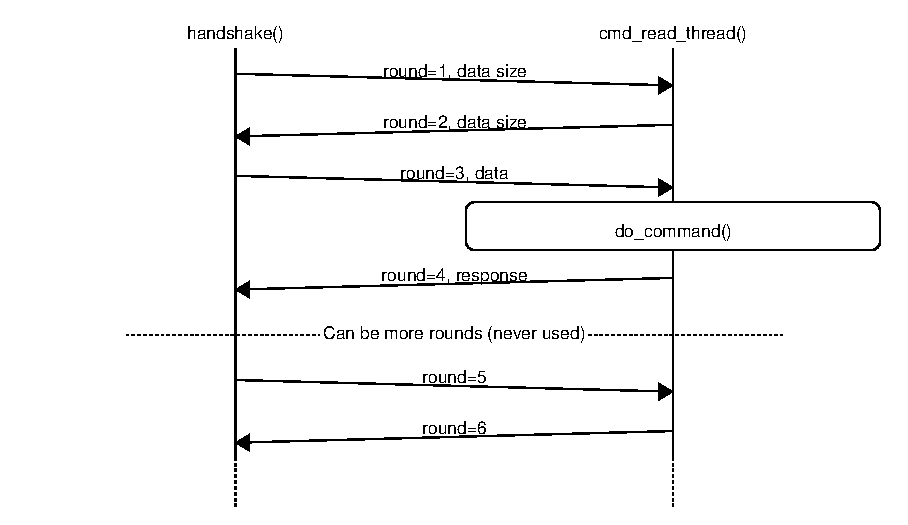
\includegraphics{inline_mscgraph_1}}
\end{DoxyImageNoCaption}
\end{center}
 \} 

Definition at line 200 of file command.\-c.

\hypertarget{command_8c_a94cc0db48e2e582aee04791f7e57581d}{\index{command.\-c@{command.\-c}!path\-\_\-change\-\_\-status@{path\-\_\-change\-\_\-status}}
\index{path\-\_\-change\-\_\-status@{path\-\_\-change\-\_\-status}!command.c@{command.\-c}}
\subsubsection[{path\-\_\-change\-\_\-status}]{\setlength{\rightskip}{0pt plus 5cm}int path\-\_\-change\-\_\-status (
\begin{DoxyParamCaption}
\item[{{\bf connection\-\_\-type} $\ast$}]{conn, }
\item[{int}]{pind, }
\item[{bit\-\_\-8}]{lstatus}
\end{DoxyParamCaption}
)}}\label{command_8c_a94cc0db48e2e582aee04791f7e57581d}
Initiate the change of the path's status


\begin{DoxyParams}{Parameters}
{\em conn} & The connection to use \\
\hline
{\em pind} & Index of path \\
\hline
{\em lstatus} & The new status to use\\
\hline
\end{DoxyParams}
\begin{DoxyReturn}{Returns}
On successful operation returns with 0, otherwise with -\/1. 
\end{DoxyReturn}


Definition at line 292 of file command.\-c.

\hypertarget{command_8c_ab2b8fd2c85bbe180c1b53a5c2318b89b}{\index{command.\-c@{command.\-c}!replicate\-\_\-connection@{replicate\-\_\-connection}}
\index{replicate\-\_\-connection@{replicate\-\_\-connection}!command.c@{command.\-c}}
\subsubsection[{replicate\-\_\-connection}]{\setlength{\rightskip}{0pt plus 5cm}int replicate\-\_\-connection (
\begin{DoxyParamCaption}
\item[{{\bf connection\-\_\-type} $\ast$}]{conn}
\end{DoxyParamCaption}
)}}\label{command_8c_ab2b8fd2c85bbe180c1b53a5c2318b89b}
Send data about a connection to its remote peer


\begin{DoxyParams}{Parameters}
{\em conn} & The connection which should be sent \\
\hline
\end{DoxyParams}
\begin{DoxyReturn}{Returns}
Returns 0 on successful communication 
\end{DoxyReturn}
\begin{DoxyRefDesc}{Todo}
\item[\hyperlink{todo__todo000005}{Todo}]create compact/packed data, don't send the full connection\-\_\-type struct with empty spaces \end{DoxyRefDesc}


\begin{DoxyRefDesc}{Todo}
\item[\hyperlink{todo__todo000006}{Todo}]use port number received from remote \end{DoxyRefDesc}


Definition at line 353 of file command.\-c.


\hypertarget{connection_8c}{\section{/\-Users/kiskele/\-Dropbox/suli/mptcp/source/src/mptlib/connection.c File Reference}
\label{connection_8c}\index{/\-Users/kiskele/\-Dropbox/suli/mptcp/source/src/mptlib/connection.\-c@{/\-Users/kiskele/\-Dropbox/suli/mptcp/source/src/mptlib/connection.\-c}}
}


Basic operations on a connection.  


{\ttfamily \#include \char`\"{}multipath.\-h\char`\"{}}\\*
{\ttfamily \#include \char`\"{}mp\-\_\-local.\-h\char`\"{}}\\*
Include dependency graph for connection.\-c\-:\nopagebreak
\begin{figure}[H]
\begin{center}
\leavevmode
\includegraphics[width=350pt]{connection_8c__incl}
\end{center}
\end{figure}
\subsection*{Functions}
\begin{DoxyCompactItemize}
\item 
void \hyperlink{connection_8c_a5d49f71f053f35e161e9f2f86a026774}{conn\-\_\-start} (\hyperlink{multipath_8h_a8fd58c5c9a4f2463735bc00b930e3b05}{connection\-\_\-type} $\ast$conn)
\item 
void \hyperlink{connection_8c_a887cc9587513ecec784a41aeee070224}{conn\-\_\-stop} (\hyperlink{multipath_8h_a8fd58c5c9a4f2463735bc00b930e3b05}{connection\-\_\-type} $\ast$conn)
\item 
int \hyperlink{connection_8c_ac50355a264286e79337485a750a1e30a}{conn\-\_\-open\-\_\-socket} (\hyperlink{multipath_8h_a8fd58c5c9a4f2463735bc00b930e3b05}{connection\-\_\-type} $\ast$conn)
\item 
\hyperlink{multipath_8h_a8fd58c5c9a4f2463735bc00b930e3b05}{connection\-\_\-type} $\ast$ \hyperlink{connection_8c_a4feb50d1a76600197063cc5936d43c85}{conn\-\_\-search\-\_\-ip} (bit\-\_\-8 version, bit\-\_\-32 $\ast$local, bit\-\_\-32 $\ast$remote, \hyperlink{multipath_8h_a8fd58c5c9a4f2463735bc00b930e3b05}{connection\-\_\-type} $\ast$conn)
\end{DoxyCompactItemize}


\subsection{Detailed Description}
Basic operations on a connection. \begin{DoxyAuthor}{Author}
Almasi, Bela; Debrecen, Hungary 
\end{DoxyAuthor}
\begin{DoxyDate}{Date}
2012.\-08.\-15. 
\end{DoxyDate}
\begin{DoxyCopyright}{Copyright}
Project maintained by Almasi, Bela; Debrecen, Hungary 
\end{DoxyCopyright}


Definition in file \hyperlink{connection_8c_source}{connection.\-c}.



\subsection{Function Documentation}
\hypertarget{connection_8c_ac50355a264286e79337485a750a1e30a}{\index{connection.\-c@{connection.\-c}!conn\-\_\-open\-\_\-socket@{conn\-\_\-open\-\_\-socket}}
\index{conn\-\_\-open\-\_\-socket@{conn\-\_\-open\-\_\-socket}!connection.c@{connection.\-c}}
\subsubsection[{conn\-\_\-open\-\_\-socket}]{\setlength{\rightskip}{0pt plus 5cm}int conn\-\_\-open\-\_\-socket (
\begin{DoxyParamCaption}
\item[{{\bf connection\-\_\-type} $\ast$}]{conn}
\end{DoxyParamCaption}
)}}\label{connection_8c_ac50355a264286e79337485a750a1e30a}
Open the socket of the specified connecton (after 'Load') 
\begin{DoxyParams}{Parameters}
{\em conn} & The connection which needed to be \\
\hline
\end{DoxyParams}


Definition at line 51 of file connection.\-c.

\hypertarget{connection_8c_a4feb50d1a76600197063cc5936d43c85}{\index{connection.\-c@{connection.\-c}!conn\-\_\-search\-\_\-ip@{conn\-\_\-search\-\_\-ip}}
\index{conn\-\_\-search\-\_\-ip@{conn\-\_\-search\-\_\-ip}!connection.c@{connection.\-c}}
\subsubsection[{conn\-\_\-search\-\_\-ip}]{\setlength{\rightskip}{0pt plus 5cm}{\bf connection\-\_\-type}$\ast$ conn\-\_\-search\-\_\-ip (
\begin{DoxyParamCaption}
\item[{bit\-\_\-8}]{version, }
\item[{bit\-\_\-32 $\ast$}]{local, }
\item[{bit\-\_\-32 $\ast$}]{remote, }
\item[{{\bf connection\-\_\-type} $\ast$}]{conn}
\end{DoxyParamCaption}
)}}\label{connection_8c_a4feb50d1a76600197063cc5936d43c85}
Search the connection specified by version, local ip and remote ip keys 
\begin{DoxyParams}{Parameters}
{\em version} & The I\-P Version number (4 or 6) \\
\hline
{\em local} & The local I\-P address \\
\hline
{\em remote} & The remote I\-P address \\
\hline
{\em conn} & The head of the connections list \\
\hline
\end{DoxyParams}
\begin{DoxyReturn}{Returns}
Pointer to the connection or N\-U\-L\-L if not found 
\end{DoxyReturn}


Definition at line 90 of file connection.\-c.

\hypertarget{connection_8c_a5d49f71f053f35e161e9f2f86a026774}{\index{connection.\-c@{connection.\-c}!conn\-\_\-start@{conn\-\_\-start}}
\index{conn\-\_\-start@{conn\-\_\-start}!connection.c@{connection.\-c}}
\subsubsection[{conn\-\_\-start}]{\setlength{\rightskip}{0pt plus 5cm}void conn\-\_\-start (
\begin{DoxyParamCaption}
\item[{{\bf connection\-\_\-type} $\ast$}]{conn}
\end{DoxyParamCaption}
)}}\label{connection_8c_a5d49f71f053f35e161e9f2f86a026774}
Start all connection. Open the connection's socket and start the connection threads 
\begin{DoxyParams}{Parameters}
{\em conn} & The head of the connections list \\
\hline
\end{DoxyParams}


Definition at line 16 of file connection.\-c.

\hypertarget{connection_8c_a887cc9587513ecec784a41aeee070224}{\index{connection.\-c@{connection.\-c}!conn\-\_\-stop@{conn\-\_\-stop}}
\index{conn\-\_\-stop@{conn\-\_\-stop}!connection.c@{connection.\-c}}
\subsubsection[{conn\-\_\-stop}]{\setlength{\rightskip}{0pt plus 5cm}void conn\-\_\-stop (
\begin{DoxyParamCaption}
\item[{{\bf connection\-\_\-type} $\ast$}]{conn}
\end{DoxyParamCaption}
)}}\label{connection_8c_a887cc9587513ecec784a41aeee070224}
Stop all connection. Stop the connection's socket and cancel the connection threads 
\begin{DoxyParams}{Parameters}
{\em conn} & The head of the connections list \\
\hline
\end{DoxyParams}


Definition at line 34 of file connection.\-c.


\hypertarget{inout_8c}{\section{/\-Users/kiskele/\-Dropbox/suli/mptcp/source/src/mptlib/inout.c File Reference}
\label{inout_8c}\index{/\-Users/kiskele/\-Dropbox/suli/mptcp/source/src/mptlib/inout.\-c@{/\-Users/kiskele/\-Dropbox/suli/mptcp/source/src/mptlib/inout.\-c}}
}


Screen and file input/output routines.  


{\ttfamily \#include $<$dirent.\-h$>$}\\*
{\ttfamily \#include $<$sys/types.\-h$>$}\\*
{\ttfamily \#include \char`\"{}multipath.\-h\char`\"{}}\\*
{\ttfamily \#include \char`\"{}mp\-\_\-local.\-h\char`\"{}}\\*
{\ttfamily \#include \char`\"{}auth.\-h\char`\"{}}\\*
Include dependency graph for inout.\-c\-:\nopagebreak
\begin{figure}[H]
\begin{center}
\leavevmode
\includegraphics[width=350pt]{inout_8c__incl}
\end{center}
\end{figure}
\subsection*{Functions}
\begin{DoxyCompactItemize}
\item 
void \hyperlink{inout_8c_aec9920e2075cd9d6b9d3b9fbf2746f93}{tunnel\-\_\-print} (\hyperlink{multipath_8h_ad7a0156e1890c65de09911a138792f6e}{tunnel\-\_\-type} $\ast$\hyperlink{mp__local_8h_a5177b995bc2060be2efb1d21496d1971}{tun})
\item 
void \hyperlink{inout_8c_a1be03958e99ca65e5285a451336b7213}{conn\-\_\-print\-\_\-item} (F\-I\-L\-E $\ast$stream, \hyperlink{multipath_8h_a8fd58c5c9a4f2463735bc00b930e3b05}{connection\-\_\-type} $\ast$conn)
\item 
void \hyperlink{inout_8c_a6a8276ba9c363037221249d3eb8479c0}{conn\-\_\-print} (\hyperlink{multipath_8h_a8fd58c5c9a4f2463735bc00b930e3b05}{connection\-\_\-type} $\ast$conn)
\item 
void \hyperlink{inout_8c_abc49d6855514222bc7dd04f77e1abcac}{conn\-\_\-save} (char $\ast$filename, \hyperlink{multipath_8h_a8fd58c5c9a4f2463735bc00b930e3b05}{connection\-\_\-type} $\ast$\hyperlink{connection_8c_a5d49f71f053f35e161e9f2f86a026774}{conn\-\_\-start})
\item 
void \hyperlink{inout_8c_a74d1430a215c78d2d2516e80ef732303}{conn\-\_\-load\-\_\-dir} (\hyperlink{multipath_8h_a8fd58c5c9a4f2463735bc00b930e3b05}{connection\-\_\-type} $\ast$\hyperlink{connection_8c_a5d49f71f053f35e161e9f2f86a026774}{conn\-\_\-start})
\item 
void \hyperlink{inout_8c_a0bcd14cdbf4cfbc86272401f601c83f8}{conn\-\_\-parser} (F\-I\-L\-E $\ast$fd, \hyperlink{multipath_8h_a8fd58c5c9a4f2463735bc00b930e3b05}{connection\-\_\-type} $\ast$conn)
\item 
\hyperlink{multipath_8h_a8fd58c5c9a4f2463735bc00b930e3b05}{connection\-\_\-type} $\ast$ \hyperlink{inout_8c_ad16eb426ae11cfdd188d4d480b23f563}{conn\-\_\-new} (\hyperlink{multipath_8h_a8fd58c5c9a4f2463735bc00b930e3b05}{connection\-\_\-type} $\ast$conn)
\item 
void \hyperlink{inout_8c_a1a9632e67041bb1907a065022fcd2ec3}{conn\-\_\-load} (char $\ast$filename, \hyperlink{multipath_8h_a8fd58c5c9a4f2463735bc00b930e3b05}{connection\-\_\-type} $\ast$\hyperlink{connection_8c_a5d49f71f053f35e161e9f2f86a026774}{conn\-\_\-start})
\item 
int \hyperlink{inout_8c_acfb42844cff2af7ba8fb07d62cfe5793}{conn\-\_\-diff} (\hyperlink{multipath_8h_a8fd58c5c9a4f2463735bc00b930e3b05}{connection\-\_\-type} $\ast$old, \hyperlink{multipath_8h_a8fd58c5c9a4f2463735bc00b930e3b05}{connection\-\_\-type} $\ast$new)
\item 
int \hyperlink{inout_8c_af53d1429392b1c1dbc9250bf0a6839df}{conn\-\_\-activate} (\hyperlink{multipath_8h_a8fd58c5c9a4f2463735bc00b930e3b05}{connection\-\_\-type} $\ast$conn, int replicate)
\item 
int \hyperlink{inout_8c_a9e0c0df574f096c77d9c8dd3ed816db0}{conn\-\_\-reload} (char $\ast$filename)
\item 
int \hyperlink{inout_8c_af311542df5f335666f4b81cf2e78d8a9}{conn\-\_\-reload\-\_\-dir} ()
\item 
void \hyperlink{inout_8c_a1b2a26c6ac333259fc57aa47c3e7c299}{conn\-\_\-mirror} (\hyperlink{multipath_8h_a8fd58c5c9a4f2463735bc00b930e3b05}{connection\-\_\-type} $\ast$dst, \hyperlink{multipath_8h_a8fd58c5c9a4f2463735bc00b930e3b05}{connection\-\_\-type} $\ast$src)
\item 
void \hyperlink{inout_8c_a6f875afcff66d59c2f2cf2c4587164d8}{calculate\-\_\-weights} (\hyperlink{multipath_8h_a8fd58c5c9a4f2463735bc00b930e3b05}{connection\-\_\-type} $\ast$conn)
\end{DoxyCompactItemize}


\subsection{Detailed Description}
Screen and file input/output routines. \begin{DoxyCopyright}{Copyright}
Project maintained by Almasi, Bela; Debrecen, Hungary 
\end{DoxyCopyright}
\begin{DoxyAuthor}{Author}
Almasi, Bela; Debrecen, Hungary 
\end{DoxyAuthor}
\begin{DoxyDate}{Date}
2012.\-08.\-15.
\end{DoxyDate}
Function calls to manage connections\-: \begin{center}

\begin{DoxyImageNoCaption}
  \mbox{\includegraphics[width=\textwidth,height=\textheight/2,keepaspectratio=true]{dot_inline_dotgraph_1}}
\end{DoxyImageNoCaption}
\end{center}
 

Definition in file \hyperlink{inout_8c_source}{inout.\-c}.



\subsection{Function Documentation}
\hypertarget{inout_8c_a6f875afcff66d59c2f2cf2c4587164d8}{\index{inout.\-c@{inout.\-c}!calculate\-\_\-weights@{calculate\-\_\-weights}}
\index{calculate\-\_\-weights@{calculate\-\_\-weights}!inout.c@{inout.\-c}}
\subsubsection[{calculate\-\_\-weights}]{\setlength{\rightskip}{0pt plus 5cm}void calculate\-\_\-weights (
\begin{DoxyParamCaption}
\item[{{\bf connection\-\_\-type} $\ast$}]{conn}
\end{DoxyParamCaption}
)}}\label{inout_8c_a6f875afcff66d59c2f2cf2c4587164d8}
Calculate packet\-\_\-max values from weight\-\_\-in and weight\-\_\-out parameters. 
\begin{DoxyParams}{Parameters}
{\em conn} & x \\
\hline
\end{DoxyParams}
\begin{DoxyRefDesc}{Todo}
\item[\hyperlink{todo__todo000008}{Todo}]Not implemented \end{DoxyRefDesc}


Definition at line 966 of file inout.\-c.

\hypertarget{inout_8c_af53d1429392b1c1dbc9250bf0a6839df}{\index{inout.\-c@{inout.\-c}!conn\-\_\-activate@{conn\-\_\-activate}}
\index{conn\-\_\-activate@{conn\-\_\-activate}!inout.c@{inout.\-c}}
\subsubsection[{conn\-\_\-activate}]{\setlength{\rightskip}{0pt plus 5cm}int conn\-\_\-activate (
\begin{DoxyParamCaption}
\item[{{\bf connection\-\_\-type} $\ast$}]{conn, }
\item[{int}]{replicate}
\end{DoxyParamCaption}
)}}\label{inout_8c_af53d1429392b1c1dbc9250bf0a6839df}
Setup new or modify existing connection


\begin{DoxyParams}{Parameters}
{\em conn} & The connection needed to add \\
\hline
{\em replicate} & If set to 1, than send this connection to the remote peer \\
\hline
\end{DoxyParams}
\begin{DoxyReturn}{Returns}
Returns 0 if the connection is new or the same as \hyperlink{mp__local_8h_acfb42844cff2af7ba8fb07d62cfe5793}{conn\-\_\-diff()} if the connection is changed 
\end{DoxyReturn}


Definition at line 753 of file inout.\-c.

\hypertarget{inout_8c_acfb42844cff2af7ba8fb07d62cfe5793}{\index{inout.\-c@{inout.\-c}!conn\-\_\-diff@{conn\-\_\-diff}}
\index{conn\-\_\-diff@{conn\-\_\-diff}!inout.c@{inout.\-c}}
\subsubsection[{conn\-\_\-diff}]{\setlength{\rightskip}{0pt plus 5cm}int conn\-\_\-diff (
\begin{DoxyParamCaption}
\item[{{\bf connection\-\_\-type} $\ast$}]{old, }
\item[{{\bf connection\-\_\-type} $\ast$}]{new}
\end{DoxyParamCaption}
)}}\label{inout_8c_acfb42844cff2af7ba8fb07d62cfe5793}
Copy changes from a new temporary connection to the existing 
\begin{DoxyParams}{Parameters}
{\em old} & The existing connection, destination \\
\hline
{\em new} & The new connection, the source \\
\hline
\end{DoxyParams}
\begin{DoxyReturn}{Returns}
Returns with 0, if nothing changed. 
\end{DoxyReturn}


Definition at line 543 of file inout.\-c.

\hypertarget{inout_8c_a1a9632e67041bb1907a065022fcd2ec3}{\index{inout.\-c@{inout.\-c}!conn\-\_\-load@{conn\-\_\-load}}
\index{conn\-\_\-load@{conn\-\_\-load}!inout.c@{inout.\-c}}
\subsubsection[{conn\-\_\-load}]{\setlength{\rightskip}{0pt plus 5cm}void conn\-\_\-load (
\begin{DoxyParamCaption}
\item[{char $\ast$}]{filename, }
\item[{{\bf connection\-\_\-type} $\ast$}]{conn\-\_\-start}
\end{DoxyParamCaption}
)}}\label{inout_8c_a1a9632e67041bb1907a065022fcd2ec3}
Load all connections from a specified file 
\begin{DoxyParams}{Parameters}
{\em filename} & The file to read \\
\hline
{\em conn\-\_\-start} & Can be the last item of the connections list to speed up iteration, but can be the head. If it is N\-U\-L\-L, than \hyperlink{mp__local_8h_ae207e2e02fdde659cbc918346dfc122d}{mp\-\_\-global\-\_\-conn} will be used. \\
\hline
\end{DoxyParams}


Definition at line 494 of file inout.\-c.

\hypertarget{inout_8c_a74d1430a215c78d2d2516e80ef732303}{\index{inout.\-c@{inout.\-c}!conn\-\_\-load\-\_\-dir@{conn\-\_\-load\-\_\-dir}}
\index{conn\-\_\-load\-\_\-dir@{conn\-\_\-load\-\_\-dir}!inout.c@{inout.\-c}}
\subsubsection[{conn\-\_\-load\-\_\-dir}]{\setlength{\rightskip}{0pt plus 5cm}void conn\-\_\-load\-\_\-dir (
\begin{DoxyParamCaption}
\item[{{\bf connection\-\_\-type} $\ast$}]{conn\-\_\-start}
\end{DoxyParamCaption}
)}}\label{inout_8c_a74d1430a215c78d2d2516e80ef732303}
Load all connections from the configuration directory 
\begin{DoxyParams}{Parameters}
{\em conn\-\_\-start} & Can be the last item of the connections list to speed up iteration, but can be the head. If it is N\-U\-L\-L, than \hyperlink{mp__local_8h_ae207e2e02fdde659cbc918346dfc122d}{mp\-\_\-global\-\_\-conn} will be used. \\
\hline
\end{DoxyParams}


Definition at line 270 of file inout.\-c.

\hypertarget{inout_8c_a1b2a26c6ac333259fc57aa47c3e7c299}{\index{inout.\-c@{inout.\-c}!conn\-\_\-mirror@{conn\-\_\-mirror}}
\index{conn\-\_\-mirror@{conn\-\_\-mirror}!inout.c@{inout.\-c}}
\subsubsection[{conn\-\_\-mirror}]{\setlength{\rightskip}{0pt plus 5cm}void conn\-\_\-mirror (
\begin{DoxyParamCaption}
\item[{{\bf connection\-\_\-type} $\ast$}]{dst, }
\item[{{\bf connection\-\_\-type} $\ast$}]{src}
\end{DoxyParamCaption}
)}}\label{inout_8c_a1b2a26c6ac333259fc57aa47c3e7c299}
Create a suitable connection for the local side from the remote configuration


\begin{DoxyParams}{Parameters}
{\em dst} & The destination of the new configuration \\
\hline
{\em src} & The configuration received from the remote host \\
\hline
\end{DoxyParams}
\begin{DoxyRefDesc}{Todo}
\item[\hyperlink{todo__todo000007}{Todo}]search new unused port and send it back to the client \end{DoxyRefDesc}


Definition at line 898 of file inout.\-c.

\hypertarget{inout_8c_ad16eb426ae11cfdd188d4d480b23f563}{\index{inout.\-c@{inout.\-c}!conn\-\_\-new@{conn\-\_\-new}}
\index{conn\-\_\-new@{conn\-\_\-new}!inout.c@{inout.\-c}}
\subsubsection[{conn\-\_\-new}]{\setlength{\rightskip}{0pt plus 5cm}{\bf connection\-\_\-type}$\ast$ conn\-\_\-new (
\begin{DoxyParamCaption}
\item[{{\bf connection\-\_\-type} $\ast$}]{conn}
\end{DoxyParamCaption}
)}}\label{inout_8c_ad16eb426ae11cfdd188d4d480b23f563}
Create a new empty connection and append it to the end of the list 
\begin{DoxyParams}{Parameters}
{\em conn} & Can be the last item of the connections list to speed up iteration, but can be the head. If it is N\-U\-L\-L, than \hyperlink{mp__local_8h_ae207e2e02fdde659cbc918346dfc122d}{mp\-\_\-global\-\_\-conn} will be used. \\
\hline
\end{DoxyParams}
\begin{DoxyReturn}{Returns}
Pointer to the new connection 
\end{DoxyReturn}


Definition at line 469 of file inout.\-c.

\hypertarget{inout_8c_a0bcd14cdbf4cfbc86272401f601c83f8}{\index{inout.\-c@{inout.\-c}!conn\-\_\-parser@{conn\-\_\-parser}}
\index{conn\-\_\-parser@{conn\-\_\-parser}!inout.c@{inout.\-c}}
\subsubsection[{conn\-\_\-parser}]{\setlength{\rightskip}{0pt plus 5cm}void conn\-\_\-parser (
\begin{DoxyParamCaption}
\item[{F\-I\-L\-E $\ast$}]{fd, }
\item[{{\bf connection\-\_\-type} $\ast$}]{conn}
\end{DoxyParamCaption}
)}}\label{inout_8c_a0bcd14cdbf4cfbc86272401f601c83f8}
Read a connection from the configuration file opened and save values in the \hyperlink{structconnection__struct}{connection\-\_\-struct} 
\begin{DoxyParams}{Parameters}
{\em fd} & The file descriptor \\
\hline
{\em conn} & The destination \\
\hline
\end{DoxyParams}


Definition at line 310 of file inout.\-c.

\hypertarget{inout_8c_a6a8276ba9c363037221249d3eb8479c0}{\index{inout.\-c@{inout.\-c}!conn\-\_\-print@{conn\-\_\-print}}
\index{conn\-\_\-print@{conn\-\_\-print}!inout.c@{inout.\-c}}
\subsubsection[{conn\-\_\-print}]{\setlength{\rightskip}{0pt plus 5cm}void conn\-\_\-print (
\begin{DoxyParamCaption}
\item[{{\bf connection\-\_\-type} $\ast$}]{conn}
\end{DoxyParamCaption}
)}}\label{inout_8c_a6a8276ba9c363037221249d3eb8479c0}
Print out all connection's information 
\begin{DoxyParams}{Parameters}
{\em conn} & The head of the connections list \\
\hline
\end{DoxyParams}


Definition at line 140 of file inout.\-c.

\hypertarget{inout_8c_a1be03958e99ca65e5285a451336b7213}{\index{inout.\-c@{inout.\-c}!conn\-\_\-print\-\_\-item@{conn\-\_\-print\-\_\-item}}
\index{conn\-\_\-print\-\_\-item@{conn\-\_\-print\-\_\-item}!inout.c@{inout.\-c}}
\subsubsection[{conn\-\_\-print\-\_\-item}]{\setlength{\rightskip}{0pt plus 5cm}void conn\-\_\-print\-\_\-item (
\begin{DoxyParamCaption}
\item[{F\-I\-L\-E $\ast$}]{stream, }
\item[{{\bf connection\-\_\-type} $\ast$}]{conn}
\end{DoxyParamCaption}
)}}\label{inout_8c_a1be03958e99ca65e5285a451336b7213}
Print out debug information about a connection 
\begin{DoxyParams}{Parameters}
{\em conn} & The connection \\
\hline
\end{DoxyParams}


Definition at line 61 of file inout.\-c.

\hypertarget{inout_8c_a9e0c0df574f096c77d9c8dd3ed816db0}{\index{inout.\-c@{inout.\-c}!conn\-\_\-reload@{conn\-\_\-reload}}
\index{conn\-\_\-reload@{conn\-\_\-reload}!inout.c@{inout.\-c}}
\subsubsection[{conn\-\_\-reload}]{\setlength{\rightskip}{0pt plus 5cm}int conn\-\_\-reload (
\begin{DoxyParamCaption}
\item[{char $\ast$}]{filename}
\end{DoxyParamCaption}
)}}\label{inout_8c_a9e0c0df574f096c77d9c8dd3ed816db0}
Reload all connections' config from a specified file


\begin{DoxyParams}{Parameters}
{\em filename} & The filename which contains the connections \\
\hline
\end{DoxyParams}
\begin{DoxyReturn}{Returns}
The same as \hyperlink{mp__local_8h_acfb42844cff2af7ba8fb07d62cfe5793}{conn\-\_\-diff()} 
\end{DoxyReturn}


Definition at line 825 of file inout.\-c.

\hypertarget{inout_8c_af311542df5f335666f4b81cf2e78d8a9}{\index{inout.\-c@{inout.\-c}!conn\-\_\-reload\-\_\-dir@{conn\-\_\-reload\-\_\-dir}}
\index{conn\-\_\-reload\-\_\-dir@{conn\-\_\-reload\-\_\-dir}!inout.c@{inout.\-c}}
\subsubsection[{conn\-\_\-reload\-\_\-dir}]{\setlength{\rightskip}{0pt plus 5cm}int conn\-\_\-reload\-\_\-dir (
\begin{DoxyParamCaption}
{}
\end{DoxyParamCaption}
)}}\label{inout_8c_af311542df5f335666f4b81cf2e78d8a9}
Reload all connections from the configuration directory \begin{DoxyReturn}{Returns}
The same as \hyperlink{mp__local_8h_acfb42844cff2af7ba8fb07d62cfe5793}{conn\-\_\-diff()} 
\end{DoxyReturn}


Definition at line 861 of file inout.\-c.

\hypertarget{inout_8c_abc49d6855514222bc7dd04f77e1abcac}{\index{inout.\-c@{inout.\-c}!conn\-\_\-save@{conn\-\_\-save}}
\index{conn\-\_\-save@{conn\-\_\-save}!inout.c@{inout.\-c}}
\subsubsection[{conn\-\_\-save}]{\setlength{\rightskip}{0pt plus 5cm}void conn\-\_\-save (
\begin{DoxyParamCaption}
\item[{char $\ast$}]{filename, }
\item[{{\bf connection\-\_\-type} $\ast$}]{conn\-\_\-start}
\end{DoxyParamCaption}
)}}\label{inout_8c_abc49d6855514222bc7dd04f77e1abcac}
Write out the changes of all connection in the specified file


\begin{DoxyParams}{Parameters}
{\em filename} & The file contains the connections \\
\hline
{\em conn\-\_\-start} & The head of the connections list \\
\hline
\end{DoxyParams}


Definition at line 156 of file inout.\-c.

\hypertarget{inout_8c_aec9920e2075cd9d6b9d3b9fbf2746f93}{\index{inout.\-c@{inout.\-c}!tunnel\-\_\-print@{tunnel\-\_\-print}}
\index{tunnel\-\_\-print@{tunnel\-\_\-print}!inout.c@{inout.\-c}}
\subsubsection[{tunnel\-\_\-print}]{\setlength{\rightskip}{0pt plus 5cm}void tunnel\-\_\-print (
\begin{DoxyParamCaption}
\item[{{\bf tunnel\-\_\-type} $\ast$}]{tun}
\end{DoxyParamCaption}
)}}\label{inout_8c_aec9920e2075cd9d6b9d3b9fbf2746f93}
Print out debug informations about the tunnel information 
\begin{DoxyParams}{Parameters}
{\em tun} & The tunnel interface \\
\hline
\end{DoxyParams}


Definition at line 36 of file inout.\-c.


\hypertarget{interface_8c}{\section{/\-Users/kiskele/\-Dropbox/suli/mptcp/source/src/mptlib/interface.c File Reference}
\label{interface_8c}\index{/\-Users/kiskele/\-Dropbox/suli/mptcp/source/src/mptlib/interface.\-c@{/\-Users/kiskele/\-Dropbox/suli/mptcp/source/src/mptlib/interface.\-c}}
}


Basic operations on an interface.  


{\ttfamily \#include \char`\"{}multipath.\-h\char`\"{}}\\*
{\ttfamily \#include \char`\"{}mp\-\_\-local.\-h\char`\"{}}\\*
Include dependency graph for interface.\-c\-:\nopagebreak
\begin{figure}[H]
\begin{center}
\leavevmode
\includegraphics[width=350pt]{interface_8c__incl}
\end{center}
\end{figure}
\subsection*{Functions}
\begin{DoxyCompactItemize}
\item 
void \hyperlink{interface_8c_a9048244ea0041c5239505db3961d2a1b}{mac\-\_\-pton} (char $\ast$src, char $\ast$dst)
\item 
int \hyperlink{interface_8c_a6ae146a6151ff6df02ce01d679d34041}{check\-\_\-loopback} (char $\ast$address)
\item 
void \hyperlink{interface_8c_aff0f41f29b42f2e3b6ea2d479a1ec448}{interface\-\_\-change\-\_\-status} (char $\ast$interface, bit\-\_\-8 status)
\item 
void \hyperlink{interface_8c_a4b11a913e2156ff892f6601f38cf0ae8}{address\-\_\-change\-\_\-status} (bit\-\_\-32 $\ast$addr, bit\-\_\-8 status)
\item 
int \hyperlink{interface_8c_a006b7e907de91c8a393c1716b0308917}{check\-\_\-interface} (char $\ast$interface, int sock)
\item 
void \hyperlink{interface_8c_aaee400b4ef800bf1d289d11cf7737f47}{interface\-\_\-load} (char $\ast$filename, \hyperlink{multipath_8h_ad7a0156e1890c65de09911a138792f6e}{tunnel\-\_\-type} $\ast$\hyperlink{mp__local_8h_a5177b995bc2060be2efb1d21496d1971}{tun}, \hyperlink{multipath_8h_a33e3a32d09de77fbf0e03597b8704196}{interface\-\_\-type} $\ast$interface)
\end{DoxyCompactItemize}


\subsection{Detailed Description}
Basic operations on an interface. \begin{DoxyAuthor}{Author}
Almasi, Bela; Debrecen, Hungary 
\end{DoxyAuthor}
\begin{DoxyDate}{Date}
2012.\-08.\-15. 
\end{DoxyDate}
\begin{DoxyCopyright}{Copyright}
Project maintained by Almasi, Bela; Debrecen, Hungary 
\end{DoxyCopyright}


Definition in file \hyperlink{interface_8c_source}{interface.\-c}.



\subsection{Function Documentation}
\hypertarget{interface_8c_a4b11a913e2156ff892f6601f38cf0ae8}{\index{interface.\-c@{interface.\-c}!address\-\_\-change\-\_\-status@{address\-\_\-change\-\_\-status}}
\index{address\-\_\-change\-\_\-status@{address\-\_\-change\-\_\-status}!interface.c@{interface.\-c}}
\subsubsection[{address\-\_\-change\-\_\-status}]{\setlength{\rightskip}{0pt plus 5cm}void address\-\_\-change\-\_\-status (
\begin{DoxyParamCaption}
\item[{bit\-\_\-32 $\ast$}]{addr, }
\item[{bit\-\_\-8}]{status}
\end{DoxyParamCaption}
)}}\label{interface_8c_a4b11a913e2156ff892f6601f38cf0ae8}
Change the path status for all path of the address 

Definition at line 80 of file interface.\-c.

\hypertarget{interface_8c_a006b7e907de91c8a393c1716b0308917}{\index{interface.\-c@{interface.\-c}!check\-\_\-interface@{check\-\_\-interface}}
\index{check\-\_\-interface@{check\-\_\-interface}!interface.c@{interface.\-c}}
\subsubsection[{check\-\_\-interface}]{\setlength{\rightskip}{0pt plus 5cm}int check\-\_\-interface (
\begin{DoxyParamCaption}
\item[{char $\ast$}]{interface, }
\item[{int}]{sock}
\end{DoxyParamCaption}
)}}\label{interface_8c_a006b7e907de91c8a393c1716b0308917}
Check the status of an interface, value 1 means U\-P 

Definition at line 101 of file interface.\-c.

\hypertarget{interface_8c_a6ae146a6151ff6df02ce01d679d34041}{\index{interface.\-c@{interface.\-c}!check\-\_\-loopback@{check\-\_\-loopback}}
\index{check\-\_\-loopback@{check\-\_\-loopback}!interface.c@{interface.\-c}}
\subsubsection[{check\-\_\-loopback}]{\setlength{\rightskip}{0pt plus 5cm}int check\-\_\-loopback (
\begin{DoxyParamCaption}
\item[{char $\ast$}]{address}
\end{DoxyParamCaption}
)}}\label{interface_8c_a6ae146a6151ff6df02ce01d679d34041}
Check if the address is loopback (Ret. 1=yes) 

Definition at line 47 of file interface.\-c.

\hypertarget{interface_8c_aff0f41f29b42f2e3b6ea2d479a1ec448}{\index{interface.\-c@{interface.\-c}!interface\-\_\-change\-\_\-status@{interface\-\_\-change\-\_\-status}}
\index{interface\-\_\-change\-\_\-status@{interface\-\_\-change\-\_\-status}!interface.c@{interface.\-c}}
\subsubsection[{interface\-\_\-change\-\_\-status}]{\setlength{\rightskip}{0pt plus 5cm}void interface\-\_\-change\-\_\-status (
\begin{DoxyParamCaption}
\item[{char $\ast$}]{interface, }
\item[{bit\-\_\-8}]{status}
\end{DoxyParamCaption}
)}}\label{interface_8c_aff0f41f29b42f2e3b6ea2d479a1ec448}
Change the path status for all path of the intercace 

Definition at line 61 of file interface.\-c.

\hypertarget{interface_8c_aaee400b4ef800bf1d289d11cf7737f47}{\index{interface.\-c@{interface.\-c}!interface\-\_\-load@{interface\-\_\-load}}
\index{interface\-\_\-load@{interface\-\_\-load}!interface.c@{interface.\-c}}
\subsubsection[{interface\-\_\-load}]{\setlength{\rightskip}{0pt plus 5cm}void interface\-\_\-load (
\begin{DoxyParamCaption}
\item[{char $\ast$}]{filename, }
\item[{{\bf tunnel\-\_\-type} $\ast$}]{tun, }
\item[{{\bf interface\-\_\-type} $\ast$}]{interface}
\end{DoxyParamCaption}
)}}\label{interface_8c_aaee400b4ef800bf1d289d11cf7737f47}
Load the data of the interfaces from a file 

Definition at line 116 of file interface.\-c.

\hypertarget{interface_8c_a9048244ea0041c5239505db3961d2a1b}{\index{interface.\-c@{interface.\-c}!mac\-\_\-pton@{mac\-\_\-pton}}
\index{mac\-\_\-pton@{mac\-\_\-pton}!interface.c@{interface.\-c}}
\subsubsection[{mac\-\_\-pton}]{\setlength{\rightskip}{0pt plus 5cm}void mac\-\_\-pton (
\begin{DoxyParamCaption}
\item[{char $\ast$}]{src, }
\item[{char $\ast$}]{dst}
\end{DoxyParamCaption}
)}}\label{interface_8c_a9048244ea0041c5239505db3961d2a1b}
Convert the M\-A\-C address string ('\-:' or '-\/' byte delimiter) to binary form 

Definition at line 15 of file interface.\-c.


\hypertarget{thread_8c}{\section{/\-Users/kiskele/\-Dropbox/suli/mptcp/source/src/mptlib/thread.c File Reference}
\label{thread_8c}\index{/\-Users/kiskele/\-Dropbox/suli/mptcp/source/src/mptlib/thread.\-c@{/\-Users/kiskele/\-Dropbox/suli/mptcp/source/src/mptlib/thread.\-c}}
}


Thread handle functions.  


{\ttfamily \#include $<$sys/time.\-h$>$}\\*
{\ttfamily \#include \char`\"{}multipath.\-h\char`\"{}}\\*
{\ttfamily \#include \char`\"{}mp\-\_\-local.\-h\char`\"{}}\\*
{\ttfamily \#include \char`\"{}cli.\-h\char`\"{}}\\*
{\ttfamily \#include \char`\"{}auth.\-h\char`\"{}}\\*
Include dependency graph for thread.\-c\-:\nopagebreak
\begin{figure}[H]
\begin{center}
\leavevmode
\includegraphics[width=350pt]{thread_8c__incl}
\end{center}
\end{figure}
\subsection*{Functions}
\begin{DoxyCompactItemize}
\item 
void $\ast$ \hyperlink{thread_8c_aeacd27696191f244b5620c704ae1afc3}{tunnel\-\_\-read\-\_\-thread} (void $\ast$arg)
\item 
void $\ast$ \hyperlink{thread_8c_acdb36d82fb3d0ab030bddbb6a987465b}{socket\-\_\-read\-\_\-thread} (void $\ast$arg)
\item 
void $\ast$ \hyperlink{thread_8c_af0542818843fd3fe1827af3a38c79866}{cmd\-\_\-read\-\_\-thread} (void $\ast$arg)
\item 
void $\ast$ \hyperlink{thread_8c_a74eb2b13ac9056bde2d996af471dd7ea}{keepalive\-\_\-send\-\_\-thread} (void $\ast$arg)
\end{DoxyCompactItemize}


\subsection{Detailed Description}
Thread handle functions. \begin{DoxyAuthor}{Author}
Almasi, Bela; Debrecen, Hungary 
\end{DoxyAuthor}
\begin{DoxyDate}{Date}
2012.\-08.\-15. 
\end{DoxyDate}
\begin{DoxyCopyright}{Copyright}
Project maintained by Almasi, Bela; Debrecen, Hungary 
\end{DoxyCopyright}


Definition in file \hyperlink{thread_8c_source}{thread.\-c}.



\subsection{Function Documentation}
\hypertarget{thread_8c_af0542818843fd3fe1827af3a38c79866}{\index{thread.\-c@{thread.\-c}!cmd\-\_\-read\-\_\-thread@{cmd\-\_\-read\-\_\-thread}}
\index{cmd\-\_\-read\-\_\-thread@{cmd\-\_\-read\-\_\-thread}!thread.c@{thread.\-c}}
\subsubsection[{cmd\-\_\-read\-\_\-thread}]{\setlength{\rightskip}{0pt plus 5cm}void$\ast$ cmd\-\_\-read\-\_\-thread (
\begin{DoxyParamCaption}
\item[{void $\ast$}]{arg}
\end{DoxyParamCaption}
)}}\label{thread_8c_af0542818843fd3fe1827af3a38c79866}
The thread to read commands from the cmd socket 

Definition at line 115 of file thread.\-c.

\hypertarget{thread_8c_a74eb2b13ac9056bde2d996af471dd7ea}{\index{thread.\-c@{thread.\-c}!keepalive\-\_\-send\-\_\-thread@{keepalive\-\_\-send\-\_\-thread}}
\index{keepalive\-\_\-send\-\_\-thread@{keepalive\-\_\-send\-\_\-thread}!thread.c@{thread.\-c}}
\subsubsection[{keepalive\-\_\-send\-\_\-thread}]{\setlength{\rightskip}{0pt plus 5cm}void$\ast$ keepalive\-\_\-send\-\_\-thread (
\begin{DoxyParamCaption}
\item[{void $\ast$}]{arg}
\end{DoxyParamCaption}
)}}\label{thread_8c_a74eb2b13ac9056bde2d996af471dd7ea}
The thread to send keepalive messages 

Definition at line 258 of file thread.\-c.

\hypertarget{thread_8c_acdb36d82fb3d0ab030bddbb6a987465b}{\index{thread.\-c@{thread.\-c}!socket\-\_\-read\-\_\-thread@{socket\-\_\-read\-\_\-thread}}
\index{socket\-\_\-read\-\_\-thread@{socket\-\_\-read\-\_\-thread}!thread.c@{thread.\-c}}
\subsubsection[{socket\-\_\-read\-\_\-thread}]{\setlength{\rightskip}{0pt plus 5cm}void$\ast$ socket\-\_\-read\-\_\-thread (
\begin{DoxyParamCaption}
\item[{void $\ast$}]{arg}
\end{DoxyParamCaption}
)}}\label{thread_8c_acdb36d82fb3d0ab030bddbb6a987465b}
The thread to read data from the connection's socket 

Definition at line 87 of file thread.\-c.

\hypertarget{thread_8c_aeacd27696191f244b5620c704ae1afc3}{\index{thread.\-c@{thread.\-c}!tunnel\-\_\-read\-\_\-thread@{tunnel\-\_\-read\-\_\-thread}}
\index{tunnel\-\_\-read\-\_\-thread@{tunnel\-\_\-read\-\_\-thread}!thread.c@{thread.\-c}}
\subsubsection[{tunnel\-\_\-read\-\_\-thread}]{\setlength{\rightskip}{0pt plus 5cm}void$\ast$ tunnel\-\_\-read\-\_\-thread (
\begin{DoxyParamCaption}
\item[{void $\ast$}]{arg}
\end{DoxyParamCaption}
)}}\label{thread_8c_aeacd27696191f244b5620c704ae1afc3}
The thread to read data from the tunnel interface 

Definition at line 19 of file thread.\-c.


\hypertarget{trim_8c}{\section{/\-Users/kiskele/\-Dropbox/suli/mptcp/source/src/mptlib/trim.c File Reference}
\label{trim_8c}\index{/\-Users/kiskele/\-Dropbox/suli/mptcp/source/src/mptlib/trim.\-c@{/\-Users/kiskele/\-Dropbox/suli/mptcp/source/src/mptlib/trim.\-c}}
}


Public domain implementations of in-\/place string trim functions.  


{\ttfamily \#include $<$ctype.\-h$>$}\\*
{\ttfamily \#include $<$string.\-h$>$}\\*
Include dependency graph for trim.\-c\-:\nopagebreak
\begin{figure}[H]
\begin{center}
\leavevmode
\includegraphics[width=202pt]{trim_8c__incl}
\end{center}
\end{figure}
\subsection*{Functions}
\begin{DoxyCompactItemize}
\item 
char $\ast$ \hyperlink{trim_8c_a897834a6ab83257290ce165e99366d43}{ltrim} (char $\ast$s)
\item 
char $\ast$ \hyperlink{trim_8c_acdfc0f8ee81107535c88f945cbfeb305}{rtrim} (char $\ast$s)
\item 
char $\ast$ \hyperlink{trim_8c_a8bd9dd70049fb4e00071d0d73bb8d2a0}{trim} (char $\ast$s)
\item 
char $\ast$ \hyperlink{trim_8c_a5274950e8822c442ca0993a7f50f13d9}{basename} (char $\ast$string)
\end{DoxyCompactItemize}


\subsection{Detailed Description}
Public domain implementations of in-\/place string trim functions. \begin{DoxyAuthor}{Author}
Michael Burr \href{mailto:michael.burr@nth-element.com}{\tt michael.\-burr@nth-\/element.\-com} 
\end{DoxyAuthor}
\begin{DoxyDate}{Date}
2010 
\end{DoxyDate}


Definition in file \hyperlink{trim_8c_source}{trim.\-c}.



\subsection{Function Documentation}
\hypertarget{trim_8c_a5274950e8822c442ca0993a7f50f13d9}{\index{trim.\-c@{trim.\-c}!basename@{basename}}
\index{basename@{basename}!trim.c@{trim.\-c}}
\subsubsection[{basename}]{\setlength{\rightskip}{0pt plus 5cm}char$\ast$ basename (
\begin{DoxyParamCaption}
\item[{char $\ast$}]{string}
\end{DoxyParamCaption}
)}}\label{trim_8c_a5274950e8822c442ca0993a7f50f13d9}
Strip down path and get filename \begin{DoxyAuthor}{Author}
Kelemen Tamas 
\end{DoxyAuthor}


Definition at line 64 of file trim.\-c.

\hypertarget{trim_8c_a897834a6ab83257290ce165e99366d43}{\index{trim.\-c@{trim.\-c}!ltrim@{ltrim}}
\index{ltrim@{ltrim}!trim.c@{trim.\-c}}
\subsubsection[{ltrim}]{\setlength{\rightskip}{0pt plus 5cm}char$\ast$ ltrim (
\begin{DoxyParamCaption}
\item[{char $\ast$}]{s}
\end{DoxyParamCaption}
)}}\label{trim_8c_a897834a6ab83257290ce165e99366d43}
Strip whitespace from the beginning of a string 

Definition at line 15 of file trim.\-c.

\hypertarget{trim_8c_acdfc0f8ee81107535c88f945cbfeb305}{\index{trim.\-c@{trim.\-c}!rtrim@{rtrim}}
\index{rtrim@{rtrim}!trim.c@{trim.\-c}}
\subsubsection[{rtrim}]{\setlength{\rightskip}{0pt plus 5cm}char$\ast$ rtrim (
\begin{DoxyParamCaption}
\item[{char $\ast$}]{s}
\end{DoxyParamCaption}
)}}\label{trim_8c_acdfc0f8ee81107535c88f945cbfeb305}
Strip whitespace from the end of a string 

Definition at line 32 of file trim.\-c.

\hypertarget{trim_8c_a8bd9dd70049fb4e00071d0d73bb8d2a0}{\index{trim.\-c@{trim.\-c}!trim@{trim}}
\index{trim@{trim}!trim.c@{trim.\-c}}
\subsubsection[{trim}]{\setlength{\rightskip}{0pt plus 5cm}char$\ast$ trim (
\begin{DoxyParamCaption}
\item[{char $\ast$}]{s}
\end{DoxyParamCaption}
)}}\label{trim_8c_a8bd9dd70049fb4e00071d0d73bb8d2a0}
Strip whitespace from the beginning and end of a string 

Definition at line 54 of file trim.\-c.


\hypertarget{tunnel_8c}{\section{/\-Users/kiskele/\-Dropbox/suli/mptcp/source/src/mptlib/tunnel.c File Reference}
\label{tunnel_8c}\index{/\-Users/kiskele/\-Dropbox/suli/mptcp/source/src/mptlib/tunnel.\-c@{/\-Users/kiskele/\-Dropbox/suli/mptcp/source/src/mptlib/tunnel.\-c}}
}


Tunnel handling functions.  


{\ttfamily \#include \char`\"{}multipath.\-h\char`\"{}}\\*
{\ttfamily \#include \char`\"{}mp\-\_\-local.\-h\char`\"{}}\\*
Include dependency graph for tunnel.\-c\-:\nopagebreak
\begin{figure}[H]
\begin{center}
\leavevmode
\includegraphics[width=350pt]{tunnel_8c__incl}
\end{center}
\end{figure}
\subsection*{Macros}
\begin{DoxyCompactItemize}
\item 
\hypertarget{tunnel_8c_ab3de656908348a477ef4b2109ec0289d}{\#define {\bfseries O\-T\-U\-N\-S\-E\-T\-I\-F\-F}~(('T'$<$$<$ 8) $|$ 202)}\label{tunnel_8c_ab3de656908348a477ef4b2109ec0289d}

\end{DoxyCompactItemize}
\subsection*{Functions}
\begin{DoxyCompactItemize}
\item 
int \hyperlink{tunnel_8c_a054a3e1dd3bd936c3e4cd5c5e9876fe0}{tunnel\-\_\-start} (\hyperlink{multipath_8h_ad7a0156e1890c65de09911a138792f6e}{tunnel\-\_\-type} $\ast$\hyperlink{mp__local_8h_a5177b995bc2060be2efb1d21496d1971}{tun})
\item 
int \hyperlink{tunnel_8c_aa5f3a4c2c65b76f72d1e203ead2f593e}{cmd\-\_\-open\-\_\-socket} (\hyperlink{multipath_8h_ad7a0156e1890c65de09911a138792f6e}{tunnel\-\_\-type} $\ast$\hyperlink{mp__local_8h_a5177b995bc2060be2efb1d21496d1971}{tun})
\item 
int \hyperlink{tunnel_8c_aaf277918c024742ecabe2f367c750fd1}{tunnel\-\_\-stop} (\hyperlink{multipath_8h_ad7a0156e1890c65de09911a138792f6e}{tunnel\-\_\-type} $\ast$\hyperlink{mp__local_8h_a5177b995bc2060be2efb1d21496d1971}{tun})
\end{DoxyCompactItemize}


\subsection{Detailed Description}
Tunnel handling functions. \begin{DoxyAuthor}{Author}
Almasi, Bela; Debrecen, Hungary 
\end{DoxyAuthor}
\begin{DoxyDate}{Date}
2012.\-08.\-15. 
\end{DoxyDate}
\begin{DoxyCopyright}{Copyright}
Project maintained by Almasi, Bela; Debrecen, Hungary 
\end{DoxyCopyright}


Definition in file \hyperlink{tunnel_8c_source}{tunnel.\-c}.



\subsection{Function Documentation}
\hypertarget{tunnel_8c_aa5f3a4c2c65b76f72d1e203ead2f593e}{\index{tunnel.\-c@{tunnel.\-c}!cmd\-\_\-open\-\_\-socket@{cmd\-\_\-open\-\_\-socket}}
\index{cmd\-\_\-open\-\_\-socket@{cmd\-\_\-open\-\_\-socket}!tunnel.c@{tunnel.\-c}}
\subsubsection[{cmd\-\_\-open\-\_\-socket}]{\setlength{\rightskip}{0pt plus 5cm}int cmd\-\_\-open\-\_\-socket (
\begin{DoxyParamCaption}
\item[{{\bf tunnel\-\_\-type} $\ast$}]{tun}
\end{DoxyParamCaption}
)}}\label{tunnel_8c_aa5f3a4c2c65b76f72d1e203ead2f593e}
Open and bind the cmd socket 

Definition at line 79 of file tunnel.\-c.

\hypertarget{tunnel_8c_a054a3e1dd3bd936c3e4cd5c5e9876fe0}{\index{tunnel.\-c@{tunnel.\-c}!tunnel\-\_\-start@{tunnel\-\_\-start}}
\index{tunnel\-\_\-start@{tunnel\-\_\-start}!tunnel.c@{tunnel.\-c}}
\subsubsection[{tunnel\-\_\-start}]{\setlength{\rightskip}{0pt plus 5cm}int tunnel\-\_\-start (
\begin{DoxyParamCaption}
\item[{{\bf tunnel\-\_\-type} $\ast$}]{tun}
\end{DoxyParamCaption}
)}}\label{tunnel_8c_a054a3e1dd3bd936c3e4cd5c5e9876fe0}
Open and config the tunnel interface 

Definition at line 18 of file tunnel.\-c.

\hypertarget{tunnel_8c_aaf277918c024742ecabe2f367c750fd1}{\index{tunnel.\-c@{tunnel.\-c}!tunnel\-\_\-stop@{tunnel\-\_\-stop}}
\index{tunnel\-\_\-stop@{tunnel\-\_\-stop}!tunnel.c@{tunnel.\-c}}
\subsubsection[{tunnel\-\_\-stop}]{\setlength{\rightskip}{0pt plus 5cm}int tunnel\-\_\-stop (
\begin{DoxyParamCaption}
\item[{{\bf tunnel\-\_\-type} $\ast$}]{tun}
\end{DoxyParamCaption}
)}}\label{tunnel_8c_aaf277918c024742ecabe2f367c750fd1}
Stop and close the tunnel device 

Definition at line 131 of file tunnel.\-c.


\hypertarget{main_8c}{\section{/\-Users/kiskele/\-Dropbox/suli/mptcp/source/src/mptsrv/main.c File Reference}
\label{main_8c}\index{/\-Users/kiskele/\-Dropbox/suli/mptcp/source/src/mptsrv/main.\-c@{/\-Users/kiskele/\-Dropbox/suli/mptcp/source/src/mptsrv/main.\-c}}
}


Main code of the server application.  


{\ttfamily \#include $<$string.\-h$>$}\\*
{\ttfamily \#include \char`\"{}multipath.\-h\char`\"{}}\\*
{\ttfamily \#include \char`\"{}mp\-\_\-local.\-h\char`\"{}}\\*
Include dependency graph for main.\-c\-:\nopagebreak
\begin{figure}[H]
\begin{center}
\leavevmode
\includegraphics[width=350pt]{main_8c__incl}
\end{center}
\end{figure}
\subsection*{Functions}
\begin{DoxyCompactItemize}
\item 
int \hyperlink{main_8c_ae66f6b31b5ad750f1fe042a706a4e3d4}{main} ()
\end{DoxyCompactItemize}


\subsection{Detailed Description}
Main code of the server application. 

Definition in file \hyperlink{main_8c_source}{main.\-c}.



\subsection{Function Documentation}
\hypertarget{main_8c_ae66f6b31b5ad750f1fe042a706a4e3d4}{\index{main.\-c@{main.\-c}!main@{main}}
\index{main@{main}!main.c@{main.\-c}}
\subsubsection[{main}]{\setlength{\rightskip}{0pt plus 5cm}int main (
\begin{DoxyParamCaption}
{}
\end{DoxyParamCaption}
)}}\label{main_8c_ae66f6b31b5ad750f1fe042a706a4e3d4}
Main function of server applcation that creates the tunnel interface, starts threads and configures the connections 

Definition at line 18 of file main.\-c.


%--- End generated contents ---

% Index
\newpage
\phantomsection
\addcontentsline{toc}{part}{Index}
\printindex

\end{document}
